\def\fileversion{v1.0} \def\filedate{2018/07/20}
%% Package and Class "uiucthesis2009" for use with LaTeX2e.
\documentclass[edeposit,fullpage,11pt]{uiucthesis2009}
\usepackage[acronym,toc]{glossaries}
\usepackage{graphicx}
\usepackage{pdflscape}
%\newacronym{<++>}{<++>}{<++>}
%\newacronym{<++>}{<++>}{<++>}

\newacronym{MTHM}{MTHM}{metric ton of heavy metal}
\newacronym{XS}{XS}{cross-sections}
\newacronym{AO}{AO}{Axial Offset}
\newacronym{PCI}{PCI}{Pellet-Cladding Interaction}
\newacronym{PCMI}{PCMI}{Pellet-Cladding Material Interaction}
\newacronym{lhr}{LHR}{Linear Hear Rate}
\newacronym{SCC}{SCC}{Stress Corrosion Cracking}
\newacronym{MPS}{MPS}{Missing Pellet Surface}

\newacronym{BOC}{BOC}{Beginning of Cycle}
\newacronym{BOL}{BOL}{Beginning of Life}
\newacronym{HZP}{HZP}{Hot Zero Power}
\newacronym{HFP}{HFP}{Hot Full Power}
\newacronym{CASL}{CASL}{Consortium for Advanced Simulation of Light Water Reactors}
\newacronym{IFBA}{IFBA}{Integral Fuel Burnable Absorber}
\newacronym{UMich}{UMich}{University of Michigan}
\newacronym{NCSU}{NCSU}{North Carolina State University}
\newacronym{ORNL}{ORNL}{Oak Ridge National Laboratory}
\newacronym{CMFD}{CMFD}{Coarse Mesh Finite Diference}
\newacronym{INL}{INL}{Idaho National Laboratory}
\newacronym{MOOSE}{MOOSE}{Multiphysics Object Oriented Simulation Environment }
\newacronym{ITC}{ITC}{Isothermal Temperature Coefficient }
\newacronym{CRW}{CRW}{Control Rod Worth}




\newacronym{DOE}{DOE}{Department of Energy}
\newacronym{EPA}{EPA}{Environmental Protection Agency}
\newacronym{EFPD}{EFPD}{Effective Full Power Days}
\newacronym{EOC}{EOC}{End of Cycle}
\newacronym{GWDMT}{GWDMT}{GigaWatt Day per Metric Ton}
\newacronym{DRWM}{DRWM}{Dynamic Rod Worth Measurement}


\newacronym{LWR}{LWR}{Light Water Reactor}
\newacronym{LPPT}{LPPT}{Low Power Physics Tests}

\newacronym{MIT}{MIT}{the Massachusetts Institute of Technology}


\newacronym{NEUP}{NEUP}{Nuclear Energy University Programs}
\newacronym{NPRE}{NPRE}{Department of Nuclear, Plasma, and Radiological Engineering}
\newacronym{NRC}{NRC}{Nuclear Regulatory Commission}

\newacronym{PARCS}{PARCS}{Purdue Advanced Reactor Core Simulator}
\newacronym{PATHS}{PATHS}{PARCS Advanced Thermal Hydraulic Solver}
\newacronym{PWR}{PWR}{Pressurized Water Reactor}
\newacronym{BWR}{BWR}{Boiling Water Reactor}

\newacronym{UOX}{UOX}{uranium oxide}
\newacronym{UQ}{UQ}{uncertainty quantification}
\newacronym{US}{U.S.}{United States}
\newacronym{UIUC}{UIUC}{University of Illinois at Urbana-Champaign}
\newacronym{VV}{V\&V}{verification and validation}
\newacronym{VERA}{VERA}{Virtual Enviromnment for Reactor Analysis}
\newacronym{VERACS}{VERA-CS}{VERA Core Simulator}
\newacronym{BEAVRS}{BEAVRS}{Benchmark for Evaluation And Validation of Reactor Simulations}
\newacronym{BW}{B\&W-1484}{Babcock and Wilcox critical experiments Series 1484}



\begin{document}

\title{Investigation of Pellet Clad Interaction during Load-Follow\\
       Operation in a Pressurized Water Reactor using VERA-CS}
\author{Daniel John O'Grady}
\department{Nuclear, Plasma, and Radiological Engineering}
\schools{B.S., University of Illinois at Urbana-Champaign, 2017}
\msthesis
\advisor{Tomasz Kozlowski}
\degreeyear{2018}
\committee{Professor Tomasz Kozlowski, Advisor}%\\Professor Katherine Huff}
\maketitle

\frontmatter

%% Create an abstract that can also be used for the ProQuest abstract.
%% Note that ProQuest truncates their abstracts at 350 words.
\begin{abstract}
This is a comprehensive study on the effect load-follow operation has on fuel failure risk in a PWR. 
PWR1, a commercial reactor that performed load-follow power maneuvers in cycle 21, was modeled using VERA-CS starting in cycle 17. 
The effects of a jump-in approach were shown to be negligible after two cycles of standard depletion.
Both low power physics tests and critical boron comparisons show excellent agreement between the VERA-CS predictions and the plant measured data after cycle 19.
In addition to cycle depletion, five load-follow power maneuvers in the first 24 days of cycle 21 were simulated using hourly depletion steps. 
VERA-CS predictions of this time period showed an overestimation of the axial offset behavior during the load-follow operation but the overall reactivity of the core showed good agreement.

The linear heat rate and coolant temperature calculated by VERA-CS were used as boundary conditions for BISON fuel performance calculations.
Using the maximum hoop stress as the indicator of fuel failure risk, the different load-follow power maneuvers were compared to the initial start-up ramp.
The maximum clad hoop stress occurred during the start-up ramp and was estimated to be 94 MPa, the subsequent maneuvers showed similar magnitudes regardless of the change in power. 
No correlation was observed between the characteristics of the load-follow power maneuver and the resulting maximum clad hoop stress. 
Neither the depth of the decrease in power, hold period, nor intermediate power steps showed a variation in the maximum clad hoop stress observed after a return to full power ramp this early in the cycle.

To reduce the number of fuel performance calculations required to determine the safety of a power maneuver, a pin based screening process based on a weighted change in conditioned power was developed.
By selecting the top 1000 fuel rods showing a positive weighted change in linear heat rate, the limiting fuel pin for the maneuver is contained, with most of the additional selected pins showing elevated hoop stresses. 
%Early cycle results show an undesired dependence on position resulting in low risk fuel pins being selected during the screening process.
\end{abstract}

%% Create a dedication in italics with no heading, centered vertically
%% on the page.
%\begin{dedication}
%To Father and Mother.
%\end{dedication}

%% Create an Acknowledgements page, many departments require you to
%% include funding support in this.
\chapter*{Acknowledgments}

This project would not have been possible without the support of many people. 
Many thanks to my adviser, Tomasz Kozlowski and group members, Majdi, Chen, Katarzyna, Guojun, Travis, and Dean who read my numerous revisions and listened to all of the obstacles that arose during this project.
Also many thanks to the ORNL and UM staff members, Andrew Godfrey, Shane Stimpson, Kevin Clarno, Mark Baird, Scott Palmtag, Brendan Kochunas, Daniel Jaybay and Thomas Downar, who offered guidance and support.
Invaluable support was also received from the BISON team, including Richard Williamson and Russel Gardner.
And finally, thanks to my girlfriend, parents, and numerous friends who endured this long process with me, always offering support and distractions.

This research was supported in part under an Integrated University Program Graduate Fellowship and an appointment to the Oak Ridge National Laboratory HERE Program, sponsored by the U.S. Department of Energy and administered by the Oak Ridge Institute for Science and Education
The work made use of the resources of the High Performance Computing Center at Idaho National Laboratory, which is supported by the Office of Nuclear Energy of the U.S. Department of Energy and the Nuclear Science User Facilities under Contract No. DE­AC07­05ID14517.

%% The thesis format requires the Table of Contents to come
%% before any other major sections, all of these sections after
%% the Table of Contents must be listed therein (i.e., use \chapter,
%% not \chapter*).  Common sections to have between the Table of
%% Contents and the main text are:
%%
%% List of Tables
%% List of Figures
%% List Symbols and/or Abbreviations
%% etc.

\tableofcontents
\listoftables
\listoffigures

%% Create a List of Abbreviations. The left column
%% is 1 inch wide and left-justified
\chapter{List of Abbreviations}

\begin{symbollist*}
\item[PWR]     Pressurized Water Reactor
\item[BWR]     Boiling Water Reactor
\item[AO]      Axial Offset
\item[BOC]     Beginning of Cycle
\item[EOC]     End of Cycle
\item[BOL]     Beginning of Life
\item[EOL]     End of Life
\item[GWDMT]   GigaWatt Day per Metric Ton
\item[HZP]     Hot Zero Power
\item[HFP]     Hot Full Power
\item[LPPT]    Low Power Physics Tests
\item[ITC]     Isothermal Temperature Coefficient 
\item[CRW]     Control Rod Worth
\item[LHR]     Linear Hear Rate
\item[PIE]     Post Irradiation Examination
\item[PCI]     Pellet-Cladding Interaction
\item[PCMI]    Pellet-Cladding Material Interaction
\item[SCC]     Stress Corrosion Cracking
\item[MPS]     Missing Pellet Surface
\item[CDI]     Cumulative Damage Index
\item[CASL]    Consortium for Advanced Simulation of Light Water Reactors
\item[VERA]    Virtual Environment for Reactor Analysis
\item[VERA-CS] VERA Core Simulator
\end{symbollist*}

%% Create a List of Symbols. The left column
%% is 0.7 inch wide and centered
%\chapter{List of Symbols}

%\begin{symbollist}[0.7in]
%\item[$\tau$] Time taken to drink one cup of coffee.
%\item[$\mu$g] Micrograms (of caffeine, generally).
%\end{symbollist}

\mainmatter

%%%%%%%%%%%%%%%%%%%%%%%%%%%%%%%%%%%%%%%%%%%%%%%%%%%%%%%%%
%%%%%%%%%%%%%%%%%%%%%%%%%%%%%%%%%%%%%%%%%%%%%%%%%%%%%%%%%
\chapter{Introduction}
%%%%%%%%%%%%%%%%%%%%%%%%%%%%%%%%%%%%%%%%%%%%%%%%%%%%%%%%%
%%%%%%%%%%%%%%%%%%%%%%%%%%%%%%%%%%%%%%%%%%%%%%%%%%%%%%%%%

In the \gls{US}, nuclear power generation has high fixed costs and low variable costs. 
As a result, utilities have traditionally sought to operate nuclear stations at full power from \gls{BOC} to \gls{EOC}. 
More recently, the deregulation of the energy market and the emergence of intermittent renewable energy sources have caused load-follow operation to become a more attractive option for nuclear generation. 

The deregulation of the energy market has forced utilities to compete against each other to sell electricity regionally.
The beneficiary of this competition are the customers, who are guaranteed fair prices for electricity and will not be footing the bill for an inefficient/uneconomical utility project. %need citation
Nuclear stations have typically been able to economically compete within deregulated markets because the typical plant lifetime of at least 20 years allows owners to spread out the fixed costs.
Recently, the low price of natural gas and government subsidized renewable energy sources, such as wind and solar, have made nuclear stations appear less profitable.   

%%%%%%%%%%%%%%%%%%%%%%%%%%%%%%%%%%%%%%%%%%%%%%%%%%%%%%%%%
\section{Background and Motivation}
%%%%%%%%%%%%%%%%%%%%%%%%%%%%%%%%%%%%%%%%%%%%%%%%%%%%%%%%%

In 2016, the \gls{US} had approximately 7\% of its total electricity generation coming from wind and solar power \cite{u.s_energy_information_administration_electricity_2016}. 
This share is likely to increase as the \gls{US} continues to move away from fossil fuels and towards a ``greener" energy future.
As a result of this increase, in combination with the deregulation of the energy market, the price of electricity has become volatile. 
At certain times, the price of selling electricity within a region can even become negative due to a sudden increase in renewable energy output and a low market demand \cite{paraschiv_impact_2014}. 
In some areas, negative electricity prices are further increased due to the fact that large generating facilities would rather sell at a loss than decrease their power level. 
This preference is caused by the high capital cost and relatively low variable costs of large generating facilities \cite{lokhov_load-following_2011}.

Nuclear stations are typically one of these large generating facilities.
As a result of the large construction costs and the fixed number of required on-site staff members, most utilities prefer to keep a reactor at full power, as it is easiest to maintain constant power. 
If a nuclear station operated in load-follow mode instead of remaining at full power, the efficient of the plant would likely increase.
This is because during load-follow operation, a nuclear station will vary its power output in response to the anticipated demand to better suit the market needs, stabilizing the price of electricity.
Theoretically, the currently operating U.S. plants were all designed with the maneuverability to respond to such change in demand \cite{lokhov_technical_2011}.
In fact, many of the reactors in France already participate in load-following maneuvers with the help of grey control rods \cite{lokhov_technical_2011}.
Grey control rods are similar to standard \gls{PWR} control rods but have significantly less rod worth \cite{yousefpour_improvement_2000}.
The low rod worth allows them to be used for reactivity control without putting significant stress on the surrounding fuel. 
In the \gls{US}, grey rods are not present in \gls{PWR}, which introduces additional stresses on the fuel cladding, increasing the complexity of load-follow operation \cite{lokhov_technical_2011}.
  
Previous load follow demonstrations have been performed on \gls{US} \gls{PWR}s.
In the 1970's Indian Point underwent a series of load-follow power maneuvers, where 50 \% power swings were performed using ramp rates that varied between 0.25 and 5.0 \% power/minute \cite{sipush_load-follow_1976}.
The primary purpose of this study was to demonstrate the plant's ability to maintain control over the \gls{AO} during/following the power maneuvers. 
If control over the \gls{AO} is lost, control rods may not have the strength to effect the core power distribution in the presence of local xenon concentrations \cite{sipush_load-follow_1976}.
With insufficient control over the flux profile, local linear heat rates could exceed safety margins.

In order to mitigate this possibility, \gls{PWR} primarily use the critical boron concentration to modify the power level while making minor control rod insertion and inlet temperature modifications to manage the core \gls{AO} \cite{meyer_improved_1978}.  
Even though safety margins are maintained, the insertion of control rods and the response of the local xenon concentrations can lead to significant changes in local pin powers throughout the core.
Due to thermal expansion changes in local power can cause fuel to swell or contract \cite{gartner_power_1984}. 
If a utility chooses to ramp down the reactor during times of excess high supply the fuel pellets can contract.
When the decision is made to return the reactor back to full power, the rate at which the power can be increased is limited by the thermal expansion of the fuel pellets \cite{gartner_power_1984}.
A sudden expansion of the fuel pellet has the potential to exert additional stress on the cladding, commonly referred to as \gls{PCMI}.
\gls{PCMI} can lead to fuel failure, fission product release, by \gls{PCI} and has been extensively investigated since the early 1970s.

\subsection{Pellet Clad Interaction}

\gls{PCI} induced fuel failure is the result of \gls{PCMI} and environmental contributions.
\gls{PCMI} is best described as the material interaction at the pellet-clad interface which creates a stress state on the fuel cladding \cite{kennard_pci_2016}.
This stress state is normally quantified using the maximum cladding hoop stress, which occurs at the inner radius of the cladding.
In a cylindrical fuel rod, hoop stress, shown in Figure \ref{fig:hoop_stress_cite}, is a function of the pressure being exerted on the cladding through fuel pellet contact as well as the pressure difference between the gap and coolant.

\begin{figure}
\begin{center}
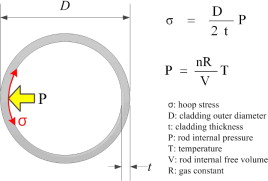
\includegraphics[width=0.5\linewidth]{./Figures/hoop_stress_cite.jpg}
\caption{Visualization of the hoop stress acting on the fuel cladding using the thin wall approximation \cite{kook_review_2013}}
\label{fig:hoop_stress_cite}
\end{center}
\end{figure}

To determine the magnitude of the cladding hoop stress the shape of the fuel pellets mush be accurately known.
The shape of the fuel pellets controls the volume of plenum, influencing the gap pressure, and in the case that the gap has closed, the fuel pellet's shape is restrained by the cladding. 
Many different factors contribute to the shape of the fuel pellet including temperature of the fuel, fission product inventory, power history and manufacturing characteristics.
During power maneuvers, the fuel temperature is the most significant as it determines the degree to which the fuel expands.
To further complicate the geometry of the fuel pellet, nonuniform thermal expansion during the initial ramp to power causes radial cracks to form within a pellet \cite{capps_evaluation_2016}.
These cracks, in addition to thermal expansion, lead to shear forces and hoop stress on the inner radius of the fuel cladding.
  
In addition to the mechanical stress being exerted on the cladding, environmental contributions, chemical or geometrical in nature, have an adverse effect on the claddings integrity.
Chemical environments arise from the release of fission products from the fuel pellet.
Iodine and cadmium-in-cesium are considered to be the most corrosive fission products released from the pellet \cite{capps_evaluation_2016}. 
In the presence of prolonged \gls{PCMI}, the corrosive chemical environment causes inter granular crack propagation, or \gls{SCC}, through the zircaloy-based cladding.
This type of cladding failure is commonly referred to as \gls{PCI}--\gls{SCC}, or ``classical \gls{PCI}."

Geometric contributions to \gls{PCI} are a result of irregularities in the fuel pellet shape.
Typical \gls{LWR} fuel pellets are a ceramic $UO_2$ cylinder with a height of approximately 1 cm and dishes and chamfers on the top and bottom of the pellet.
Hundreds of these pellets are stacked into a single fuel rod, with approximately 60,000 fuel rods in a \gls{LWR} core.
The shear quantity of fuel pellets ordered by a utility makes it impossible for a fuel vendor to ensure no pellet has a defect.
The most common defect is a \gls{MPS} where part of the fuel pellet has chipped off during manufacturing.
This chip causes asymmetric expansion of the pellet during power maneuvers leading to an increased local stress on the fuel cladding \cite{capps_evaluation_2016}. 
If the induced stress exceeds the yield stress of the cladding, brittle failure is likely to occur.
This type of cladding failure is commonly referred to as \gls{PCI}-\gls{MPS}, as the missing surface is the critical feature in causing the failure.


%%%%%%%%%%%%%%%%%%%%%%%%%%%%%%%%%%%%%%%%%%%%%%%%%%%%%%%%%
\section{Literature Review}
%%%%%%%%%%%%%%%%%%%%%%%%%%%%%%%%%%%%%%%%%%%%%%%%%%%%%%%%%

In the early 1970's a string of fuel failures in \gls{BWR} led to the first classification of \gls{PCI} induced fuel failure.  
Shortly after, \gls{PCI} induced fuel failures were found in \gls{PWR} and determined to be an inherent problem in \gls{LWR} zircaloy based fuels. %Find citation
The majority of these failures were observed during or shortly after power maneuvers from hot zero power.
To reduce the risk of failure, fuel manufactures made design modifications and began to provide power ramping guidelines \cite{kennard_pci_2016}.
These ramp guideline were particularly conservative and focused primarily on \gls{BOC} power ramps. 
Since then, \gls{PCI} has been extensively studied in order to increase the efficiency of reactor start-up and minimize the number of fuel failures.
%In order to extend the results of these studies to load follow operation, the driving forces of \gls{PCI} must be analyzed to determine their significance mid cycle power ramps.
 
%%%%%%
%First Paper
%%%%%%
Cox \cite{cox_pellet-clad_1990} performed an extensive review of the work done on zircaloy fuel failures caused by \gls{PCI} up to 1972.
It was found that fuel pellet geometry is the most significant factor in \gls{PCI}.
The strain on the cladding is determined by
\begin{enumerate}
\item manufactured gap size
\item shape of the fuel pellet
\item effect of the chamfers and groves.
\end{enumerate} 
In addition to manufacturing defects, ceramic $UO_2$ fuel pellets also experience a number of geometric changes as a function of iradiation and temperature/power level.
These changes include, but are not limited to, fuel pellet  densification, cracking, relocation, and thermal expansion. 
Pellet cracking and relocation contribute significantly to the strain experienced by the cladding due to the differential movement of the pellets relative to one another.
This differential movement is further intensified  by the locking of crack edges into cracks within the cladding and the local coefficient of friction between the pellet/cladding.
At high exposure the coefficient of friction can approach infinity as fission products have escaped the fuel pellet and cemented the pellet to the cladding, leading to intensified stresses during power maneuvers. 

In addition to the contribution the fuel pellet geometry has on the local strain, the cladding material and geometry can determine how the cladding will respond to such strain.
Both the wall thickness to diameter ratio and creep rate of the cladding effect the magnitude of the initial stress and the rate at which the stress decays.
The total stress imposed on the cladding is a function of the maximum power, which determines the total expansion of the fuel pellet, and also the change in power during a power ramp, which determines the increment in cladding strain.
Cox goes on to highlight the importance of a corrosive agent at causing \gls{PCI}, noting that Iodine and Cadmium-in-Cesium are the largest contributors to the corrosive environment at the cladding surface.
To minimize the risk of \gls{PCI}, Cox emphasized the importance of fuel conditioning and holds at intermediate power during large power ramps.

The term fuel conditioning is commonly used by researchers and industry representatives when discussing power maneuvers, yet the quantitative definition of conditioning can be difficult to find.
Capps et al. described fuel condition as the state of the fuel rod when considering the changes in the fuel, cladding and gap \cite{capps_evaluation_2016}.
Many of these changes are a result of the pellet and cladding's response to radiation and heat transfer, for example
\begin{itemize}
\item fuel pellet cracking and relocation are caused by the thermal expansion of $UO_2$,
\item fuel pellet densification is caused by radiation exposure,
\item fuel pellet swelling is caused by fission product accumulation,
\item grain growth in fuel pellets is caused by elevated temperatures,
\item and creep deformation in the pellet and the cladding occur due to elevated temperatures and radiation exposure.
\end{itemize}
Due to the fact that all of these changes are dependent on the local power and exposure, a concrete definition of fuel conditioning is difficult to create.
Rather, fuel conditioning describes the ability of the fuel rod to respond to rapid changes in power \cite{capps_evaluation_2016}.
During conditioning the cladding is able to relieve some of the stress experienced during a power increases.
The chemical environment at the surface of the pellet is also influenced during the conditioning period \cite{cox_pellet-clad_1990}.
Together these effects reduce the propagation of cracks, limiting the possibility of \gls{PCI} induced fuel failure.
%%%%%%

%%%%%%
%Second Paper
%%%%%%
Jernkvist \cite{jernkvist_model_1995} developed a model for predicting \gls{PCI} induced fuel failure based on crack initiation and growth.
Jernkvist's model stressed three key parameters involved in \gls{PCI},
\begin{itemize} 
\item cladding stress and strain are extremely localized, 
\item fuel rod failure due to \gls{PCI} is normally a result of a sudden power increase 
\item \gls{PCI} induced failure within a reactor core shows strong variability.
\end{itemize}
Due to the presence of internal flaws within the cladding, Jernkvist neglected the intergranular process and only considered transgranular crack growth.
In order to account for the stochastic nature of \gls{PCI} in reactor cores, a probabilistic treatment of the initial crack size was used.
The crack propagation velocity was then determined by the stress, temperature, and iodine concentration at the tip of the crack.
Using a finite element solver, Jernkvist calculated the stress at the tip of the crack.
If the stress was greater than the iodine stress corrosion crack threshold, the velocity was determined using a correlation requiring the temperature and iodine concentration.
To simplify the determination of the iodine concentration, a correlation was used based on the power and fuel burnup.
It was then assumed that all of the iodine collects at the pellet-pellet interface and radial pellet cracks.

With the velocity of the crack propagation known, the time to cladding failure can be calculated.
Using an artificial power history, Jernkvist provides an example where the coefficient of friction is varied for the pellet-clad interface.
At sufficiently high coefficients of friction, the local stress on the cladding is high enough to grow the crack through the cladding, i.e. cause fuel failure.
Jernkvist's study shows the importance of accurately determining the stress within the cladding when trying to predict cladding failure.
Additionally, it highlights the need for a coupled multiphysics approach as the coefficient of friction at the pellet-clad interface is a function of temperature and burnup.
%%%%%%

%%%%%%
%Third Paper
%%%%%%
One of the computational codes that attempts to incorporate this multiphysics approach is FALCON \cite{montgomery_falcon_1997}.
FALCON is a fully coupled, thermo-mechanical, two dimensional finite element computer code being developed by ANATECH.
Building on the material properties provided in MATPRO, FALCON has the ability to simulate $UO_2$ pellet relocation, fission gas release and zircaloy cladding thermal creep.

FALCON has been extensively benchmarked and is commonly used by contractors and utilities to mitigate the risk of \gls{PCI} induced fuel failure.
Lyon et al. \cite{lyon_pci_2009} used FALCON  to determine a criteria for mitigating \gls{PCI} induced fuel failure during power ramps.
The authors point out that power ramp rate restrictions, which are normally set by fuel vendors, and fuel conditioning are not reliable at mitigating the risk of \gls{PCI}. 
Instead, these practices lead to restrictive constraints on plant operation.

Another criteria that is commonly suggested by fuel vendors is the implementation of a stress-based threshold.
Unfortunately, stress based thresholds are normally unable to distinguish between failed and non failed fuel rods, leading to a conservative threshold when applied to power maneuvers \cite{lyon_pci_2009}.
 Lyon et al. proposes a mechanistic approach that incorporates \gls{PCMI} and \gls{SCC} based cumulative damage.

Similar to Jernkavist,  Lyon et al. recognized that cladding failure due to \gls{SCC} occurs in two stages, crack incubation and crack propagation.
The \gls{CDI} model in FALCON accounts for both of these stages using a cumulative damage process, where damage accumulation is linear with time.
This allows the damage fraction, $D$, to be defined as 
\begin{equation}\label{eqn:paper_3_eqn_1}
D = \int \frac{dt}{\bar{t}}
\end{equation}
where $\bar{t}$ is the time-to-failure.
The time-to-failure of a material is normally measured in an \gls{SCC} out-of-pile test and is defined as
\begin{equation}
\bar{t} = f(\sigma,\sigma_y,\sigma_{ref},B,T)
\end{equation}
where $\sigma$ is the applied hoop stress, $\sigma_y$ is the materials yield strength, $\sigma_{ref}$ is a burnup dependent function, $B$ is the burnup of the fuel, and $T$ is the temperature.
It is important to note that Equation \ref{eqn:paper_3_eqn_1} only applies to a single power maneuver, therefore $D$ must be summed over all power maneuvers. 
Experience has shown that $D$ exhibits logarithmic behavior with stress, therefore it should be interpreted probabilistically, where $D=1$ represents a 50\% failure probability while $D=0.1$ and $D=10$ imply  $<5$\% and $>59$\% failure probability, respectively.
In order to account for the possibility that cladding stress can drop below the \gls{SCC} threshold during ramps and environmental difference can arise between in-pile and out-of-pile fuel rods, an adjustable single valued parameter $\beta$ is introduced to the \gls{CDI} model. 
\begin{equation}
D = \sum \frac{\delta t_i}{\beta \bar{t_i}}
\end{equation}

In order to demonstrate the accuracy of a \gls{CDI} based criteria, Lyon et al. simulated 14 fuel rods from the Studsvik Over Ramp, Super Ramp and Trans Ramp IV program as well as rods from a CEA/OSIRIS ramp program using FALCON \cite{killeen_experimental_2004}. 
These simulations were broken into three parts, first a steady state two dimensional, R-Z, depletion simulation is performed using the power histories of each rod.
The results of these simulations are then used as the initial conditions for transient R-Z simulations of the different power ramps under investigation.
Finally, an R-$\theta$ model containing discrete fuel cracks is created for the axial location which experienced the highest R-Z hoop stress.
This simulation provides the fuel pins maximum clad hoop stress and \gls{CDI} which can then be used to determine a failure threshold criteria.

After validating the steady state simulations against \gls{PIE} measurements, Lyon et al. performed the transient analysis for all of the fuel rods. 
The power history of fuel rod Q11/1, along with the maximum cladding hoop stress and \gls{CDI} are shown in Figure \ref{fig:paper_3_res}.
It is observed that the \gls{CDI} only changes during sharp power ramps while the hoop stress more closely follows the power profile.

Using the results of all 14 fuel rods, the authors established a statistical failure criteria using both hoop stress and \gls{CDI}.
A 550 MPa maximum clad hoop stress  and a \gls{CDI} of 5.85 were determined to signify a 50\% chance of rod failure.
Using the 50\% chance as a hard cut off between non-failed and failed rods, the authors evaluated how each of the criteria performed using the 14 fuel rods.
The peak stress was able to correctly predict the behavior of eight out of the 14 fuel rods while the \gls{CDI} predicted the behavior of 13 out of the 14 rods.
Although this work does show the superiority of a \gls{CDI} based criteria, the training set and validation set are the same set, in addition the set is considerably small.
Additionally, the power ramps used during the test program are extreme and are unlikely to be performed during standard operation or load-follow operation.
As a result, further validation is needed before deciding if a \gls{CDI} based criteria is reliable.
 
\begin{figure}
\begin{tabular}{cc}
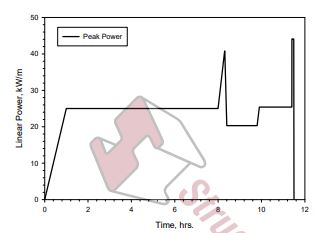
\includegraphics[width=0.5\linewidth]{./Figures/lyon_image_6.JPG} & 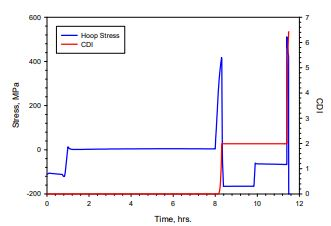
\includegraphics[width=0.5\linewidth]{./Figures/lyon_image_7.JPG}
\end{tabular}
\caption{The Power history (left), Falcon predicted hoop stress and Falcon predicted CDI (right) for Q11/1 of the Studsvik ramp program \cite{lyon_pci_2009}}
\label{fig:paper_3_res}
\end{figure}
%%%%%%


%%%%%%
%Fourth Paper
%%%%%%
Similar to Lyon et al., Capps et al. \cite{capps_pci_2017} used BISON to investigate fuel rods that failed during the start up ramp of a commercial \gls{PWR}.
Before Capps et al. could begin applying failure thresholds to fuel rods under investigation, the thresholds needed to be determined using BISON as the thresholds are specific to the performance code.
To do so, the Studsvik ramp tests were implemented in BISON using a four step process \cite{killeen_experimental_2004}.
The first three steps follow the same methodology used by Lyon et al, R-Z depletion followed by an R-Z fuel performance calculation, ending with a R-$\theta$ fuel performance calculation at the axial location with the highest hoop stress.
The fourth step, which is unique to BISON, is a three dimensional R-$\theta$-Z fuel performance simulation of the entire rod. %check to make sure entire rod was simlated
Although BISON is capable of computing \gls{CDI}, the authors only report the failure thresholds based on the peak cladding hoop stress.
The results of both the R-$\theta$ and the three dimensional simulations were consistent with the results presented by Lyon et al.
The authors observed that the hoop stress calculated in the three dimensional study was consistently higher than the hoop stress from the R-$\theta$ study.
This signifies the importance the pellet's height has on the cladding stress.
Although the three dimensional stress was elevated, no clear cutoff was observed to distinguish the failed fuel rods from the intact fuel rods.
For this reason, a statistical approach was developed for both the R-$\theta$ and the three dimensional simulations.

Using the same four step methodology, the authors performed fuel performance simulations on several fuel rods from the commercial \gls{PWR}.
Two different cycle startup ramps were investigated; the first cycle contained three failed fuel rods and the second contained a single failed fuel rod.
The power histories for the R-Z depletion were provided by Westinghouse and are assumed to be from a nodal core simulator.
Before analyzing any of the BISON results, the authors observed important characteristics from the fuel rods' power histories.
Two of the failed rods in the first cycle were exposed to aggressive linear heat rates during their initial cycle.
This led to the rods accumulating high burnups and the closing of the pellet-clad gap.
The third failed rod saw a significant increase in its linear heat rate after its initial cycle.
As noted in the previous works, these characteristics are strong indicators of each rod's conditioning.

In order to account for the change in cladding material, zirc4 in the Studsvik tests, zirlo in the commercial reactor, Capps et al. scaled the 5\% failure thresholds to 395 MPa for the R-$\theta$ and 446 MPa for the three dimensional predictions.
The peak cladding hoop stress for all three of the failed rods was predicted to be below the threshold in both simulations.
Additionally, two of the non-failed rods that were predicted to have peak cladding hoop stress above the threshold. 
This led the authors to conclude that ``classical" \gls{PCI} could not be the cause of the failure.
After introducing a \gls{MPS} to each of the simulated rods, all peak cladding hoop stresses fell above the 5\% failure threshold.
Furthermore, one of the fuel rods was confirmed to have a \gls{MPS} during a \gls{PIE}, confirming the predictions of the simulation.

In order to reduce the probability of \gls{PCI} induced failure, classic or \gls{MPS} induced, Exelon implemented strict power ramp rates and began to introduce power holds during return to full power ramps \cite{capps_pci_2017}.
Capps et al. investigated the effects of these restrictions on the cladding hoop stress and found that they could reduce the peak stress by approximately 50 MPa.
Even though this led to a decrease in risk, fuel failure was still experienced during an initial power maneuver.
This suggests that pellet defects are a major contributor to fuel failure during power maneuvers. 
Using the restrictive power history developed by Exelon, Capps et al. performed a sensitivity study on the maximum clad hoop stress as a function of \gls{MPS} width.

Fuel specifications limit the dimension of a \gls{MPS} to 60 mils, but widths up to 125 mils have been observed during \gls{PIE} \cite{aleshin_effect_2010}.
For this reason, \gls{MPS} with lengths ranging from 60 to 140 mils were simulated using 2D and 3D BISON simulations. 
The hoop stress resulting from a \gls{MPS} is a result of pellet thermal expansion. 
As the pellet expands the missing face does not exert an outward force on the cladding, causing the cladding to bend at the edges of the \gls{MPS}.
In 2D simulations the hoop stress increases linearly with the length of the \gls{MPS}, with a width of 110 mils increasing the probability of failure to 50\%.
These simulations are inherently flawed as adiabatic boundary conditions are applied to the top and bottom the fuel slice, resulting in the limitation that heat must be conducted radially.
As the missing pellet surface grows, the heat transfer across the gap degrades leading to an increase in pellet temperature.
This increase in temperature causes the pellet to continue to swell, exerting additional pressure on the cladding.

In reality, the heat will flow in the direction of the least resistance, i.e. axial conduction will compensate for the reduction in heat transfer across the gap.
This effect is captured in the 3D simulations, which show miniscule changes in the maximum fuel temperature as a function of \gls{MPS} width.
A \gls{MPS} width of 100 mils was found to result in a 50\% chance of fuel failure during the restrictive power ramps.
Unfortunately, the 3D simulations were performed using an infinite coefficient of friction between the pellet and cladding, causing elevated stresses in the cladding when compared to the 2D simulations.
This prevents a meaningful comparison on the effect fuel temperature has on the failure thresholds in 2D and 3D simulations.
%%%%%%

%%%%%%
%Fifth Paper
%%%%%%

In order to more comprehensively understand the effect pellet defects have on the cladding, Capps et al. studied the individual effects of fuel cracks and \gls{MPS} \cite{capps_evaluation_2016}.
The stress on the cladding caused by pellet cracks is a function of the crack length and the spacing in between cracks.
As the crack spacing increases within the fuel pellet the number of cracks within the pellet decreases.
This causes the opening of a single pellet to increase, which increases the tangential stress on the cladding at the cracks opening.
It is typically found that commercial fuel has six to ten radial cracks, which helps to reduce the stress on the cladding \cite{oguma_cracking_1983}. 

The length of a fuel pellet crack characterizes the compliance of the fuel pellet to its manufactured cylindrical shape.
As the crack length increases, the fuel pellet is less compliant and creates a shear stress on the cladding.
Capps et al. found that the shear stress exerted begins to saturate when the crack length approaches 50\% of the pellet radius.
Although the stress on the cladding has saturated, the stress at the tip of the crack is larger than the fracture strength.
This suggests that the crack will continue to propagate until it has reached approximately 70\% of the pellet radius.

In most cases, \gls{MPS} are accompanied by cracks.
This makes it necessary to incorporate pellet cracks when determining the effect of \gls{MPS}.
Unlike pellet cracks, \gls{MPS} causes hoop stresses within the clad through bending forces.
This hoop stress shows a saturation as the \gls{MPS} width increases.
In addition to the width of the \gls{MPS}, the shape of the defect has a strong effect on the maximum hoop stress.
It is typical to simulate \gls{MPS} as flat defects, although it is more likely they will be concave in shape. 
This concavity further reduces the pellet-gap conductivity causing a rise in the fuel temperature and an increase in the maximum hoop stress.

Although 2D simulations are useful in determining the effect of fuel cracks and \gls{MPS}, they are inherently flawed as many of the axial effects are lost in the boundary conditions.
In addition to the loss of heat transfer in the axial direction, structural support is not taken into consideration as the \gls{MPS} has an infinite height.
Unfortunately, three dimensional contact makes the simulation of cracks and \gls{MPS} difficult, and prohibits a full length fuel rod from being simulated in three dimensions. 
To work around this, Capps et al. simulated a stack of five discrete fuel pellets with a \gls{MPS} included in the center fuel pellet.
The results of the three dimensional study showed that axial contributions reduce the maximum cladding hoop stress by 7 to 15 \%.
Although this reduction is significant, the trends observed in the two dimensional studies did not change.
Therefore, fuel performance studies can be conducted in two dimensions as long as the thresholds for stress were determined using consistent two dimensional studies.
%%%%%%

%%%%%%
%Sixth Paper
%%%%%%
Knowing the statistical thresholds and the importance of cladding defects in regards to fuel failure, analysts can determine the risk of fuel failure for a given core power maneuver.
Typically the initial ramp to full power is given the most attention but in the case of load-load follow operation all power maneuvers will need to be analyzed to determine the risk of fuel failure.
Unfortunately, it is far too computationally expensive to perform a \gls{PCI} focused fuel performance simulation for all of the rods within the core for each of the ramps under consideration.
In order to reduce the number of simulations required most utilities or contractors will focus on a small number of assemblies within the core.
Kennard et al. describes how to go about reducing the 193 fuel assemblies found in a commercial \gls{PWR} down to about 6 limiting assemblies \cite{kennard_pci_2016}.
The screening process  looks to see if 1) an assembly has seen a significant power increase since its previous cycle, 2) exposure falls above a critical value, and 3) the ratio of the maximum power to the conditioned power is large.
Typically a core simulator will provide the predicted pin powers, which are needed to screen the power maneuver.
The assemblies selected are then considered the limiting assemblies for the power maneuver and are analyzed using a fuel performance simulator.
%Mention how this load-follow makes it difficult to implement this screening
Kennard et al. applied this screening process to a commercial \gls{PWR} start up ramp.
The pins within the limiting fuel assemblies were analyzed using FALCON and the methodology presented by Lyon et al. \cite{lyon_pci_2009}.

Based on the 1\% failure threshold for a FALCON fuel performance simulation, Kennard et al. made recommendations to mitigate the risk of \gls{PCI} induced fuel failures for a number of generic operating conditions.
Two recommendations are made in regards to load-follow operation, the first being the importance of maintaining \gls{AO} control.
During a return to full power maneuver, the local xenon concentrations and moderator temperature coefficient will cause the core \gls{AO} to swing.
If the \gls{AO} swing is significant, enough local power levels may exceed conditioned power levels causing a sudden expansion of the fuel pellets.
Strong control over the \gls{AO} will reduce this risk, mitigating the chance of fuel failure.
The second recommendation is better described as a warning.
Kennard et al. warn that local power uncertainties can increase the stress experienced during returns to full power after a reduced power hold.
This recommendation highlights the importance of accurately knowing local power at the pin cell level.
Many core simulators would use a nodal core simulator and pin power reconstruction to calculate the pin power as a function of time.
This reconstruction is likely to introduce uncertainty in the pin powers leading to an increased uncertainty in the fuel performance results.

In this work, \gls{VERACS} is used to simulate load-follow operation of a commercial \gls{PWR}.
\gls{VERACS} is capable of accurately predicting pin powers allowing for reduced uncertainty in fuel performance results.
In addition to the reduced uncertainty in fuel performance results, the fideleity of the \gls{VERACS} results allow for a pin focused screening process in place of an assembly based process.
By focusing on individual pins the number of necessary fuel performance calculations can be reduced allowing for the examination of more severe load-follow maneuvers.
In the remaining chapters the results of load-follow focused fuel performance calculations will be presented for the operating history of a commercial \gls{PWR}.
In Chapter two the preliminary work required to perform fuel performance calculations will be presented, including a description of the PWR1 model and the \gls{VERACS} code. 
A detailed description of the BISON fuel performance code and the pin based screening process are presented in Chapter 3.
In Chapter 4 the results of the fuel performance calculation will be analyzed using the pin based screening process.
In closing, the conclusions drawn from this work and possible future extensions will be presented in Chapter 5.


%%%%%%
%%%%%%%%%%%%%%%%%%%%%%%%%%%%%%%%%%%%%%%%%%%%%%%%%%%%%%%%%
%%%%%%%%%%%%%%%%%%%%%%%%%%%%%%%%%%%%%%%%%%%%%%%%%%%%%%%%%
\chapter{PWR1}
%%%%%%%%%%%%%%%%%%%%%%%%%%%%%%%%%%%%%%%%%%%%%%%%%%%%%%%%%
%%%%%%%%%%%%%%%%%%%%%%%%%%%%%%%%%%%%%%%%%%%%%%%%%%%%%%%%%
The \gls{UIUC} partnered with the \gls{CASL} to investigate load-follow operations in a PWR. 
The objective of the work was to investigate the effects of load-follow operation specific to an operating PWR. 
At request of the owner, the reactor chosen was not to be disclosed but it will be referred to as PWR1.
PWR1 was chosen due to the significant load-follow maneuvers that occurred during operating cycle 21. 
To provide an accurate power history and isotopic composition for the load-follow operation during cycle 21, it was decided that a jump-in depletion would be performed starting four cycles earlier, i.e. cycle 17. 
This decision is due to core loading patterns that include assemblies shuffled from two cycles prior (e.g. cycle 21 includes assemblies introduced in cycle 19, whereas cycle 19 includes assemblies introduced in cycle 17). 
By the advice of \gls{CASL}, it was determined that any approximations of power histories or isotopic compositions introduced to the model in cycle 17 would have a negligible effect on the results obtained in cycle 21.


\section{PWR 1 Model Description}
PWR1 is a four-loop Westinghouse PWR.
Each core loading has 193 Westinghouse 17x17 fuel assemblies, comprised of 264 fuel rods, 24 guide tubes and one instrumentation tube. 
Each fuel rod consists of two axial regions, a blanket and a mid-section. 
Within the mid-section, the enrichment of each rod is selected to ensure sufficiently low power peaking and a desired cycle length. 
The enrichment within the blanket is typically lower than the mid-section to reduce axial leakage from the core. 
In addition, a thin layer of zirconium diboride may be applied to the mid-section of a fuel pin. 
This thin coating, known as an \gls{IFBA}, allows for greater reactivity control throughout the life of the fuel rod. 
One drawback of IFBA coating is an increase in the plenum pressure as the absorber is burned. 
To compensate for this increase in pressure, annular pellets are used within the blanket region. 

The VERA model includes the core plates, nozzles, gaps, two Inconel and six Zircaloy spacer grids, and three intermediate flow mixer (IFM) grids. 
In addition, a total of twenty-four different assembly designs were used in the various cycles of interest. 
All core and assembly geometry details necessary to model PWR1 in VERA-CS were collected and provided by the industry partner.


\subsection{VERA-CS}
\gls{CASL}'s primary computational tool suite, VERA-CS, incorporates coupled physics and science-based models, state-of-the-art numerical methods and modern computational science applied to reactor core simulation. 
VERA-CS achieves this task by integrating three well-developed physics simulators with other supporting sub-components. 
In the present work, we used the deterministic neutronics solver, MPACT, coupled with the sub-channel thermal-hydraulics solver, CTF, to perform detailed simulations down to single-pin resolution, as shown in Figure \ref{fig:workflow}.
The fuel performance (thermo-mechanical) code, BISON, was used to construct fuel temperature tables, which related the temperature of the fuel to the temperature of the cladding as a function of burnup and linear heat rate.  
A significant advantage of the VERA-CS system is the reduction of overall modeling effort by unifying all solver components into a single user-friendly input specification (called VERAin) and a single binary output file.
The VERAin input file is an ASCII text input based on geometric and material descriptions that is parsed out to each code (physics) component through built-in tools. 
Below is a brief description of two of the primary simulators that are part of the VERA-CS system used for this work, the BISON fuel performance simulator will be presented in Chapter 3.

\begin{figure}
\begin{center}
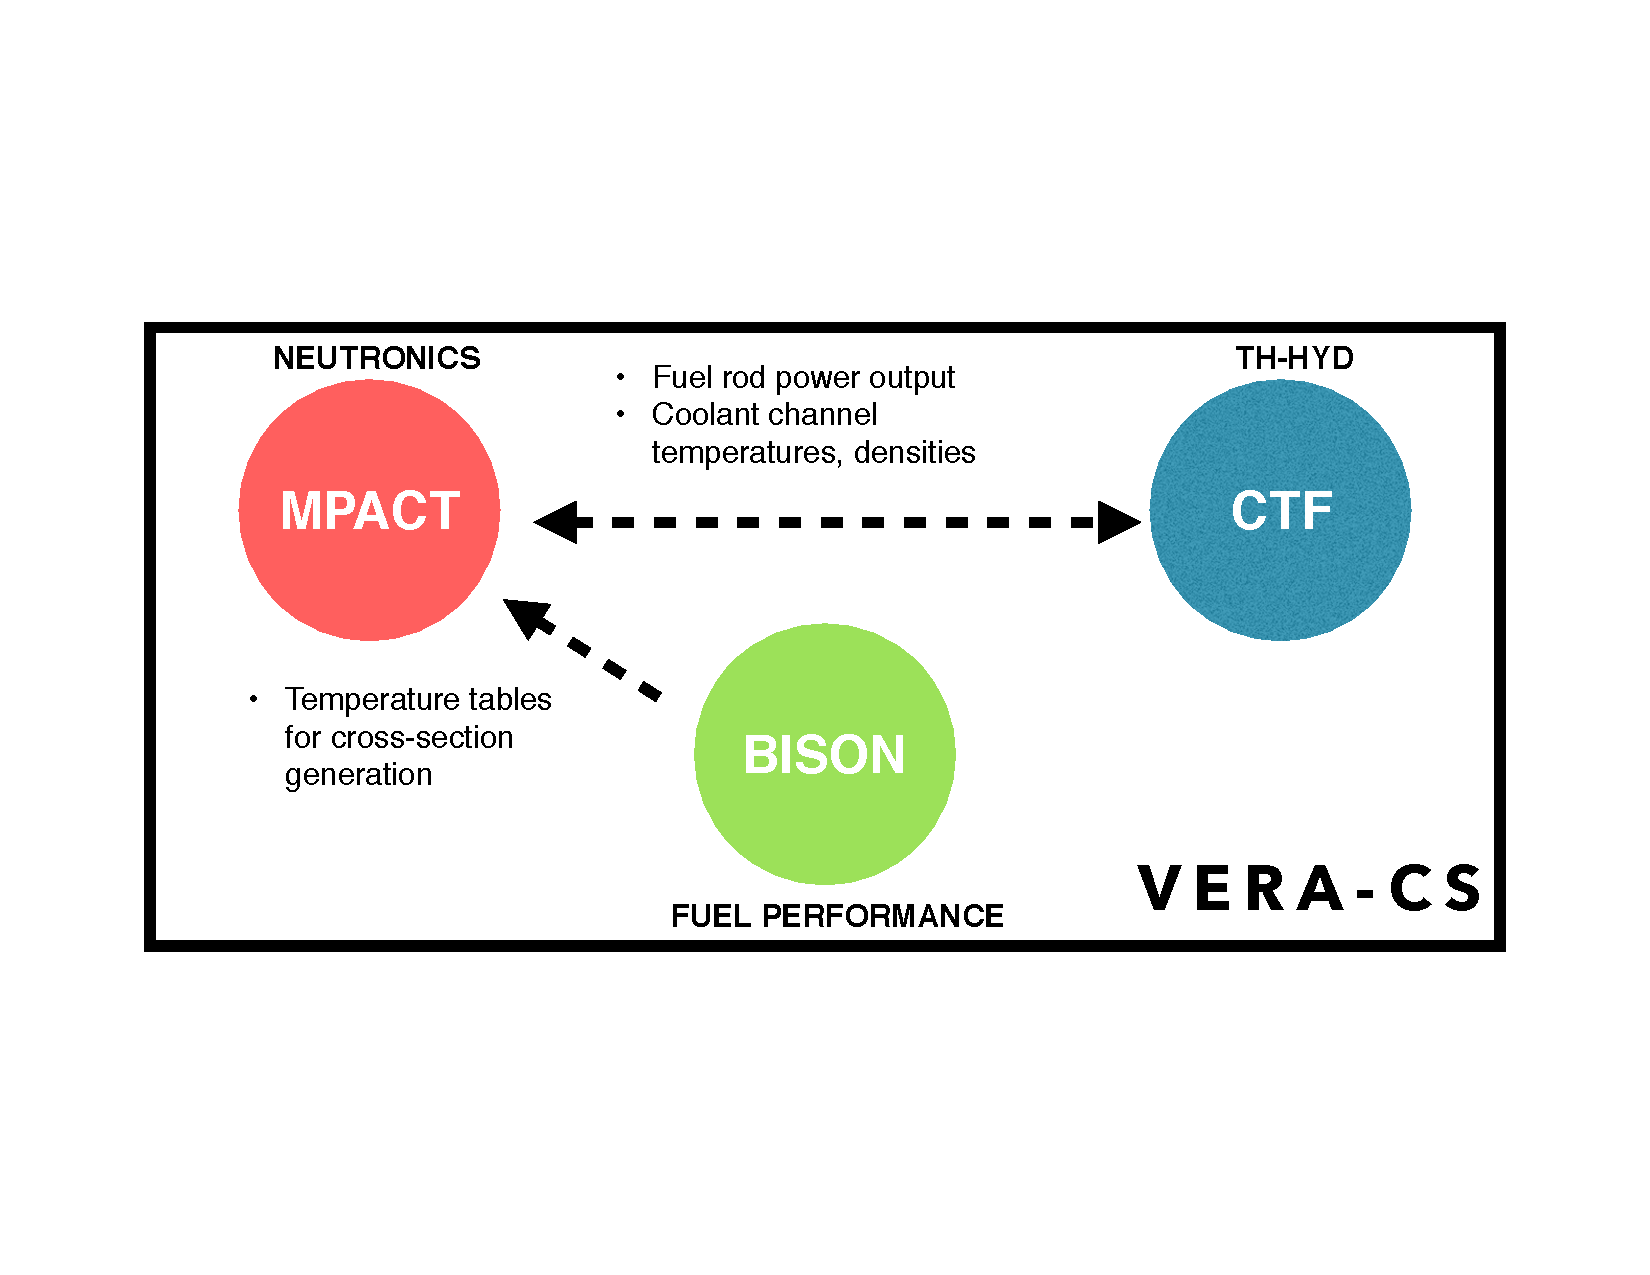
\includegraphics[width=0.5\linewidth,trim={2cm 5cm 2cm 5cm}]{./Figures/VERA-CS-Figure.pdf}
\end{center}
\caption{Primary physics simulator components of VERA-CS used in this work.}
\label{fig:workflow}
\end{figure} 

\subsubsection{MPACT}
MPACT is a neutron transport solver being developed by the \gls{UMich} and \gls{ORNL}. 
It provides pin-resolved flux and power distributions \cite{kochunas_overview_2013}. 
To solve three-dimensional (3D) problems, it employs a 2D/1D method, which decomposes the problem into a 1D axial stack of 2D radial planes \cite{zhu_assessment_2014}. 
These planes are then solved using Method of Characteristics (MOC). 
While there are a variety of axial solvers available, the Nodal Expansion Method (NEM)-simplified P3 (SP3) solver is the default, which wraps a one-node NEM kernel \cite{stimpson_axial_2014}. 
These 2D and 1D solvers are coupled together through transverse leakage to ensure neutron conservation, and they are accelerated using 3D \gls{CMFD}. 

\subsubsection{CTF}
CTF is a subchannel TH code being developed by \gls{ORNL} and \gls{NCSU} for LWR analysis \cite{avramova_ctf:_2009}. 
It simulates two-phase flow with a three-field representation (liquid, droplet, and vapor) assuming the liquid and droplet fields are in a dynamic equilibrium, leaving two energy conservation equations. 
CTF provides significantly higher resolution and physical detail than the internal TH solver in MPACT, thus requires longer execution times. 

\subsection{Work Flow and Modeling Strategy}

Several steps were involved in producing an accurate neutronic/thermal-hydraulics core model. 
Figure \ref{fig:method} displays the VERA-CS modeling stages used in this work.


\begin{figure}
\begin{center}
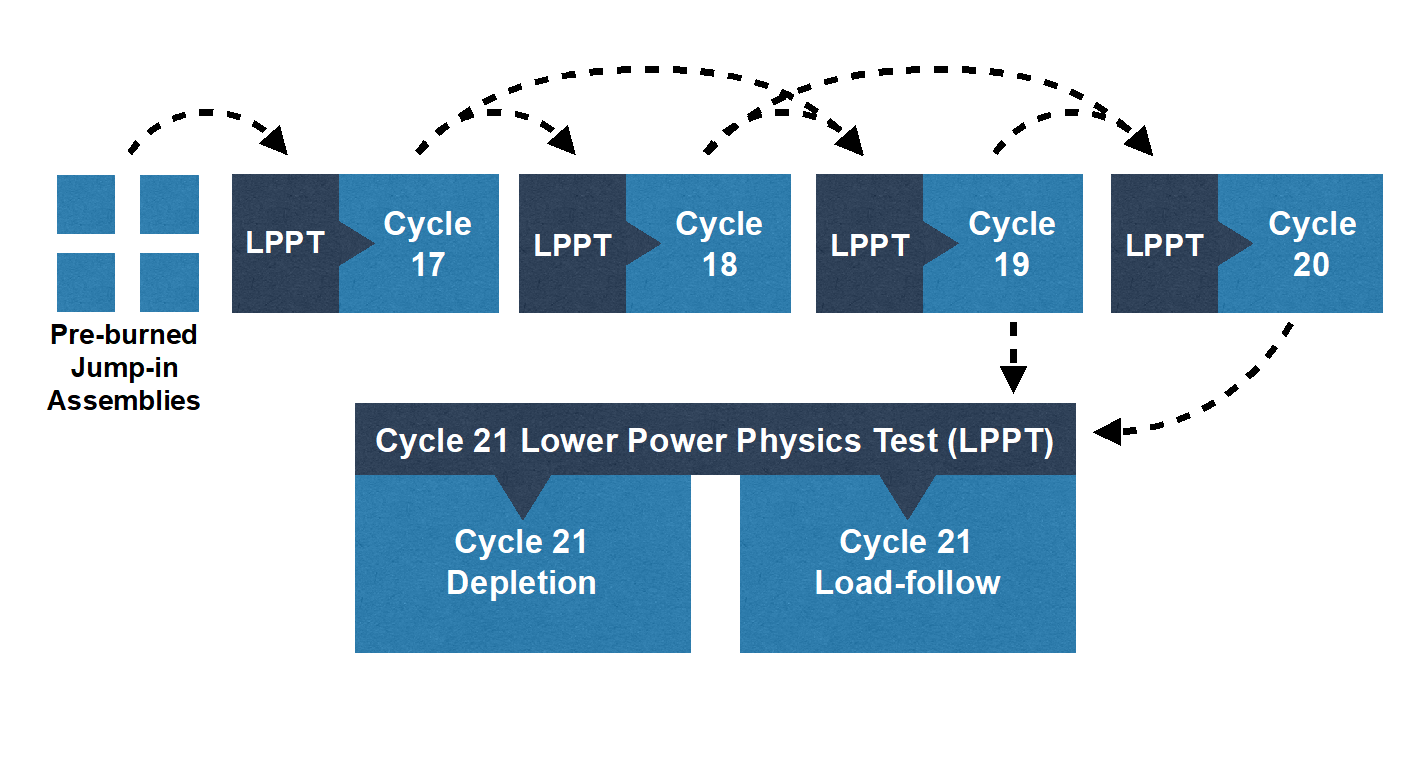
\includegraphics[width=0.5\linewidth]{./Figures/method.png}
\end{center}
\caption{Modeling strategy to simulate load follow in PWR1 cycle 21.}
\label{fig:method}
\end{figure} 

In most cases, each cycle includes assemblies from the previous two cycles, which necessitates a total of five cycles of depletion simulation to provide an accurate isotopic composition and power histories for the oldest assemblies present in cycle 21 (from cycle 19). 
Although it would be most accurate to start modeling from the \gls{BOL} of PWR1, this is computationally impractical. 
In this work, individual pre-burned assemblies were inserted into the cycle 17 core model through a "jump-in" strategy to approximate the shuffled assemblies present in cycle 17 (from cycle 15 and 16). 
These approximate assemblies are removed from the core by the start of cycle 19, which minimizes their effect on isotropic accuracy of our target cycle, cycle 21. 

Because of the difficulties in performing single assembly 3D depletion, special attention was paid to the exposure axial offset of each assembly at its desired burnup. 
During the project it was determined that the exposure axial offset needs to be close to zero to prevent an unrealistic power axial offset from occurring in cycle 17. 
In order to approximate cycle 15 and 16 assemblies as closely as possible, a total of 7 assembly types were burned to 15 target burnups. 
These 15 assemblies were then inserted into the proper position in cycle 17, based on the core loading scheme.


%%%%%%%%%%%%%%%%%%%%%%%%%%%%%%%%%%%%%%%%%%%%%%%%%%%%%%%%%
\section{VERA-CS Results}
%%%%%%%%%%%%%%%%%%%%%%%%%%%%%%%%%%%%%%%%%%%%%%%%%%%%%%%%%

\subsection{Low Power Physics Testing}
Before the cycle depletion was simulated, a \gls{LPPT} was conducted to validate the shuffling scheme, as shown in Figure \ref{fig:method}.
The \gls{LPPT}s included a critical boron search, an \gls{ITC} test and a \gls{CRW} test. 
The \gls{ITC} test was conducted by varying the temperature of the fuel and moderator by $\pm$4 $^\circ$F. 
The change in reactivity was then used to determine the \gls{ITC}. 
The \gls{CRW} tests were performed using a \gls{DRWM} technique, where each control rod bank was individually inserted into the core and the change in reactivity was used to determine the control bank's worth. 
The comparison of the calculated critical boron, \gls{ITC} and \gls{CRW} to their measured value is shown in Table \ref{tab:cb}, and Figure \ref{fig:crw}, respectively. 
It is observed that MPACT accurately predicts the measured critical boron value from cycle 19 onward.
The \gls{ITC} predictions are within 2 pcm for all cycles, which is within a reasonable margin of error.
In addition, it is observed that the predicted \gls{CRW} values are all within $\pm6$ \%.
It is observed that from cycle 19 onward, the \gls{CRW} values for the different control banks tend to become more irregular.
This behavior is undesired and requires further investigation.
Regardless, the total predicted control rod worth was within 1 \% for cycle 19, 20 and 21, which is within measurement uncertainties. 
It should be noted that some of the large relative errors observed in the control rod worth comparisons are a results of low measured rod worth. 
Based on these comparisons, it is concluded that any error introduced by the individually burned assemblies inserted into cycle 17 is eliminated by cycle 19, which shows an excellent agreement with the measured values. 

\begin{table}
\caption{Low Power Physics Results}
\label{tab:cb}
\begin{center}
\begin{tabular}[!t]{ccc}
\textbf{Cycle}      & \textbf{Critical Boron}   & \textbf{Isothermal Temp. Coeff.}      \\
           & \textbf{Difference [ppm]} & \textbf{Difference [pcm/$^{\circ}$F]}  \\ 
17 & -42 & -0.6     \\
18 & 44  & -1.4     \\
19 & 1   & -1.7     \\
20 & 3   & -0.83    \\
21 & -10 &  0.4     \\
\end{tabular}
\end{center}
\end{table}



\begin{figure}
\begin{center}
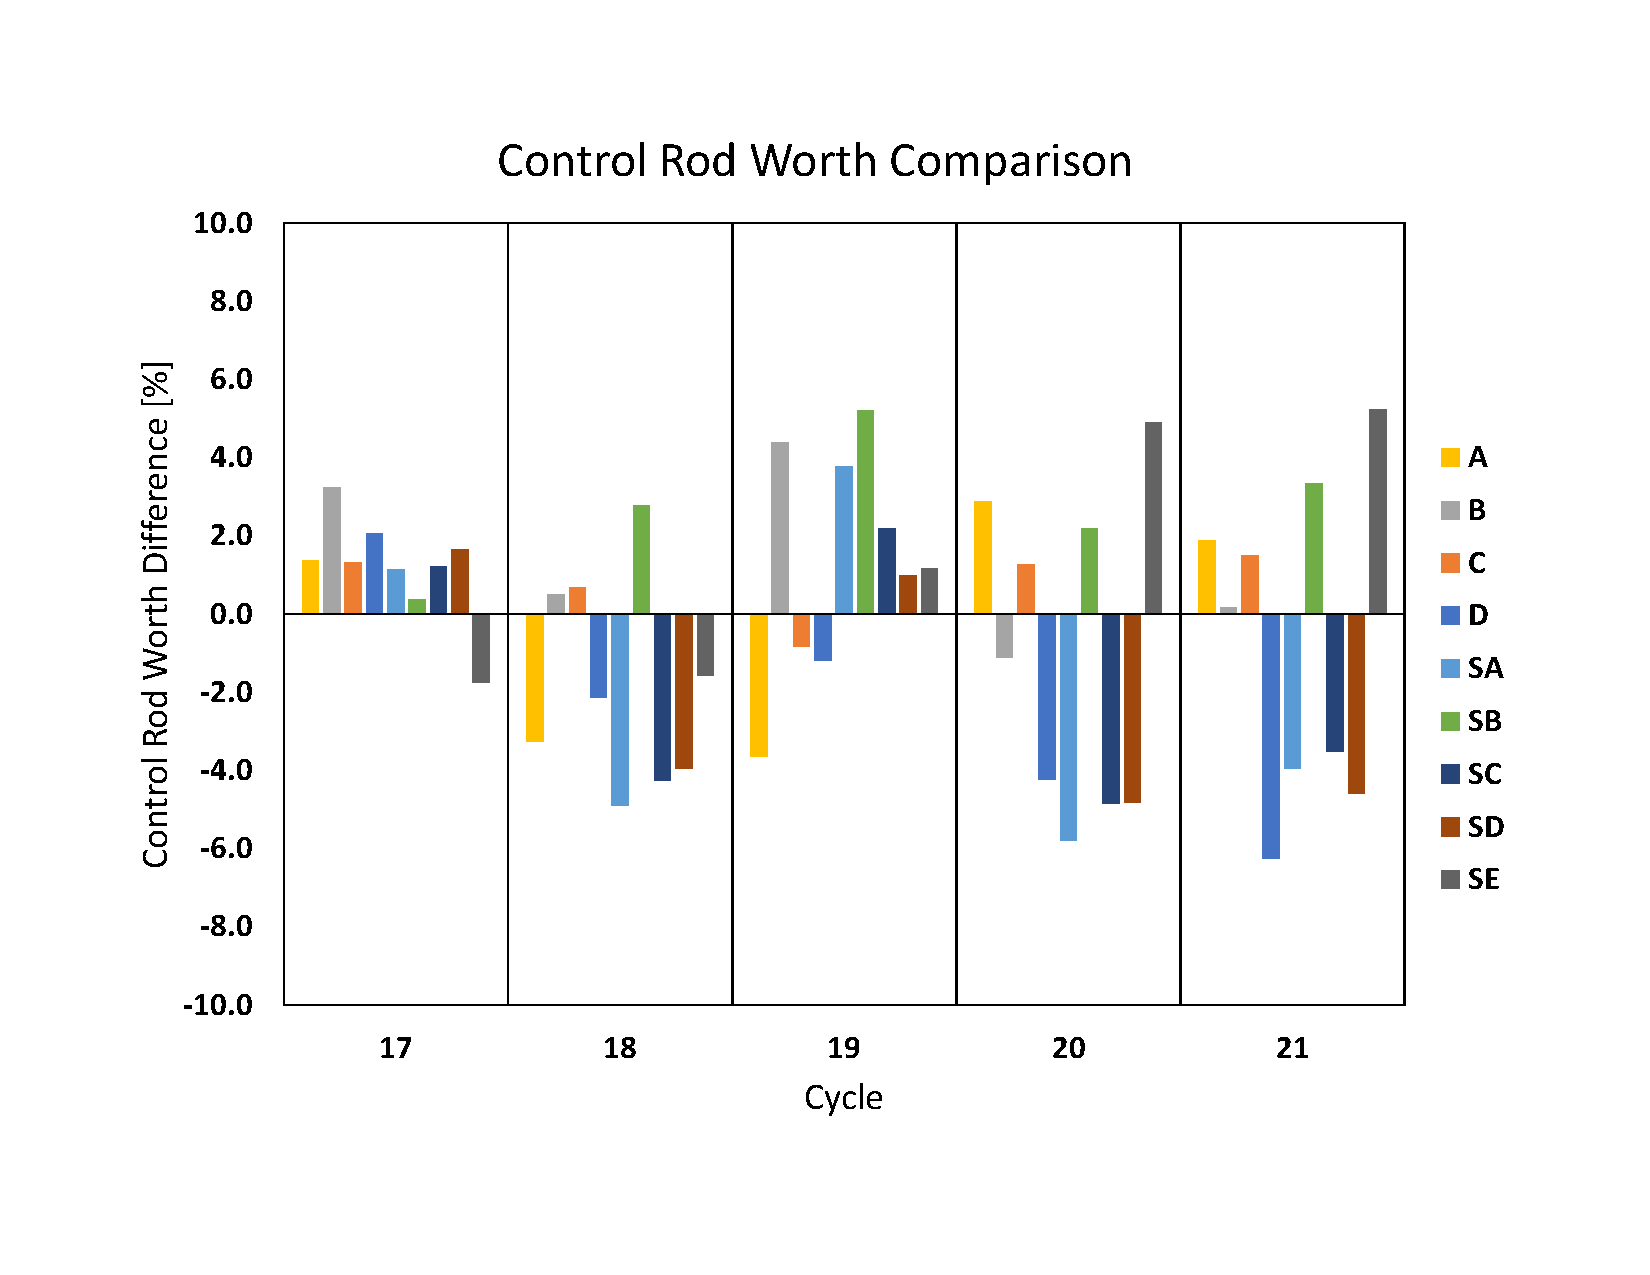
\includegraphics[trim={0 2cm 0 2cm},clip,width=0.85\linewidth]{./Figures/crw_diff.pdf}
\end{center}
\caption{Comparison of control rod worth of all 9 rod banks at HZP.}
\label{fig:crw}
\end{figure} 

\subsection{Cycle Depletion}
After the shuffling scheme for each cycle had been validated, cycle depletion was simulated from the \gls{BOC} to the \gls{EOC}, with special attention paid to the shutdown time between \gls{EOC} and \gls{BOC} of the next cycle to ensure accurate fission product decay between cycles. 
As the fuel is depleted over a reactor cycle, the boron concentration in the coolant is reduced via dilution to maintain criticality. 
In addition to the boron concentration being diluted over the length of the cycle, the weight percent of $^{10}$B is also reduced. 
This reduction is a result of boron depletion and is known to increase the critical boron concentration during the later dates of the cycle. 
MPACT can account for boron depletion through explicit input of $^{10}$B enrichment, but this requires measurements of the $^{10}$B concentration before the simulation can be performed.
As an alternative, the simulations is conducted with a constant $^{10}$B enrichment of 19.9 w/o and the measured critical boron is corrected using the measured $^{10}$B enrichment.
\begin{figure}
\begin{center}
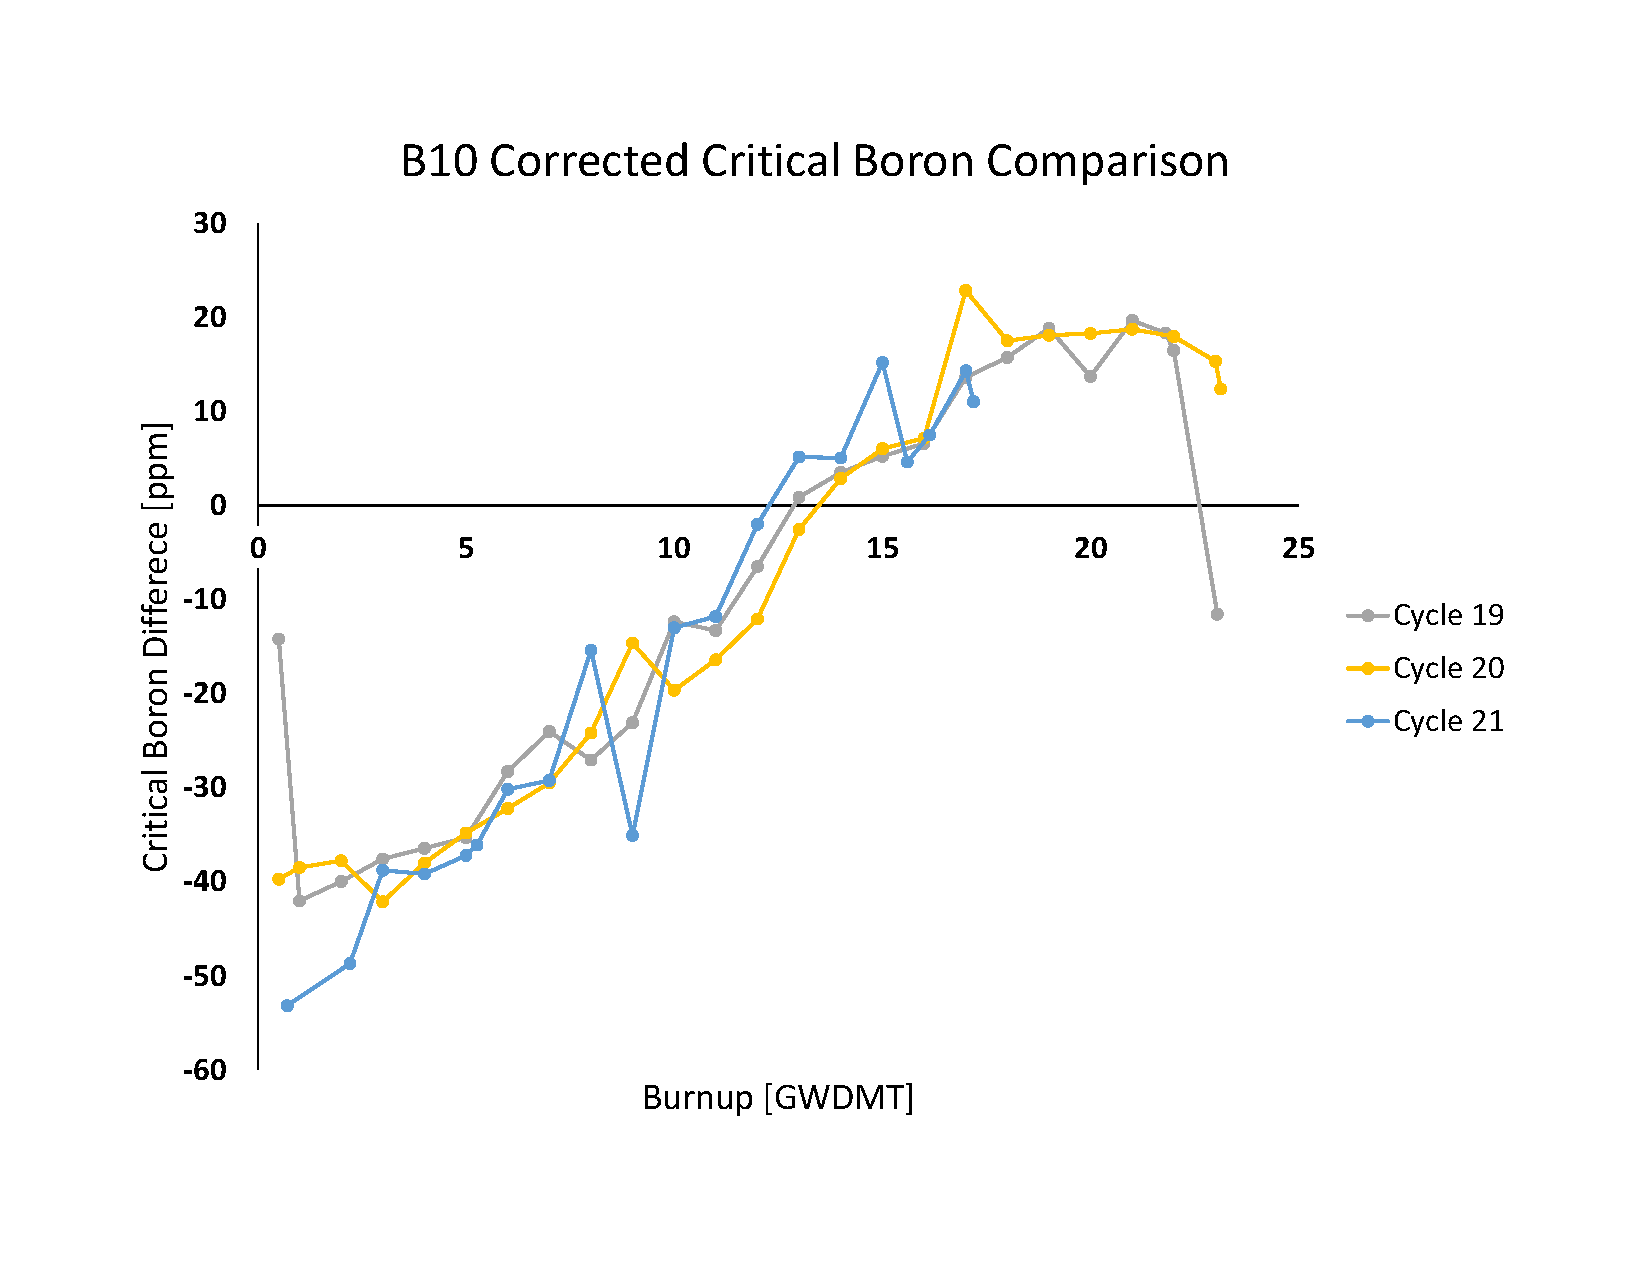
\includegraphics[trim={0 2cm 0 3.1cm},clip,width=0.85\linewidth]{./Figures/corr_b.pdf}
\end{center}
\caption{Comparison of simulated to the measured critical boron concentrations.}
\label{fig:cor_b}
\end{figure} 

The measured boron concentrations were used to establish the accuracy of the core reactivity vs. fuel burnup. 
The boron ``letdown" is compared for cycles 19-21 in Figure \ref{fig:cor_b}. 
Figure \ref{fig:cor_b} contains a comparison of the corrected measured boron concentration with the MPACT simulation. 
As shown in Figure \ref{fig:cor_b}, the difference between corrected measured and simulated critical boron concentration varies between -40 ppm at the beginning of cycle to +20 ppm at the end of the cycle. 
The cause of this reactivity swing is believed to be the temperature tables used to determine the fuel's temperature as a function of burnup and linear heat rate.
These tables are not used during \gls{HZP} calculations, which show good agreement to the measured values, and are constant for all three cycles, which have very consistent discrepancies.
Regardless, the difference is within 50 ppm for each cycle depletion, which is considered sufficiently accurate.

%%%%%%%%%%%%%%%%%%%%%%%%%%%%%%%%%%%%%%%%%%%%%%%%%%%%%%%%%
\section{Load-Follow Operation}
%%%%%%%%%%%%%%%%%%%%%%%%%%%%%%%%%%%%%%%%%%%%%%%%%%%%%%%%%

After further review of the test stand's depletion results, it was determined that the \gls{UIUC} model of PWR1 displayed sufficient agreement with plant measured data. 
In addition to cycle depletion, hourly depletion simulations were performed for the first month of plant operation.
During this time period, a total of 5 power maneuvers were performed, each varying the plant's power output between 100\% and 70\%.
During the \gls{VERACS} simulations the exact reactor power, control rod position, and moderator inlet temperature were modeled using hourly depletion steps.
A graphical representation of the power histories, can be found in Figure \ref{fig:lf_his0}.

\begin{figure}[h]
\begin{center}
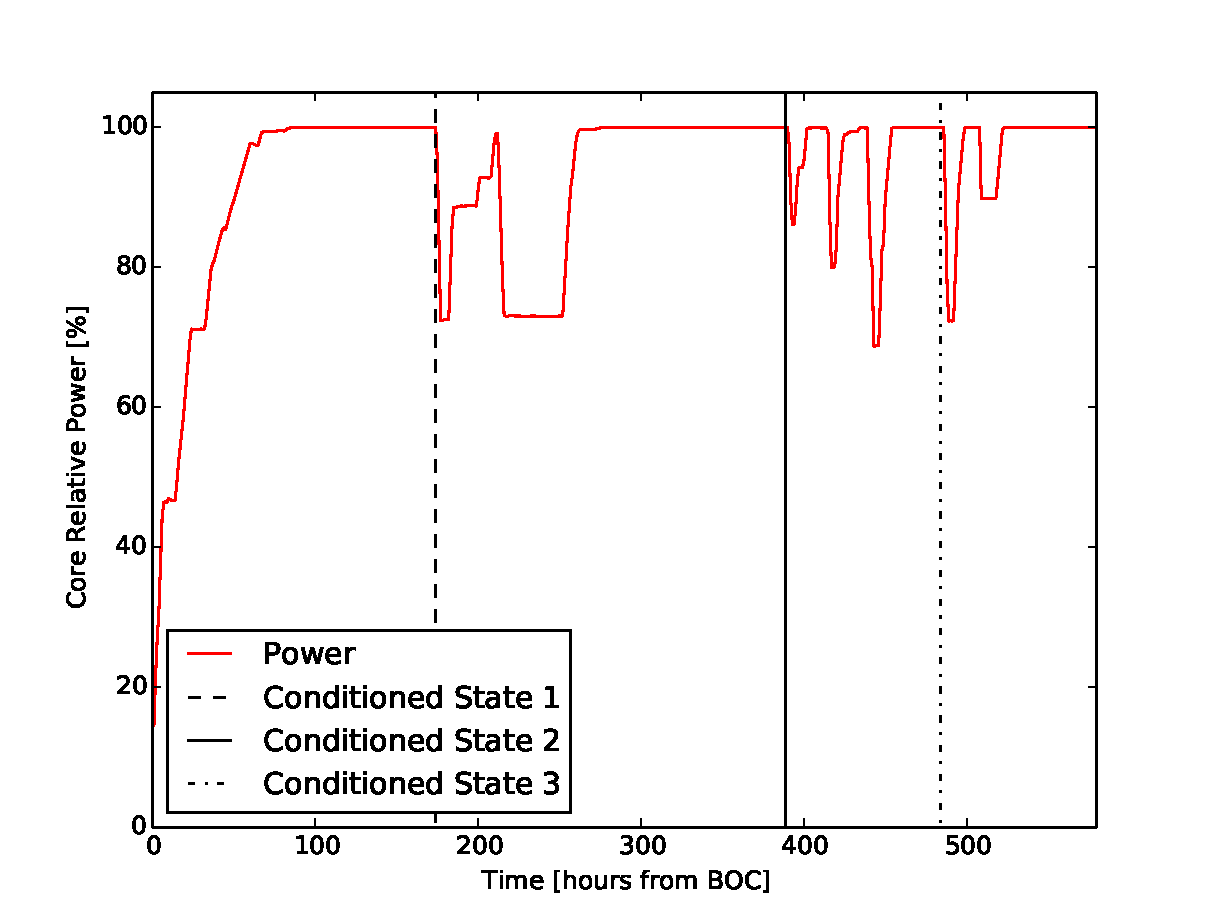
\includegraphics[width=3in]{./Figures/M_power_his.pdf} 
\end{center}
\caption{PWR1 power history during the first 20 days of plant operation}
\label{fig:lf_his0}
\end{figure}


\begin{figure}[h]
\begin{center}
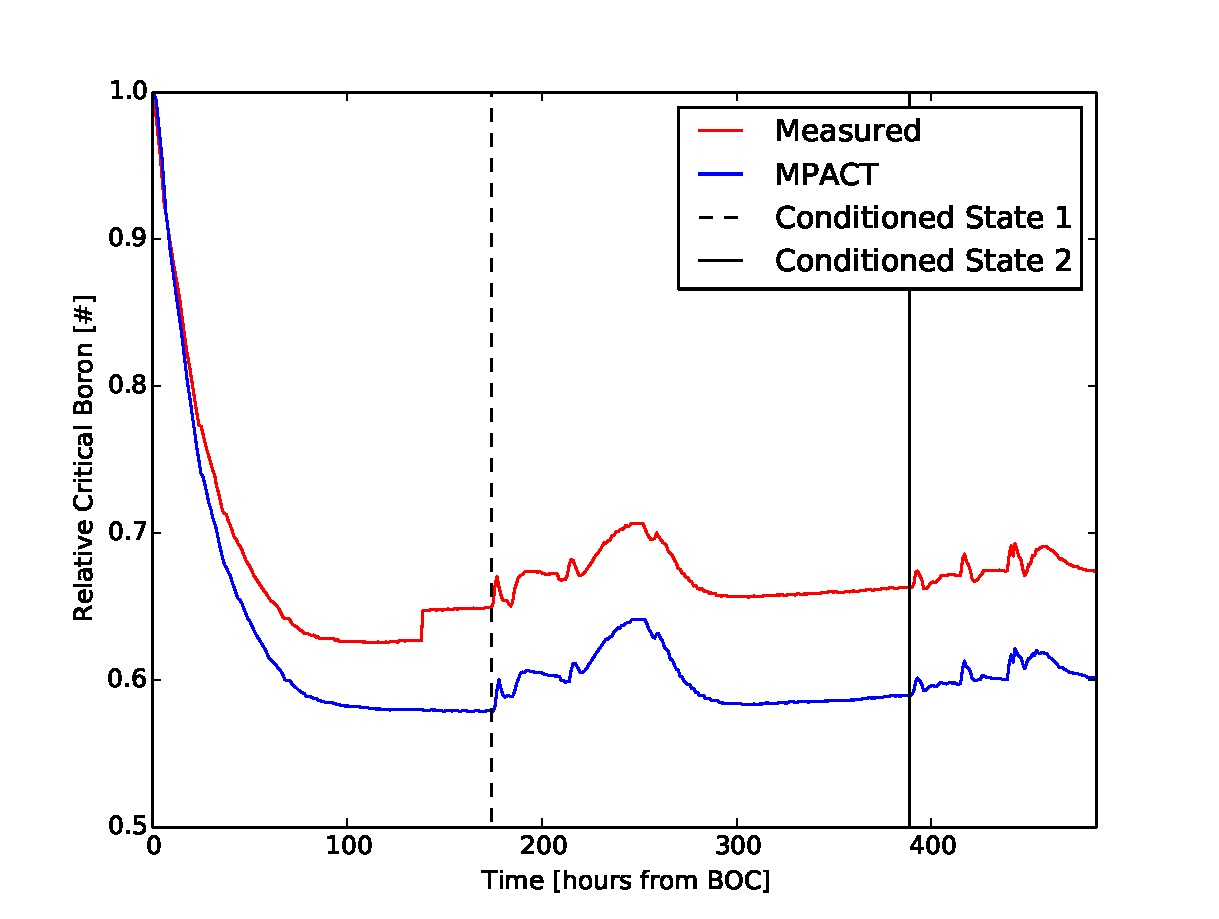
\includegraphics[height=4in]{./Figures/M_boron.pdf} 
\end{center}
\caption{PWR1 hourly critical boron concentration  comparison  during the first 20 days of plant operation}
\label{fig:lf_his2}
\end{figure}

\begin{figure}[h]
\begin{center}
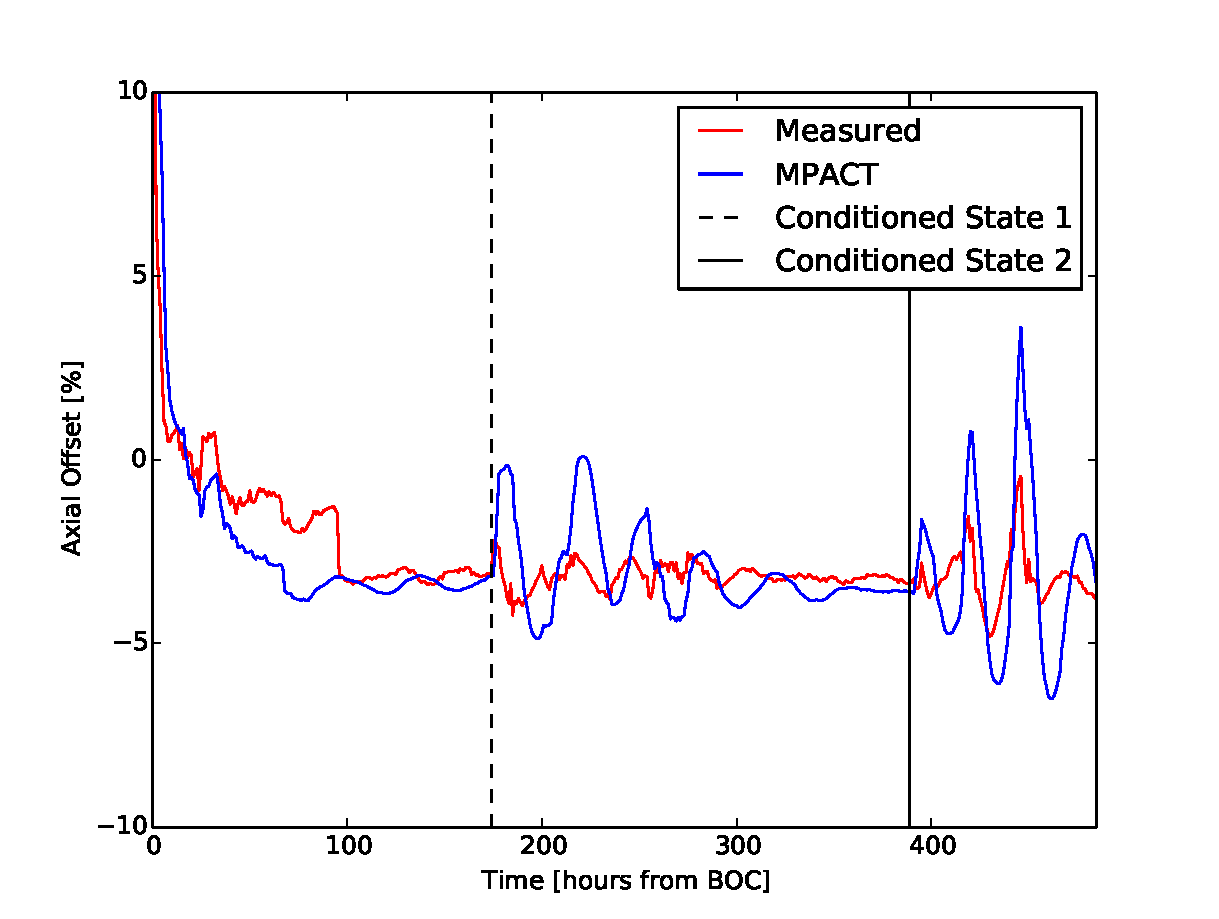
\includegraphics[height=4in]{./Figures/M_AO.pdf} 
\end{center}
\caption{PWR1 hourly \gls{AO} comparison during the first 20 days of plant operation}
\label{fig:lf_his1}
\end{figure}

In order to validate the MPACT simulation, the critical boron was calculated during the load-follow simulation. 
The MPACT predicted critical boron and \gls{AO} were then compared to the estimated critical boron and \gls{AO} provided by the industry partner.
Unfortunately, the estimated critical boron was obtained using the core monitoring system, which was shown to have incorrect critical boron concentrations before a kbias was applied. 
As a result, a direct comparison of the critical boron was not performed, instead a comparison of the critical boron response immediately following a kbias was used to validate the prediction.
It is observed in Figure \ref{fig:lf_his2} that the MPACT predict boron response shows excellent agreement with the core monitoring system boron response during the load-follow power maneuvers at \gls{BOC}.
The comparison of the MPACT predict \gls{AO} and the plant estimated \gls{AO}, shown in Figure \ref{fig:lf_his1}, allows for several conclusions to be drawn about the MPACT simulation.
At times when power is decreased, both the MPACT and plant \gls{AO} are observed to increase.
This behavior is expected as the moderator temperature coefficient should push power towards the top of the core as power is decreased.
Unfortunately, the MPACT predictions overestimate the magnitude of the positive swing.
This overestimation could be a result of the temperature tables used in the simulation or the underi predicted control bank worth.
Additionally, sinusoidal oscillations in the MPACT \gls{AO} are observed during times of constant power following a power maneuver.
These oscillations are not observed in the plant data but their magnitude is negligible as they are less then 1 \% from peak to peak.
  
Further investigation is required to reduce the observed discrepancies.
It is important to note, plant operators are able to modify the control rod position in real time to control the \gls{AO}, the data used to create the MPACT model is based on plant configurations on the hour and contains no sub information.
In general it can be concluded that the MPACT predictions are within plant measurement uncertainties.
Therefore, the results of these simulations, linear heat rates and cladding surface temperatures, can be used as the boundary conditions in fuel performance calculations.
The detailed pin level data that is available from the \gls{VERACS} results allows for reduced uncertainties in the fuel performance boundary conditions leading to more accurate predictions of peak cladding hoop stresses within a pin.

%%%%%%%%%%%%%%%%%%%%%%%%%%%%%%%%%%%%%%%%%%%%%%%%%%%%%%%%%
%%%%%%%%%%%%%%%%%%%%%%%%%%%%%%%%%%%%%%%%%%%%%%%%%%%%%%%%%
\chapter{Methodology}
%%%%%%%%%%%%%%%%%%%%%%%%%%%%%%%%%%%%%%%%%%%%%%%%%%%%%%%%%
%%%%%%%%%%%%%%%%%%%%%%%%%%%%%%%%%%%%%%%%%%%%%%%%%%%%%%%%%
The main focus of this work is to predict the limiting pin within a commercial \gls{PWR} during load-follow power maneuvers.
Due to the stochastic nature of \gls{PCI} induced fuel failure and the randomness of pellet defects throughout the core, determining a single pin out of the approximately 60,000 present is unrealistic.
Instead, the top 1000 most likely limiting fuel pins are selected to be analyzed using the three step process outlined by Lyon et al. \cite{lyon_pci_2009}.
Similar to the assembly based screening process developed by Kennard et al., the pin based screening process will look at characteristics indicating the fuel's conditioning.
In order to determine the validitiy of this screening process, all fuel pins contained within the quarter core \gls{VERACS} model will simulated using the BISON fuel performance code.
In the following sections the procedure for selecting the 1000 fuel pins and a description of the BISON fuel performance code are presented.

%%%%%%%%%%%%%%%%%%%%%%%%%%%%%%%%%%%%%%%%%%%%%%%%%%%%%%%%%
\section{MPACT Screening Process}
%%%%%%%%%%%%%%%%%%%%%%%%%%%%%%%%%%%%%%%%%%%%%%%%%%%%%%%%%

As described in \cite{capps_evaluation_2016,kennard_pci_2016}, fuel rod response to a change in power is a function of the fuel rod's conditioning. 
In the presence of significant fuel exposure and/or operation at a high linear heat rate, the strongest indicator of elevated failure risk is a sudden increase above the conditioned power.
To quantify the risk of \gls{PCI} induced fuel failure, a weighted change in linear heat rate, $R$, is calculated for each fuel pin,
\begin{equation}
R_{i,j,k}^{t} = \frac{\left( lhr_{i,j,k}^t-lhr_{i,j,k}^{t_{con}}\right)}{lhr_{i,j,k}^{t_{con}}} b_{i,j,k}^t \cdot lhr_{i,j,k}^{t}
\end{equation}
where $lhr$ and $b$ are the MPACT predicted linear heat rate and burnup, respectively, for fuel pin ($i$,$j$) at the axial location $k$ and time $t$.
For cycle start-up ramps, the conditioned power is taken as the linear heat rate a shuffled fuel rod experienced at the end of the previous cycle, $lhr_{i_{prev},j_{prev},k}^{t_{end}}$.
During a load-follow operation, the conditioned power is taken to be the linear heat rate experienced while operating at full power before the maneuver began, $lhr_{i,j,k}^{t_{con}}$.
For example, in Figure \ref{fig:lf_his0} the linear heat rates calculated at hour 175 are assumed to be the conditioned linear heat rates for the following two power maneuvers, $t_{con}=175$. 

The weighted change in linear heat rate accounts for all parameters that effect \gls{PCI}.
The relative change from conditioned power determines if elevated stress is being applied on the cladding's inner surface.
Positive changes suggest that the fuel pellet has expanded, applying a tensile hoop stress on the cladding.
Negative changes suggest that the fuel pellet has contracted and fuel failure is unlikely.
In the presence of a closed gap, the thermal expansion of the fuel pellet will cause elevated stresses on the cladding.
Due to the fact that gap width is a complex function of power history, the fuel's linear heat rate and burnup are used to determine the likelihood that the gap has closed.
When the fuel's burnup and linear heat rate are high it is unlikely that the gap is open.
Additionally, the fuel's burnup suggests the presence of fission products on the clads inner surface.
When multiplied, these three parameters indicate the fuel rods that are under elevated stress and have the potential to fail due to \gls{PCI}.

An important factor to consider is the effect prolonged load follow operation will have on the fuel's response.
The degradation of the conditioned power, or the fuel deconditioning, is not well understood.
The primary change in the fuel rod during deconditioning is a reduction of the cladding inner diameter.
Cladding creep down, which is dependent on temperature, irradiation history, and applied stress, is the primary mechanism responsible for the reduction.  
For cycle start-up ramps, where the cladding and fuel rods are stored at reduced temperatures, deconditioning can be neglected. %maybe have a reference for this
On the other hand during extended periods of low power operation where the cladding is exposed to elevated temperatures and stresses, it is possible that the cladding creep rate is not negligible.
Therefore the conditioned power level could be a function of time spent at reduced power.
A previous study \cite{galrtner_survey_1987} suggests that multiple power ramps have no effect on the conditioned power level of the fuel rod.  
However, the results presented by Stimpson \cite{stimpson_demonstration_2017} on continuous load-following for a single fuel pin suggest that changes in burnup have a strong effect on the maximum clad hoop stress.
This effect is taken into consideration by the burnup factor in the weighted change in linear heat rate.
As a result, it is assumed that fuel deconditioning does not occur during load-follow operation.


%%%%%%%%%%%%%%%%%%%%%%%%%%%%%%%%%%%%%%%%%%%%%%%%%%%%%%%%%
\section{BISON}
%%%%%%%%%%%%%%%%%%%%%%%%%%%%%%%%%%%%%%%%%%%%%%%%%%%%%%%%%

The BISON fuel performance code is developed by \gls{INL} to provide single-rod fuel performance modeling capability to assess best-estimate values of design and safety criteria. 
BISON is built on \gls{INL}'s \gls{MOOSE} package \cite{gaston_moose:_2009}, which uses the finite element method for geometric representation and a Jacobian Free Newton-Krylov (JFNK) scheme to solve systems of partial differential equations \cite{williamson_multidimensional_2012}. 
Three primary differential equations are implemented in BISON to determine the response of a nuclear fuel rod to changes in  power.
These equations describe the conservation of energy, momentum, and species, which are defined by,
\begin{equation} \label{eqn:bis_eng}
\rho C_p \frac{\partial T}{\partial t} + \nabla \cdot \vec{q} - e_f \dot{F} =0
\end{equation} 
\begin{equation} \label{eqn:bis_mom}
\nabla \cdot \vec{\sigma} + \rho \vec{f} =0
\end{equation} 
\begin{equation} \label{eqn:bis_spec}
\frac{\partial C}{\partial t} + \nabla \cdot \vec{J} +\lambda C - S =0.
\end{equation} 
$\rho$, $C_p$ and $T$ respectively describe the density, specific heat and temperature of a material subject to a volumetric heat source, described by $e_f$, the energy released per fission, and $\dot{F}$ the volumetric fission rate.
$\sigma$ describes the Cauchy stress tensor under static equilibrium and a specific body force, $\vec{f}$.
$C$, $\lambda$, and $S$ are the concentration, decay constant and volumetric source of a particular isotope.
The implementation of these equations allows for non-linear kinematics and non-linear material behavior.
This accounts for the temperature dependent thermal and mechanical properties of the nuclear fuel and incorporates the effects of material creep and plasticity.
Further information on the implementation of material properties, including thermal conductivity, fuel swelling, creep and fission gas release, can be found in \cite{williamson_validating_2016,hales_bison_2015}.

In order to validate the predicted fuel response, a suite of experimental fuel rods have been simulated using BISON.
Measured quantities including fuel centerline temperature, volume of gas released and pin diameter, were compared at \gls{BOL} and \gls{EOL} \cite{williamson_validating_2016}.
It was consistently shown that BISON is capable of predicting fuel centerline temperatures within 10\% of the measured value.
Although a 10\% error at elevated fuel temperatures, $\pm$90 $^\circ$C at 900 $^\circ$C, is significant, the measured linear heat rate of the experimental conditions is only accurate within 6\%. 
This implies that a portion of the error can be contributed to measurement uncertainties, thus the 10\% error is considered quite accurate.
Fission gas release predictions are typically within a factor of two of the measured values.
This agreement is considered within the range of measurement error and is common among many fuel performance simulators.
Although fission gas release and fuel temperature show acceptable agreement with measured quantities, rod diameter tends to be under predicted at \gls{BOL} and over predicted at \gls{EOL}.
This discrepancy is believed to be caused by a lack of a relocation recovery model.
Nonetheless, BISON has been shown to capture complex thermo-mechanical behavior such as PCI failures in PWRs \cite{montgomery_advanced_2014,capps_pci_2017}.

\gls{CASL} has developed a methodology to perform fuel performance simulations for all fuel rods simulated using \gls{VERACS}.
The methodology relies on a template input file and a parser.
Fuel performance calculations can be run coupled with \gls{VERACS}, inline with \gls{VERACS} or standalone.
In this work, fuel performance calculations are run standalone using a 1.5D template.
This means that the linear heat rate and coolant temperature predicted using \gls{VERACS} are applied as boundary conditions for the BISON calculations.
Unlike an RZ simulation, the 1.5D template neglects axial conduction within the fuel rod.
Rather, a stack of smeared 1D pellets are coupled using a common plenum pressure.  
This geometric configuration has been shown to significantly reduce the computational time required for each power ramp \cite{gardner_review_2017}.
Due to the fact that the RZ simulation commonly used for standalone BISON calculations uses a smeared pellet mesh, where individual pellets are not explicitly modeled, the 1.5D results are expected to have consistent predictions.
In a standard \gls{PCI} screening process, the results of RZ fuel performance simulation are used to select the axial location for a R-$\theta$ simulation.
Therefore, with consistent boundary conditions between the RZ and 1.5D simulations, the reduced run time allows for additional fuel performance calculations to be conducted.



%%%%%%%%%%%%%%%%%%%%%%%%%%%%%%%%%%%%%%%%%%%%%%%%%%%%%%%%%



%%%%%%%%%%%%%%%%%%%%%%%%%%%%%%%%%%%%%%%%%%%%%%%%%%%%%%%%%
\chapter{Results and Discussion}
%%%%%%%%%%%%%%%%%%%%%%%%%%%%%%%%%%%%%%%%%%%%%%%%%%%%%%%%%
%%%%%%%%%%%%%%%%%%%%%%%%%%%%%%%%%%%%%%%%%%%%%%%%%%%%%%%%%
Using the results of the load-follow and  cycle depletion simulations, stand-alone bison inputs were created for all fuel pins contained within cycle 21. 
These inputs modeled each pin's detailed power history, which accounted for core shuffling and cycle outages. 
%An example of a shuffled pins power history is shown in Figure \ref{fig:single_pin}, where the pin was present towards the center core during cycles 19 and 20, and was then moved to the periphery of the core during cycle 21. 
Of the 14,784 pins found in the quarter core model of cycle 21, all but approximately 150 fuel pins ran to completion.
After adjusting a radial biasing parameter within BISON, the 150 fuel pins ran to completion.
This biasing parameter causes the fuel pin's simulated power output to exceed the specified input power.
As a result, many of the parameters of interest, i.e. burnup, hoops stress, and gap thickness, may be overestimated.
This behavior has been reported to the BISON developers and requires further investigation. 
Nonetheless, the maximum clad hoop stress within these pins is similar to the surrounding fuel pins, allowing the screening process to be applicable.

In the remaining sections the BISON fuel performance and MPACT screening results for the first 20 days of operation are presented.
The BISON fuel performance results are broken into two sections, the initial power ramp, and the load-follow operation.
The MPACT screening results follow the same format but the initial power ramp is not considered. 
Core designers spend a significant amount of time looking at the initial power ramp, therefore it is assumed a well accepted screening process has already been developed for the initial ramp.

%%%%%%%%%%%%%%%%%%%%%%%%%%%%%%%%%%%%%%%%%%%%%%%%%%%%%%%%%
\section{BISON}
%%%%%%%%%%%%%%%%%%%%%%%%%%%%%%%%%%%%%%%%%%%%%%%%%%%%%%%%%

\subsection{Start-up Power Ramp}

Of the various quantities BISON calculates, two were chosen and plotted using VERAView \cite{lee_veraview_2016}.
Figures \ref{fig:bison_initial} through \ref{fig:bison_PR5} show the results for the maximum clad hoop stress (top), and the minimum fuel-clad thickness (bottom), at different times of operation. 
The BISON predicted clad damage index of all fuel pins during the load-follow power maneuvers was zero, for this reason it not displayed.
It should be noted that all of the figures only contain radial information as the collection of the three dimensional results is unavailable at this time. 
For reference, the relative core power is plotted to the right of each result, within this plot a red vertical line is used to indicate the time of the calculation.

From Figure \ref{fig:bison_initial}, useful information about the state of the fuel at \gls{BOC}  can be interpreted. 
The minimum distance between the cladding and fuel pellet, shown in the bottom of Figure \ref{fig:bison_initial}, allows for the determination of contact. 
It is observed that the majority of the burned fuel assemblies, shown in blue, have closed the gap. 
Some of the fuel rods on the periphery of the core show a slight gap, which can reduce the cladding hoops stress within those pins.
All fresh fuel assemblies have not closed the gap between the fuel and the clad, but thermal expansion has caused a reduction from the manufactured gap.

The maximum clad hoop stress during the initial power ramp was observed at full power.
This result is expected as the fuel temperature is proportional to the power level, therefore thermal expansion should be its greatest at full power.
Additionally, tensile hoop stress is only observed in shuffled fuel assemblies.
Due to the fact that fresh fuel assemblies have not closed the gap, the pressure differential between the coolant and the fill gas result in a compressive force, negative hoop stress, on the fresh fuel assemblies.
\gls{PCI} induced fuel failure is a result of a tensile force, therefore compressive forces can be neglected.
The maximum clad hoop stress was observed in assembly H-13, pin (5,13), circled in black in Figure \ref{fig:bison_initial}. 
At 94.1 MPa, the pressure exerted on the cladding is relatively low. 
The 5\% failure threshold determined by Capps et al. is 395 MPa for the two dimensional BISON rod, more then 3 times the pressure observed \cite{capps_pci_2017}.
It should also be considered that the 1.5D model neglects axial conduction, which will lead to an over prediction of the fuel temperature, causing elevated hoop stresses.
The low maximum clad hoop stress observed is anticipated as the initial power maneuver is carefully planned to minimize the risk of fuel failure.
The low pressure also indicates why the CDI was predicted to be zero, as BISON requires a 300 to 400 MPa hoop stress before clad damage can accumulate.



\subsection{Load-follow Power Maneuvers}

The BISON predicted maximum clad hoop stress for all load-follow power maneuvers are presented in the lower half of Figures \ref{fig:bison_PR1} through \ref{fig:bison_PR5}.
The maximum clad hoop stress  for each maneuver was observed to occur after the return to full power ramp.
When the maneuver was followed by a constant power hold, ramps 2 through 6, the maximum occurred approximately 8 hours after full power had been achieved.
This is believed to be caused by a xenon transient, which pushes the power away from the middle of the core.
As seen in Figure \ref{fig:lf_his1}, the simulation is out of phase and over predicting the plant response after most maneuvers.
Because the BISON calculations are based on the simulation results, the predicted fuel behavior is taken to be conservative.
Similar to the initial power ramp, tensile hoop stress is only observed in shuffled fuel assemblies for all power maneuvers simulated.
Due to the fact that only the first month of cycle operation was simulated, the fresh fuel assemblies do not experience a significant change in gap width after full power had been achieved.
Therefore the pressure differential is the dominant stress on the cladding and the fresh fuel assemblies can still be neglected.

The maximum clad hoop stress for each power maneuver is listed in Table \ref{tab:MHS} and circled in black in Figures \ref{fig:bison_PR1} through \ref{fig:bison_PR5}. 
Based on the figures, all power maneuvers appear to have similar effects on the core after a return to full power.
The effect load-follow power maneuvers has on the cladding stress is unclear this early in the cycle.
There does not appear to be a correlation between the characteristics of the ramps and the hoop stress they impose on the cladding.
Power ramp 2 had a similar power decrease and return to full power time as power ramp 5, but had a much longer hold time.
Both maneuvers show very similar maximum hoop stress suggesting that hold time does not have a strong effect.
This observation supports the assumptions that deconditioning can be neglected for load-follow power maneuvers, at least on the hour time scale.
Power ramps 1 and 5 have similar power decreases and hold times, but the ramp 1 returns to full power much slower.
The maximum hoop stress in both ramps is similar, suggesting that intermediate power holds due not appear to have as strong an effect on the maximum hoop stress as they during the initial start-up ramp.
Additionally, no correlation is observed between the power decrease and maximum hoop stress, as ramps 3 and 5 have similar hoop stresses.

The current trend in the maximum hoop stress after the initial start-up is proportional with the cycle exposure.
It can be assumed that this trend is likely to continue as the cycle continues but the redistribution of power in the core could result in asymptotic behavior.
Further investigation is required to determine the effect load-follow power maneuvers have towards the end of a cycle.
Nonetheless, cladding hoop stresses in the range of 95 MPa are well below the 5\% failure threshold and do not indicate a significant risk of early cycle load-follow power maneuvers. 

\begin{table}
\caption{Maximum clad hoop stress for each load-follow power maneuver}
\label{tab:MHS}
\begin{center}
\scalebox{0.75}{
\begin{tabular}[!t]{lcccccc}
\textbf{Power Ramp} & \textbf{Time}         & \textbf{Power Level}         & \textbf{Hold Time}         & \textbf{Return to Full}     & \textbf{Pin Position} & \textbf{Hoop Stress}  \\
                    & \textbf{[hours]}      & \textbf{[\%]}                & \textbf{[hours]}           & \textbf{Power time [Hours]} &                       & \textbf{[MPa]} \\
0 & 80  & N/A  & N/A  & 80* & H-13 (05,13)   & 94.1     \\
1 & 214 & 71.5 & 5    & 27* & C-08 (13,13)   & 87.4     \\
2 & 273 & 73   & 36   & 9   & C-08 (13,13)   & 89.5     \\
3 & 412 & 86   & 3    & 8*  & C-08 (13,05)   & 91.7     \\
4 & 437 & 80   & 3    & 7   & C-08 (13,05)   & 93.5     \\
5 & 458 & 70   & 3    & 8   & C-08 (13,05)   & 93.7     \\
\multicolumn{6}{l}{* Contains intermediate power holds}
\end{tabular}}
\end{center}
\end{table}

\begin{landscape}
\begin{figure}[h]
\begin{tabular}{c}
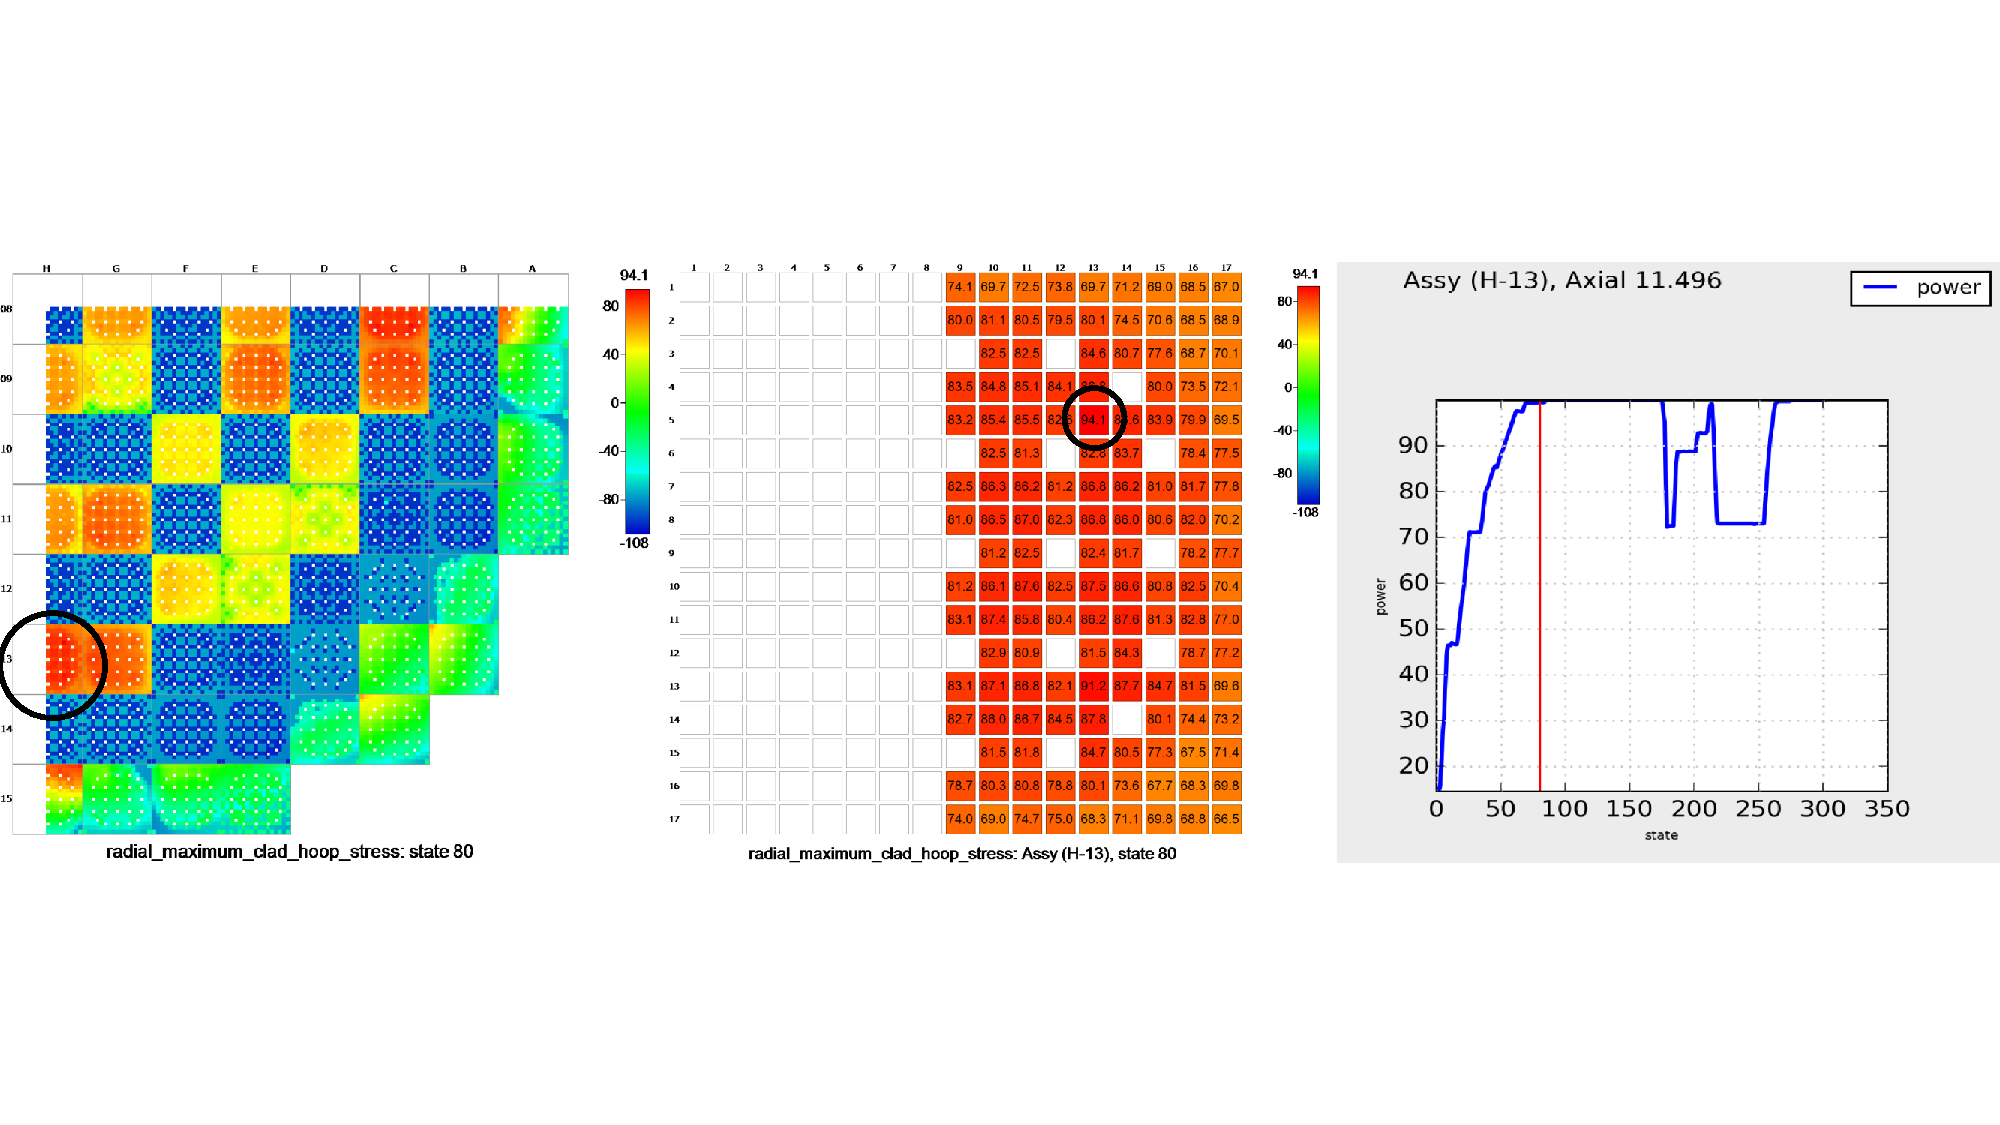
\includegraphics[trim={0 4cm 0 4cm},clip,width=\linewidth]{./Figures/bison_res/IPR_MCHS.pdf} \\
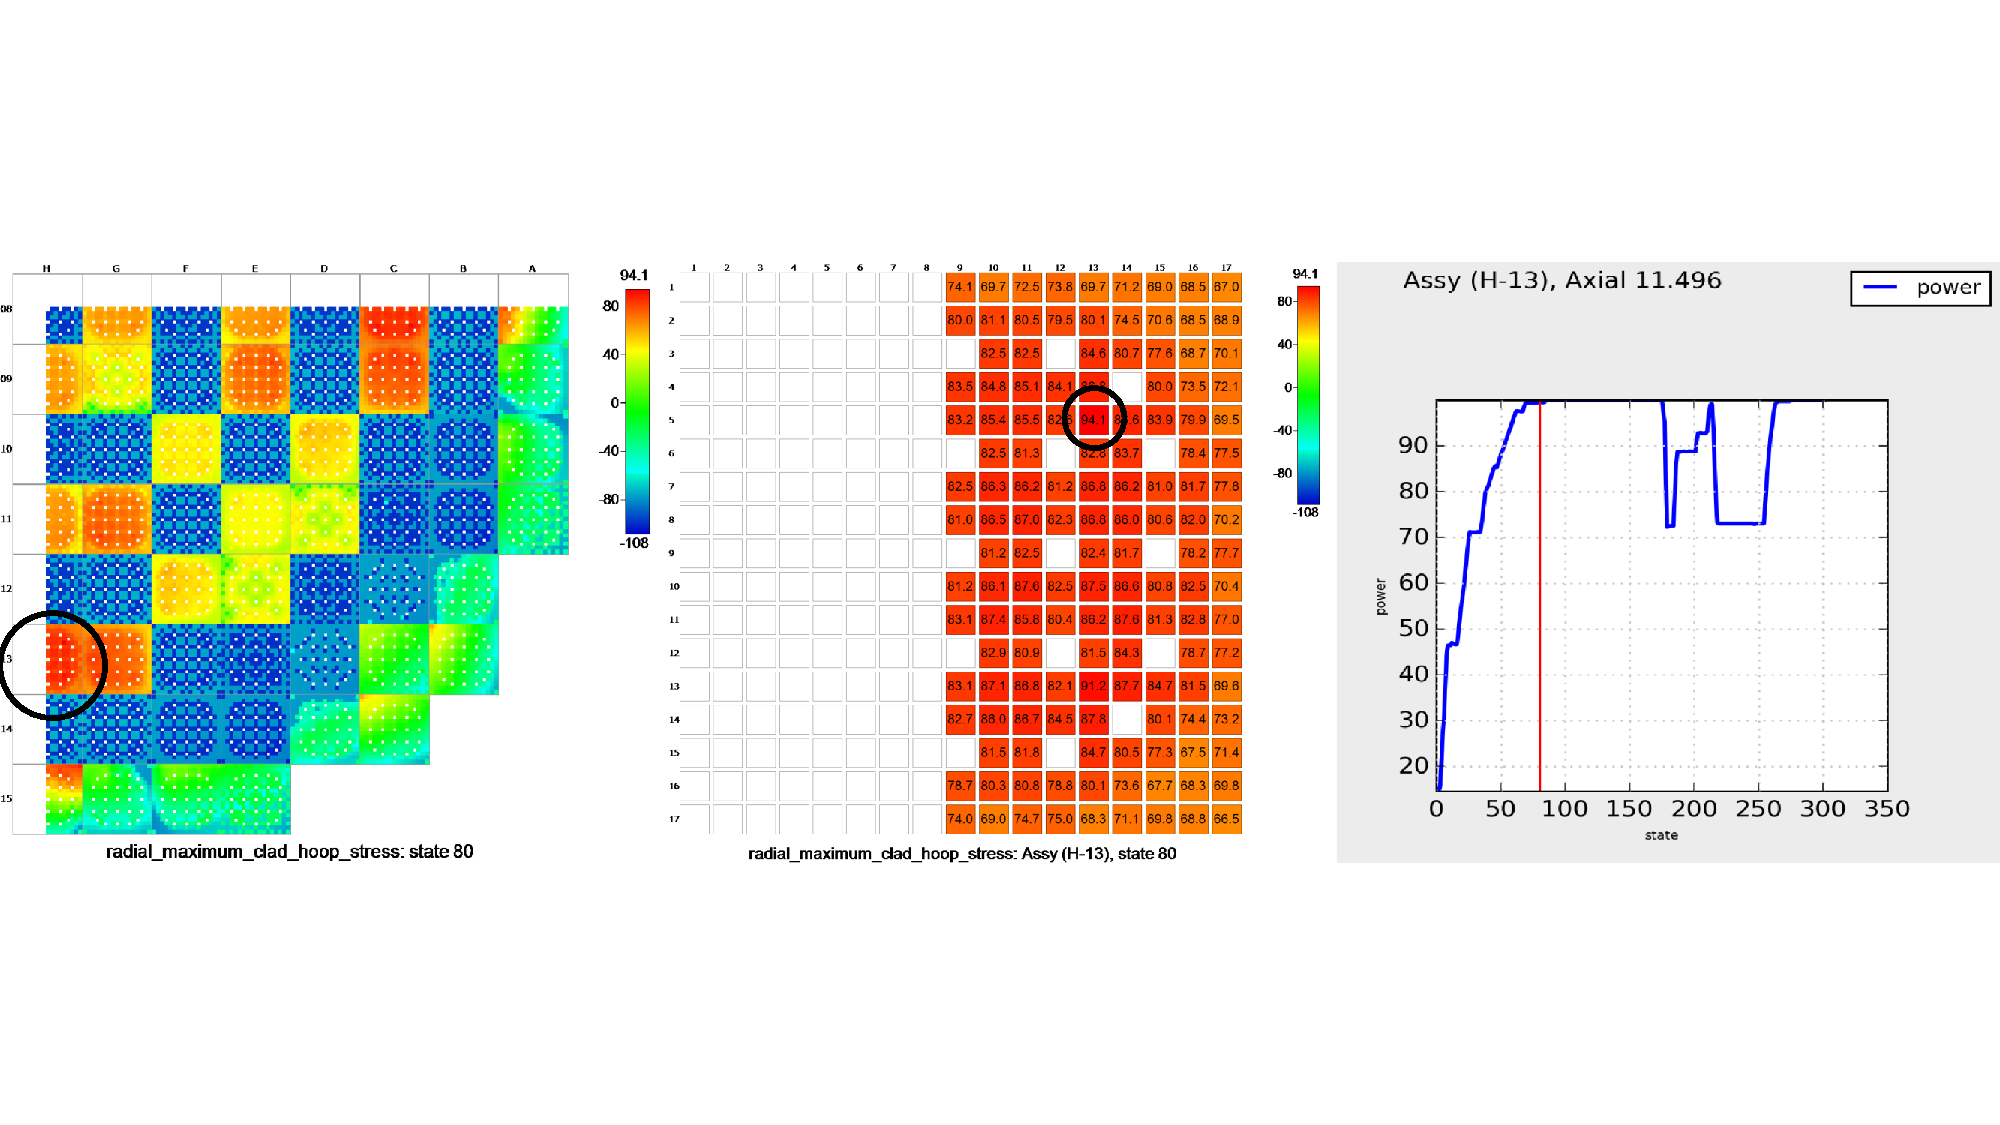
\includegraphics[trim={0 4cm 0 4cm},clip,width=\linewidth]{./Figures/bison_res/IPR_MGD.pdf} \\
\end{tabular}
\caption{BISON predicted maximum clad hoop stress $[MPa]$ (top) and minimum gap distance $[ \mu m]$ (bottom) for start-up power ramp.}
\label{fig:bison_initial}
\end{figure}
\end{landscape}
\begin{landscape}
\begin{figure}[h]
\begin{tabular}{c}
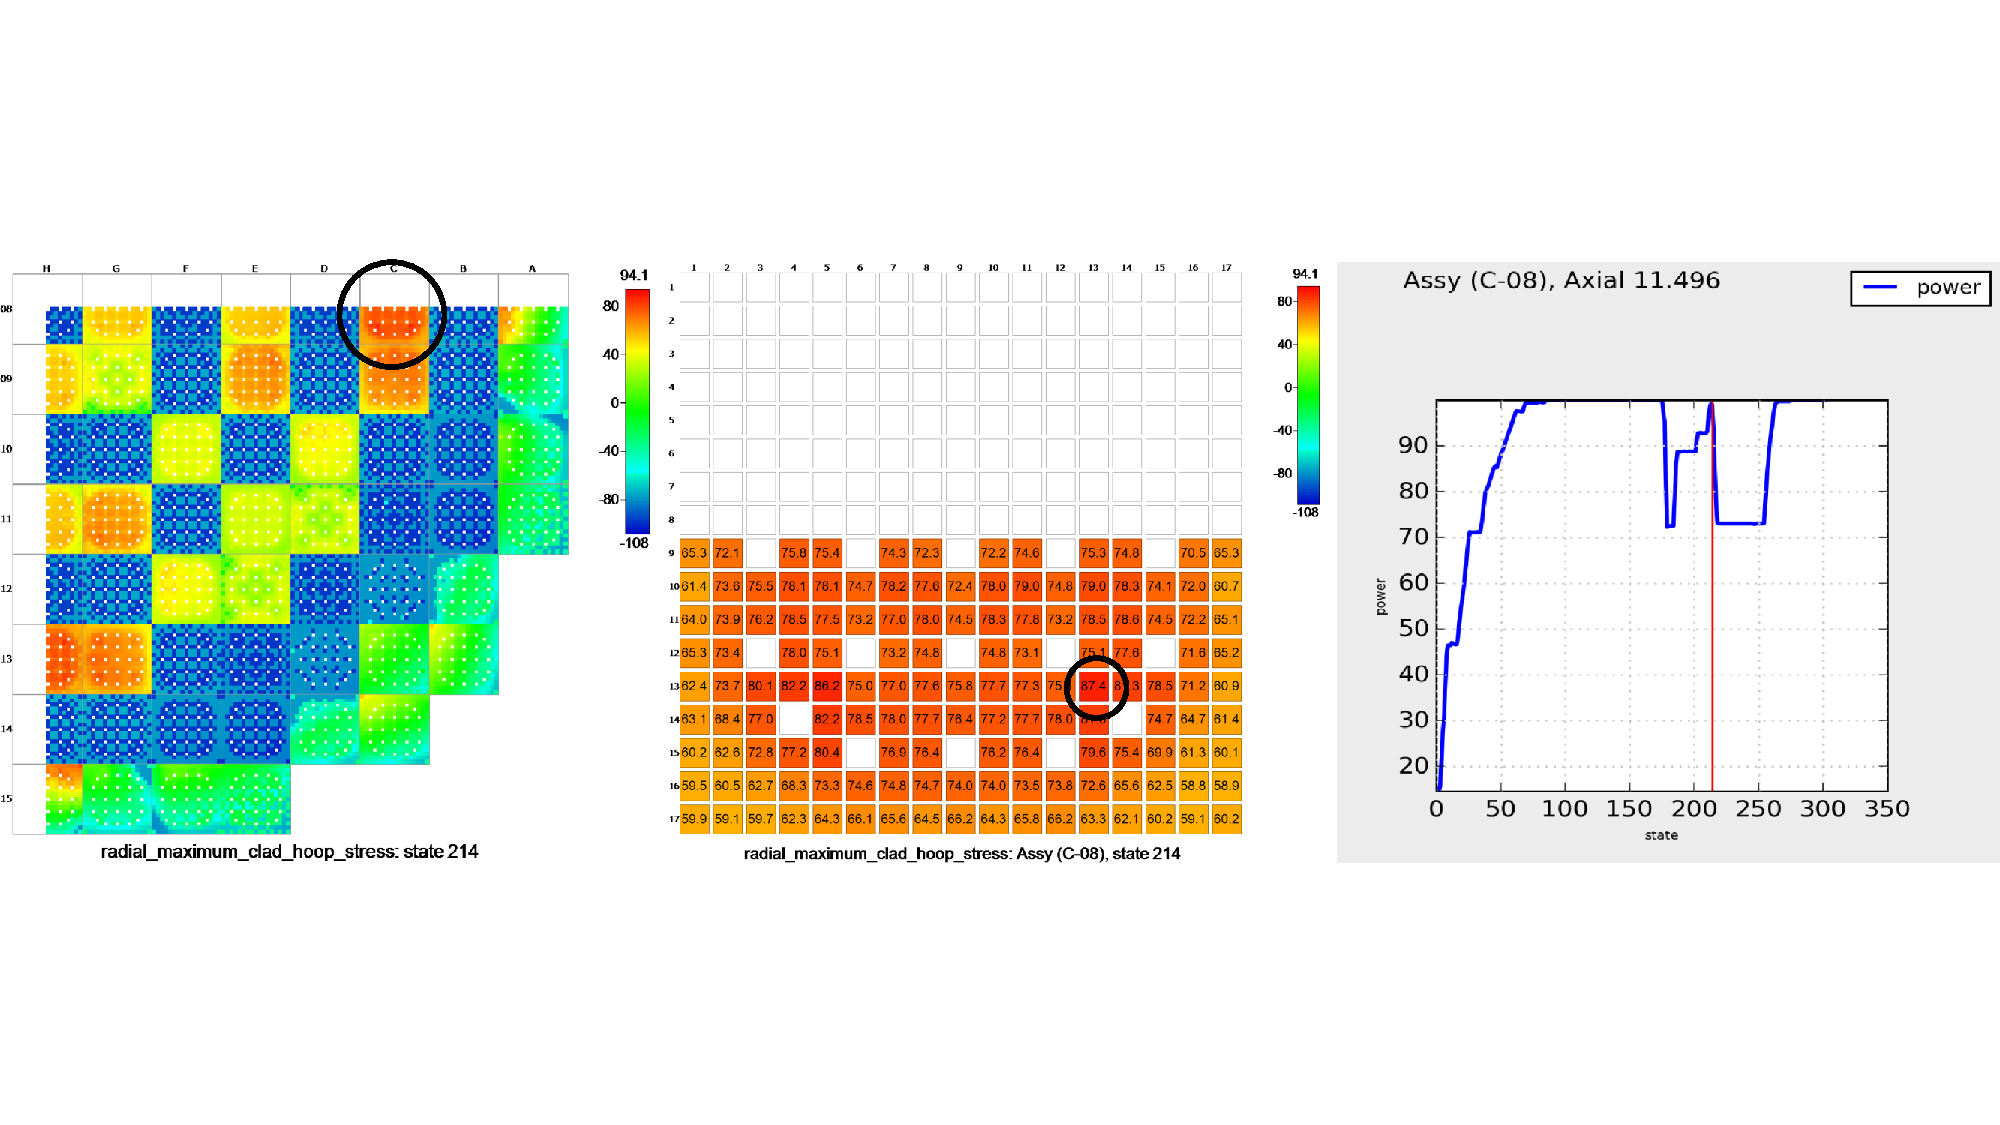
\includegraphics[trim={0 4cm 0 4cm},clip,width=\linewidth]{./Figures/bison_res/PR1_MCHS.pdf} \\
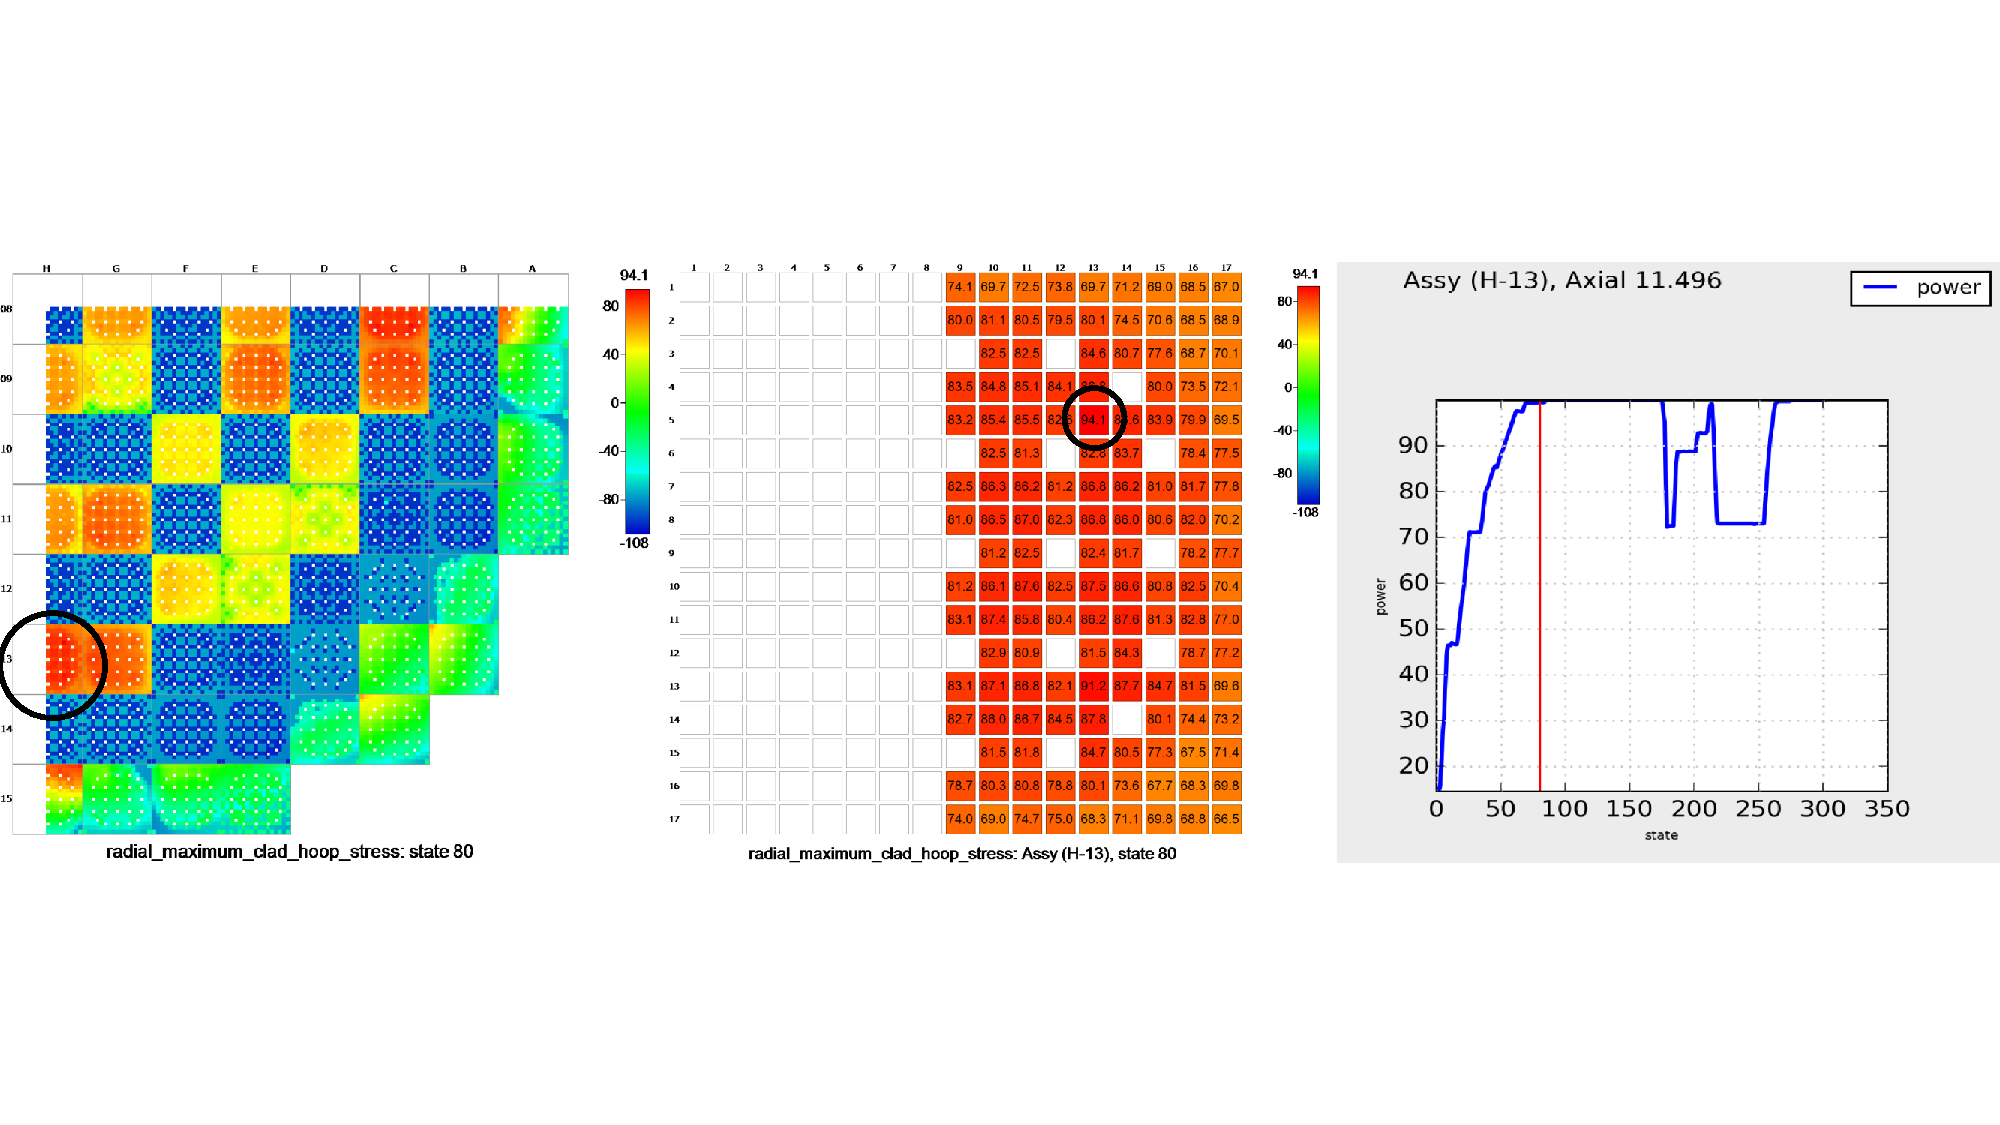
\includegraphics[trim={0 4cm 0 4cm},clip,width=\linewidth]{./Figures/bison_res/PR1_MGD.pdf} \\
\end{tabular}
\caption{BISON predicted maximum clad hoop stress $[MPa]$ (top) and minimum gap distance $[ \mu m]$ (bottom) for the first load-follow power maneuver.}
\label{fig:bison_PR1}
\end{figure}
\end{landscape}

\begin{landscape}
\begin{figure}[h]
\begin{tabular}{c}
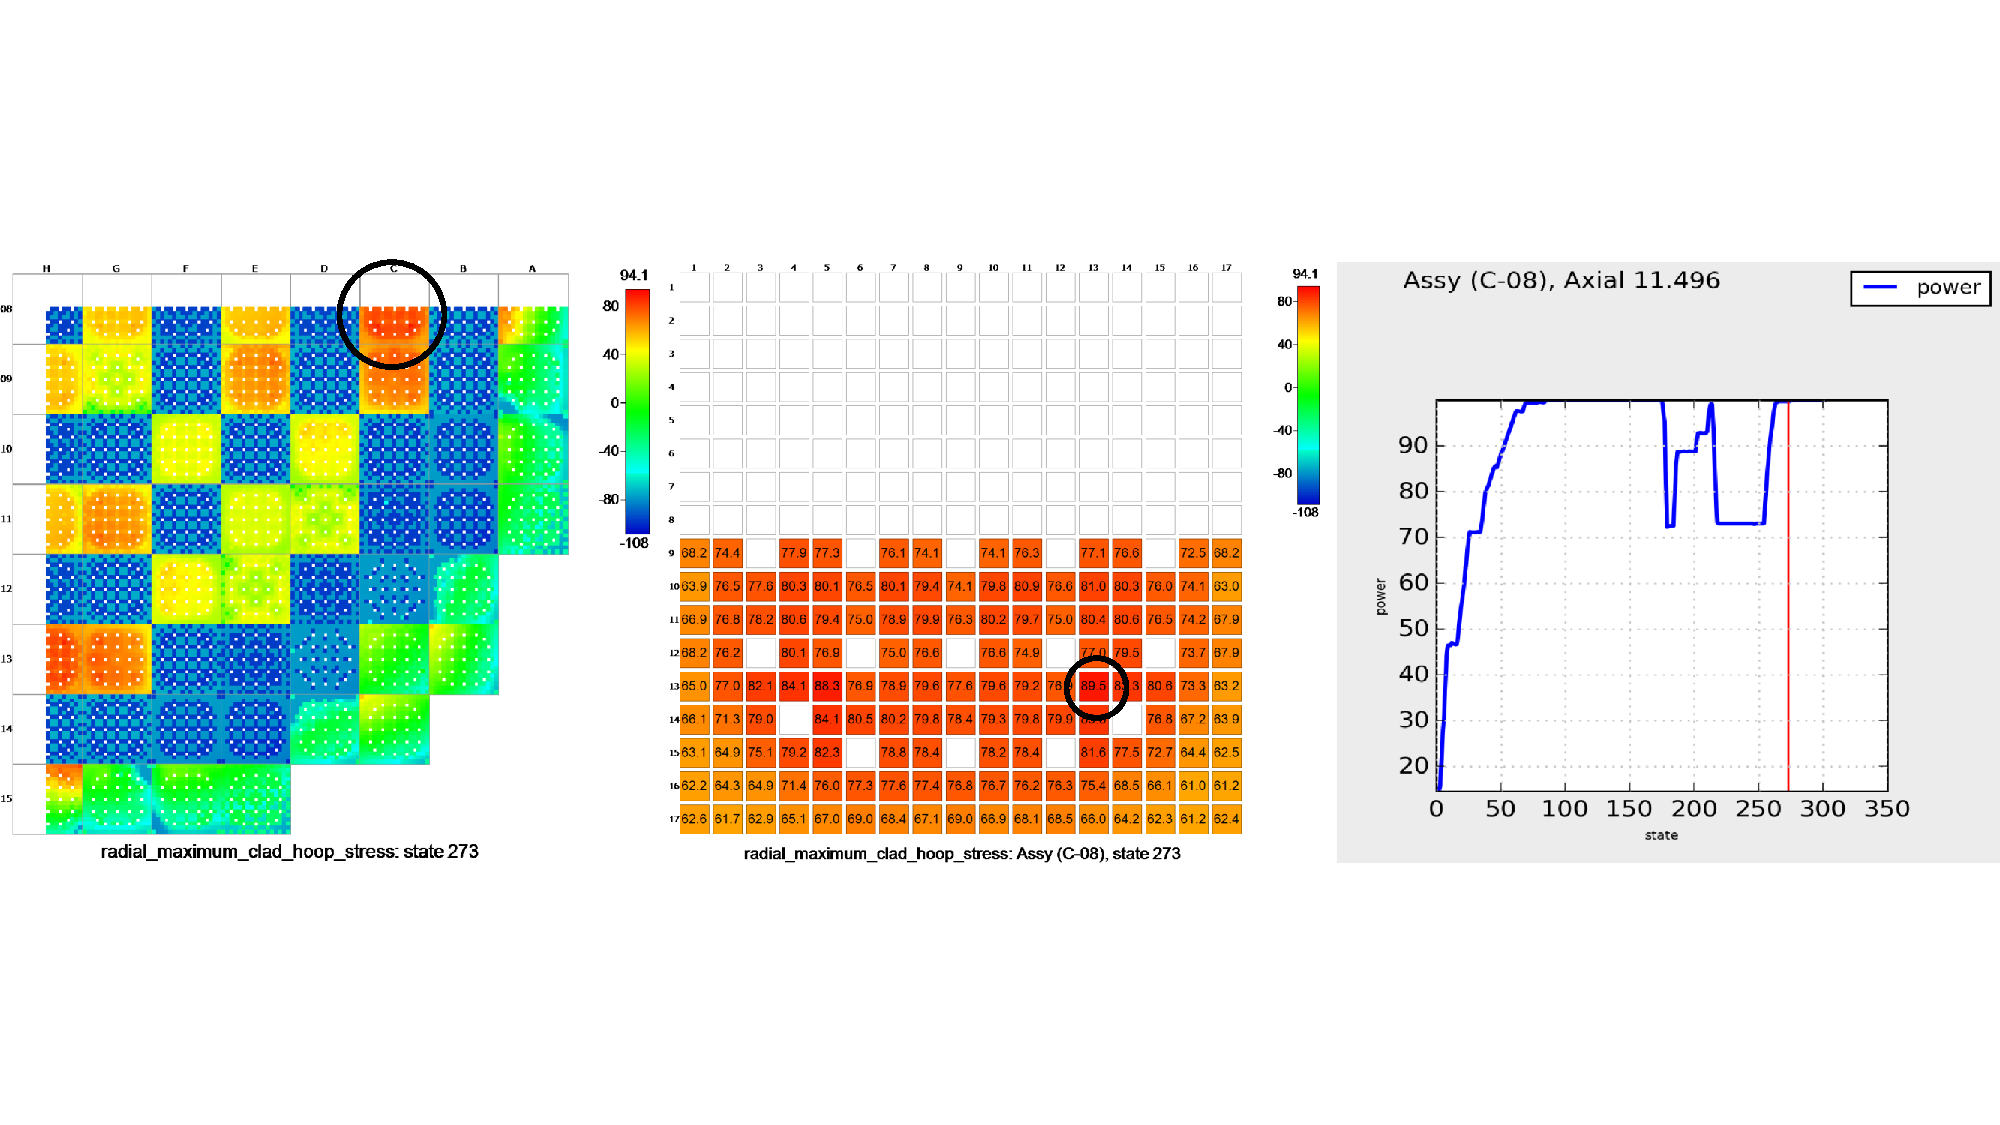
\includegraphics[trim={0 4cm 0 4cm},clip,width=\linewidth]{./Figures/bison_res/PR2_MCHS.pdf} \\
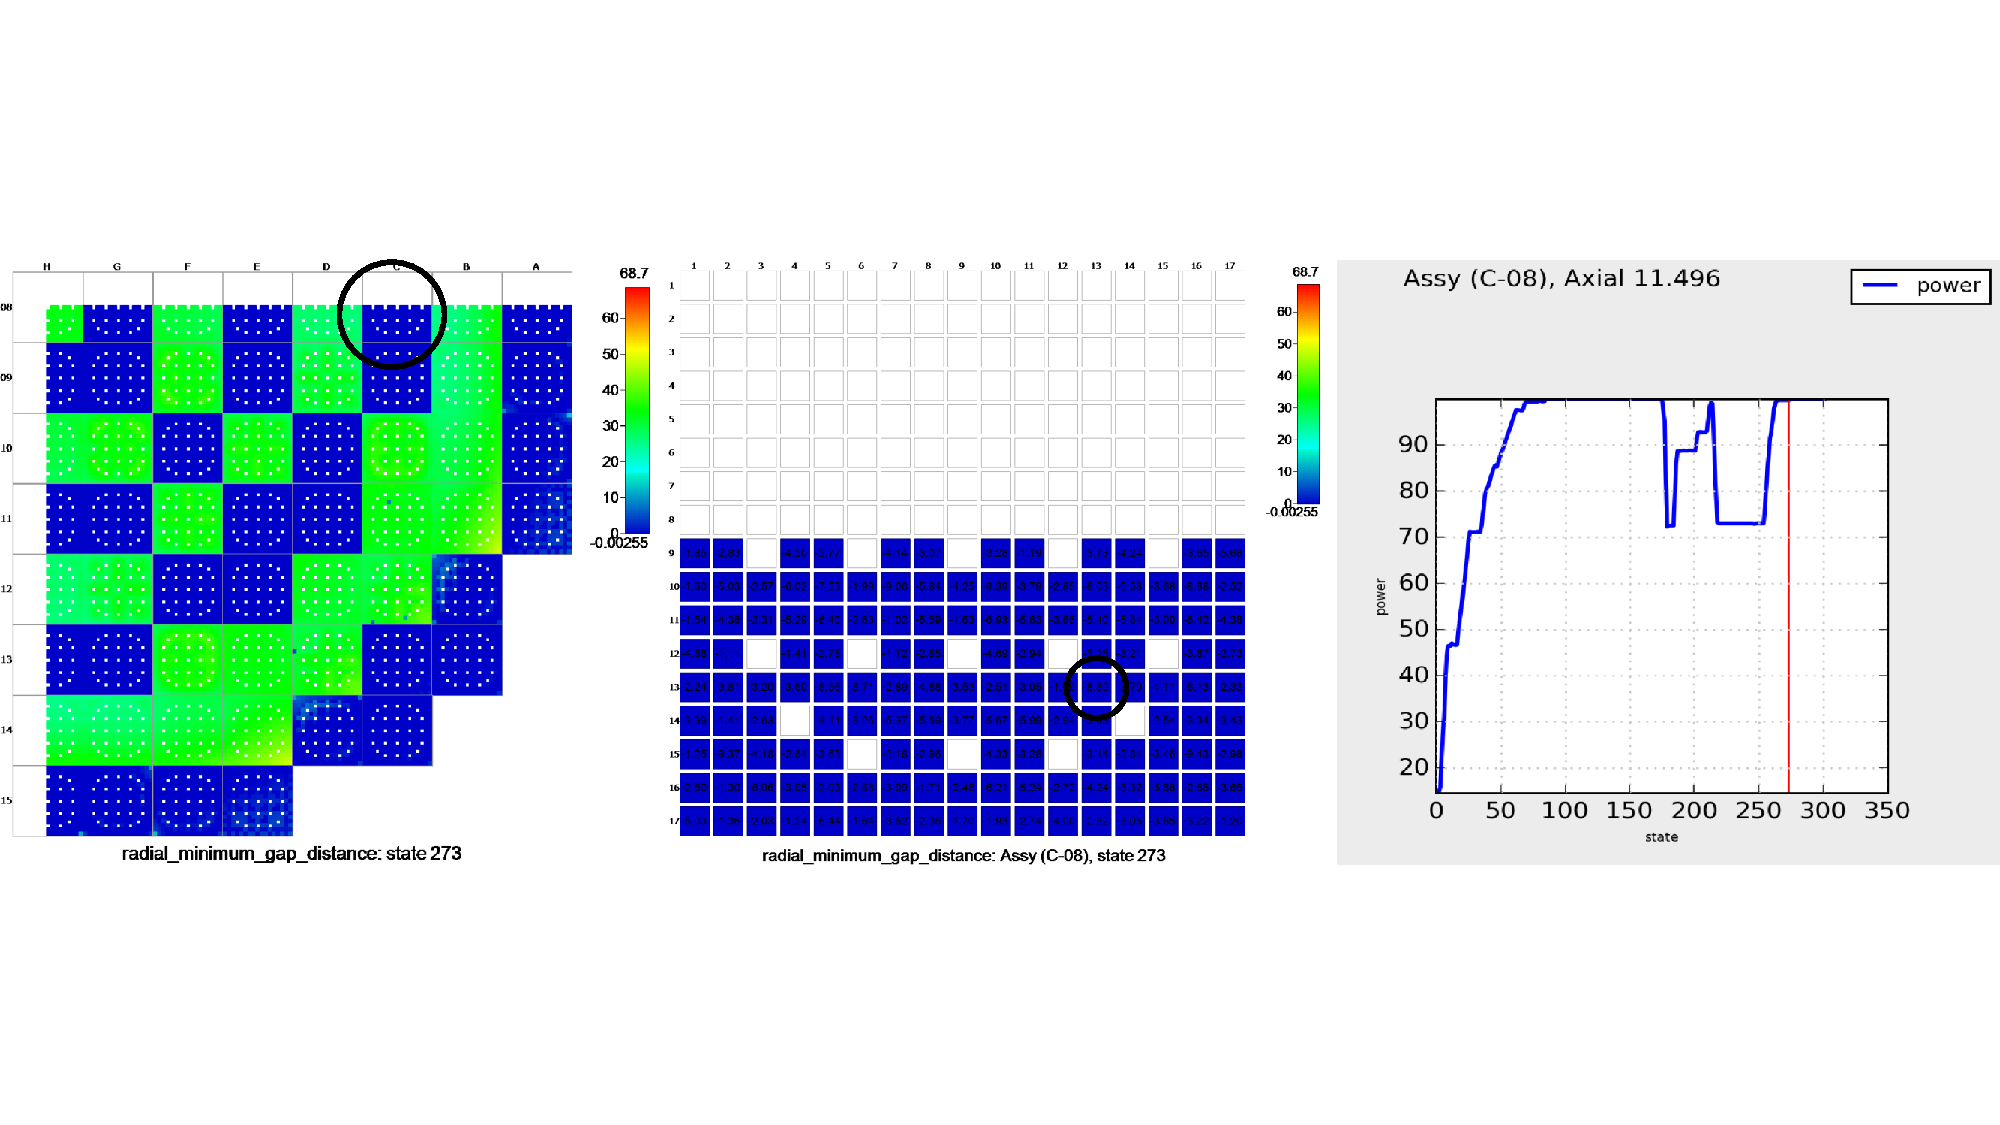
\includegraphics[trim={0 4cm 0 4cm},clip,width=\linewidth]{./Figures/bison_res/PR2_MGD.pdf} \\
\end{tabular}
\caption{BISON predicted maximum clad hoop stress $[MPa]$ (top) and minimum gap distance $[ \mu m]$ (bottom) for the second load-follow power maneuver.}
\label{fig:bison_PR2}
\end{figure}
\end{landscape}

\begin{landscape}
\begin{figure}[h]
\begin{tabular}{c}
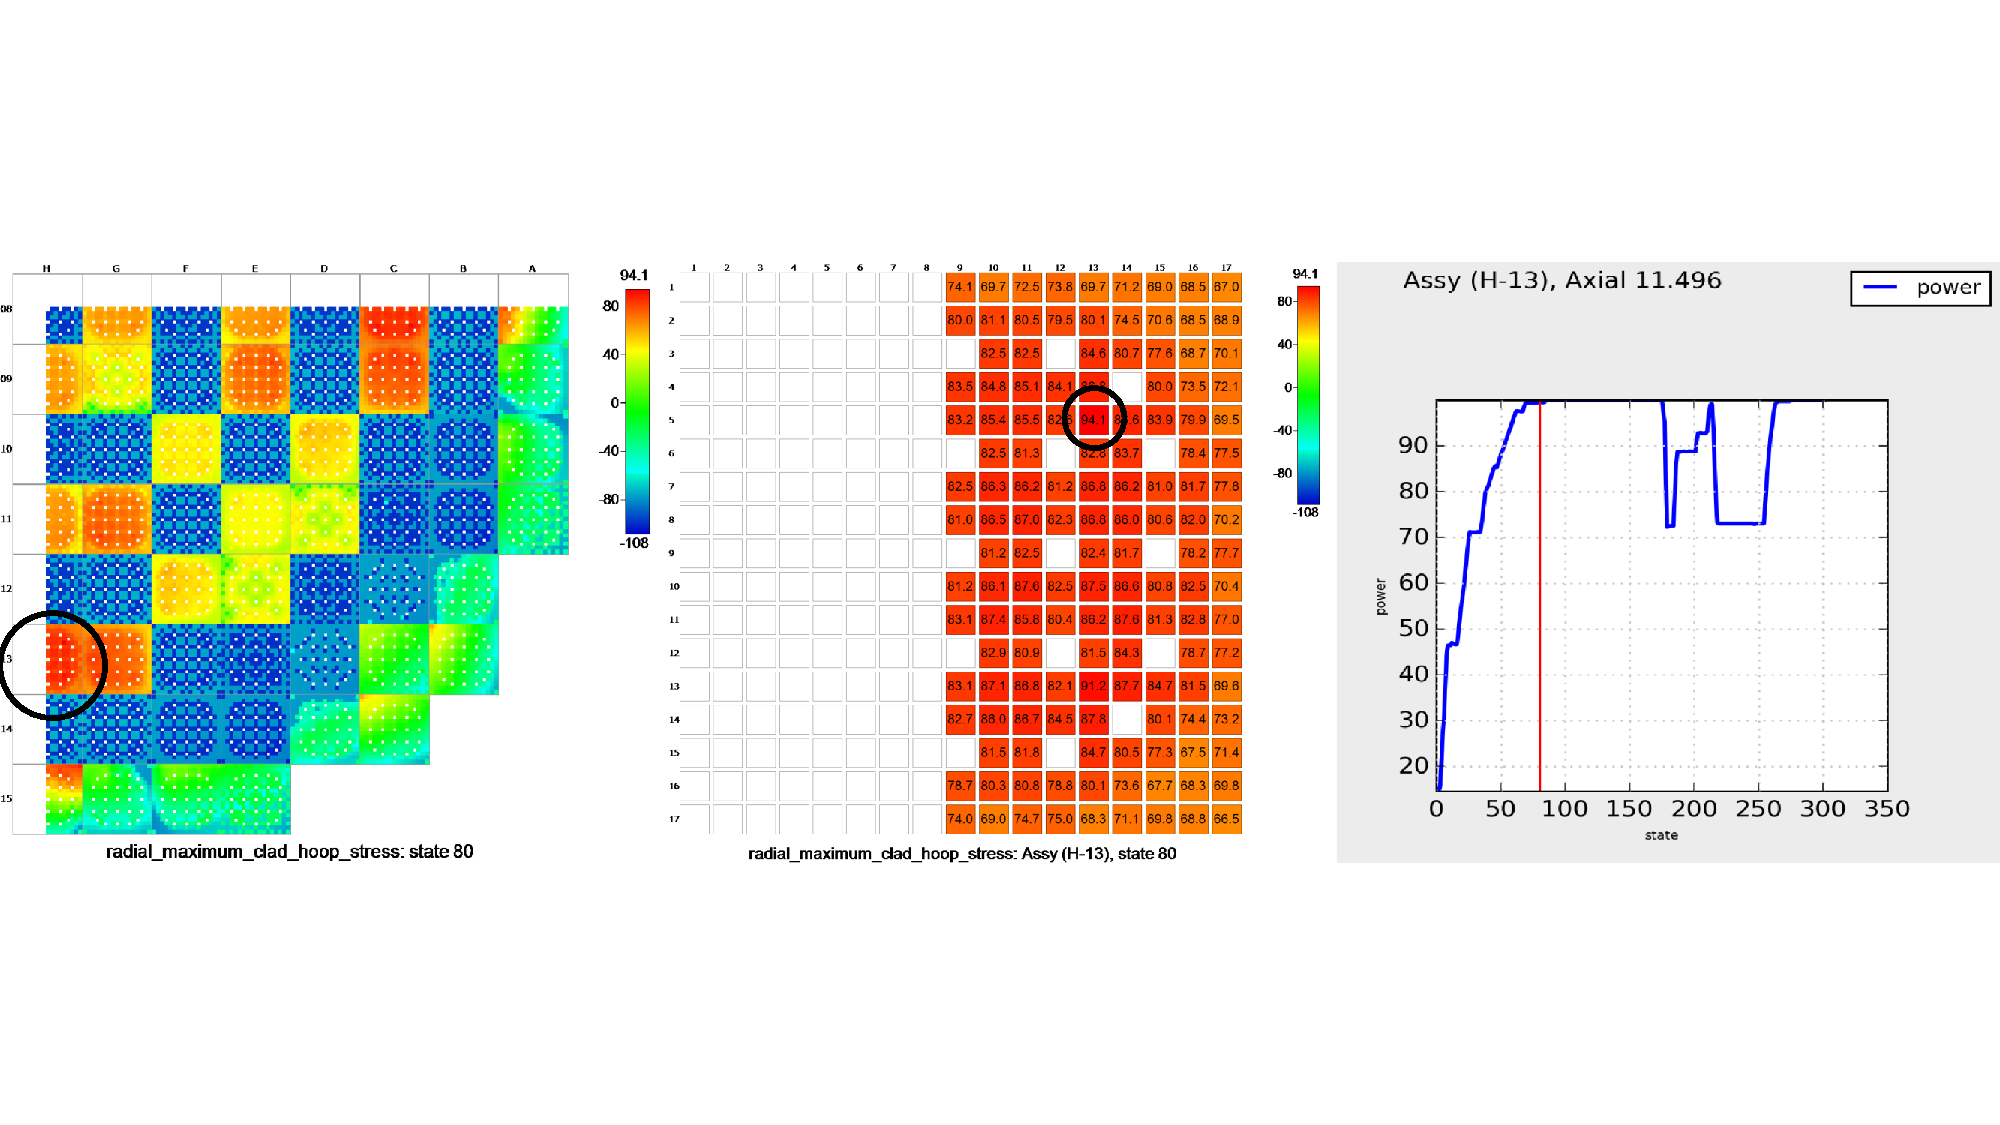
\includegraphics[trim={0 4cm 0 4cm},clip,width=\linewidth]{./Figures/bison_res/PR3_MCHS.pdf} \\
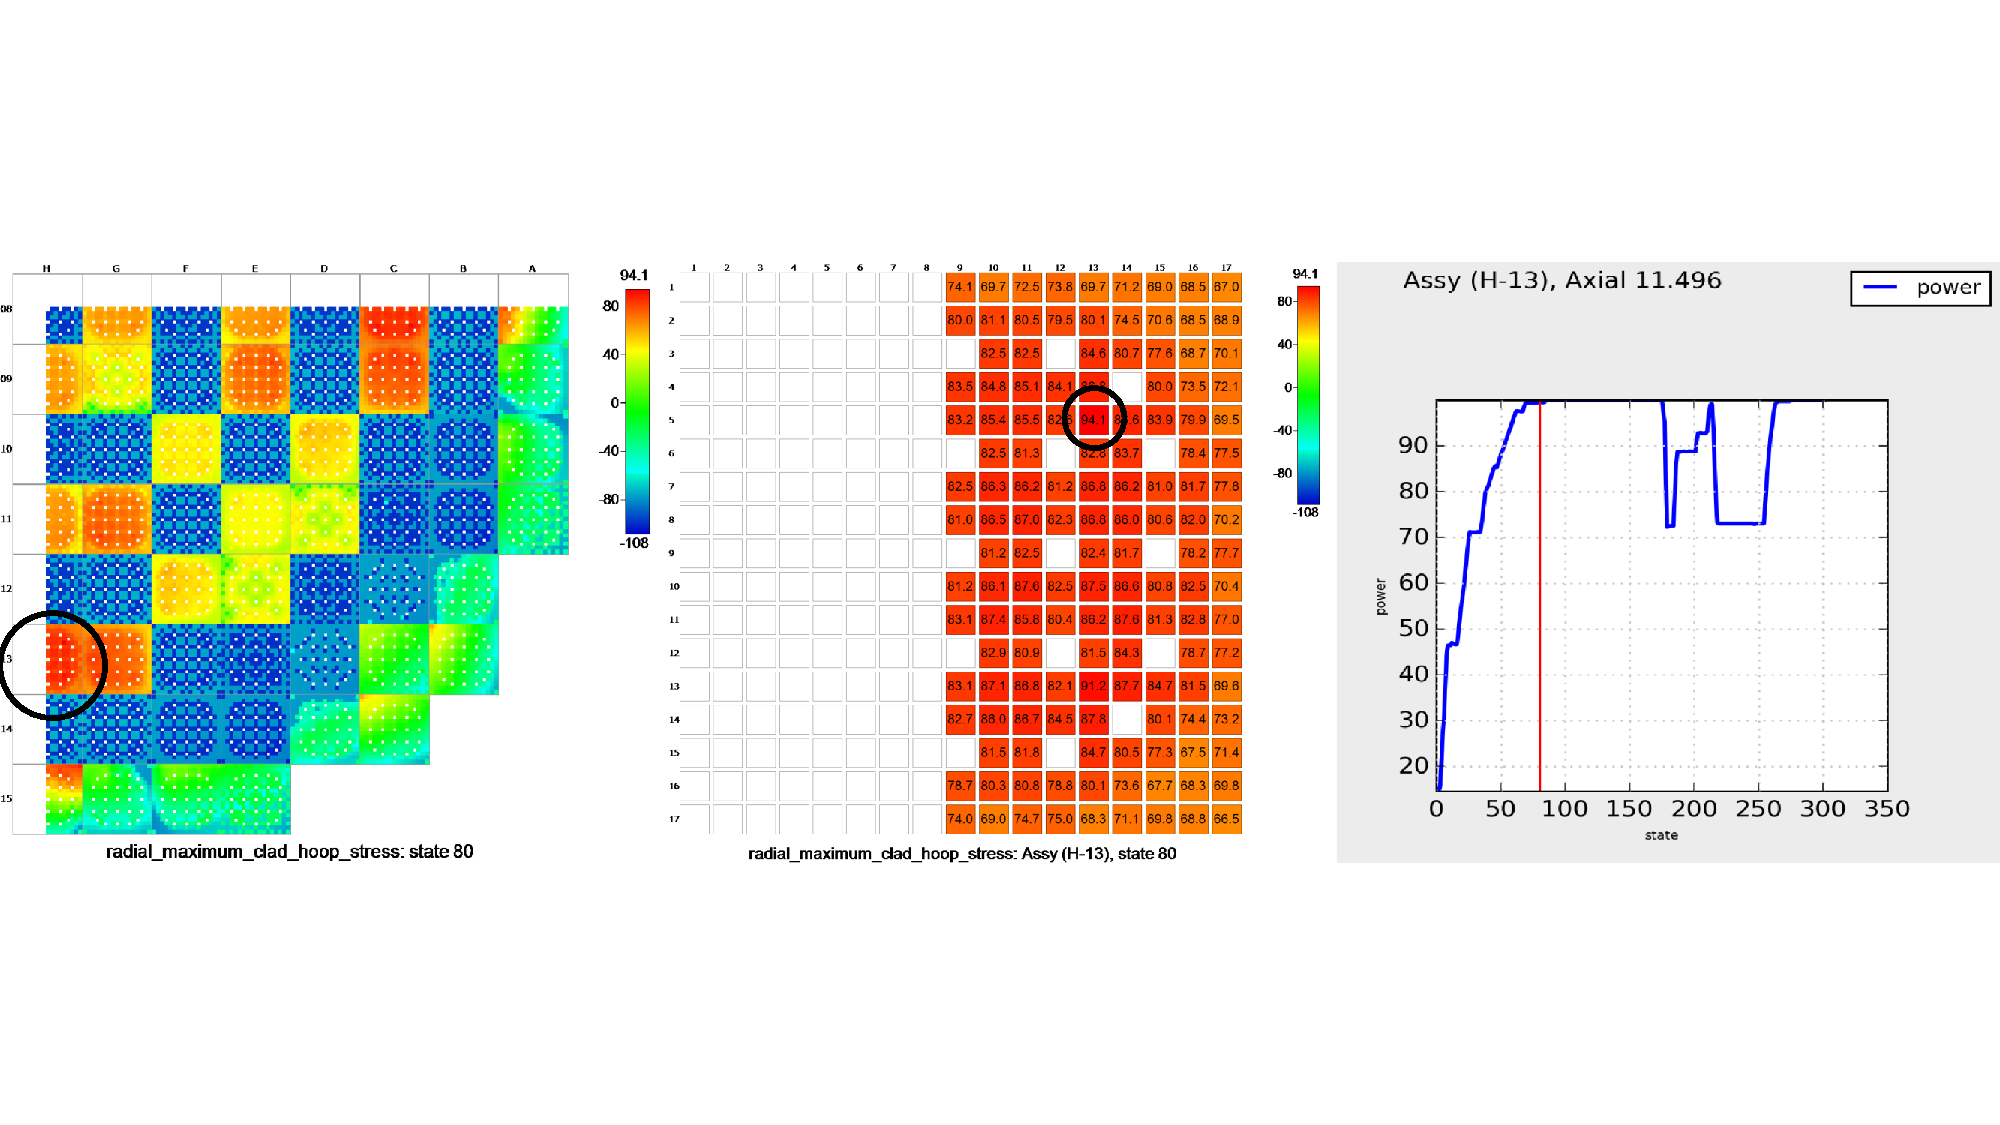
\includegraphics[trim={0 4cm 0 4cm},clip,width=\linewidth]{./Figures/bison_res/PR3_MGD.pdf} \\
\end{tabular}
\caption{BISON predicted maximum clad hoop stress $[MPa]$ (top) and minimum gap distance $[ \mu m]$ (bottom) for the third load-follow power maneuver.}
\label{fig:bison_PR3}
\end{figure}
\end{landscape}

\begin{landscape}
\begin{figure}[h]
\begin{tabular}{c}
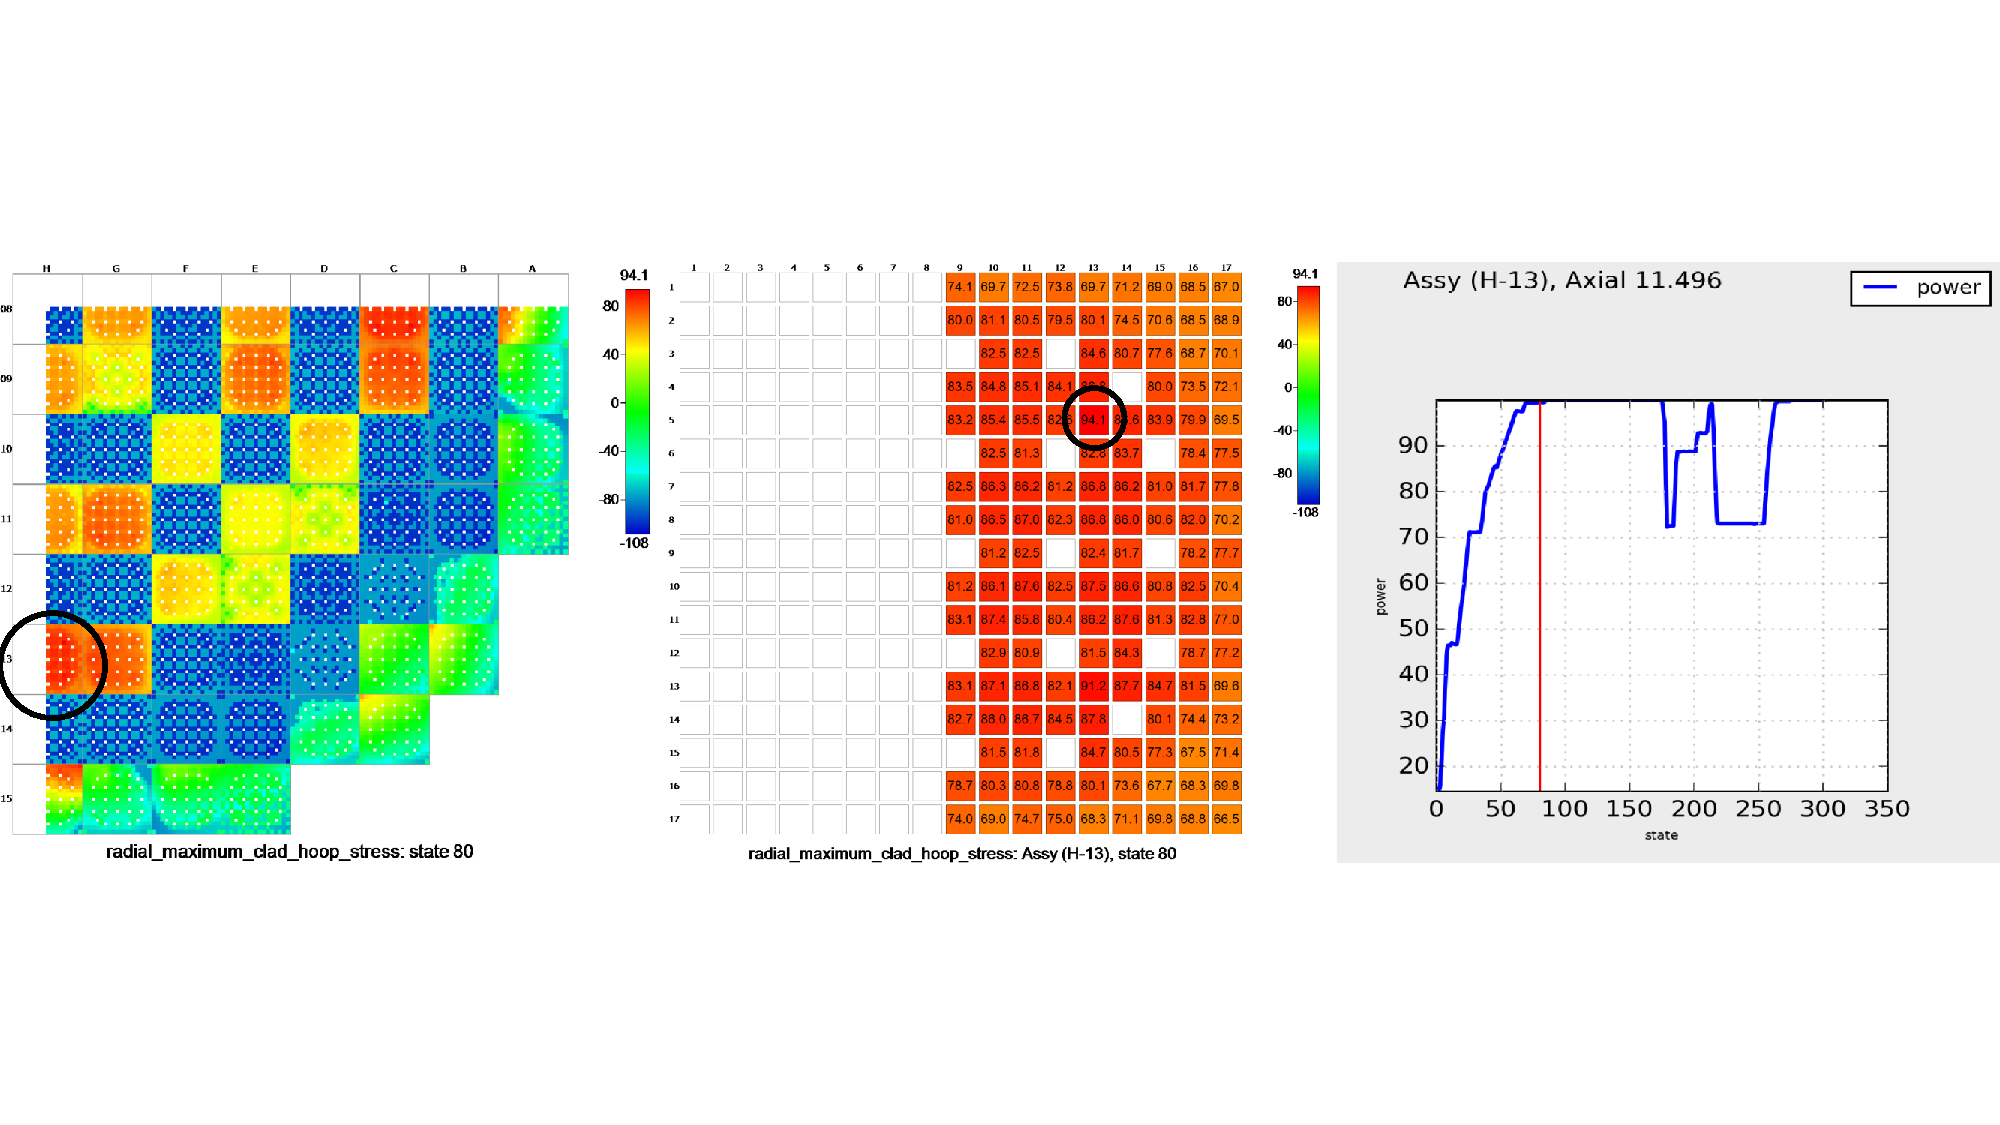
\includegraphics[trim={0 4cm 0 4cm},clip,width=\linewidth]{./Figures/bison_res/PR4_MCHS.pdf} \\
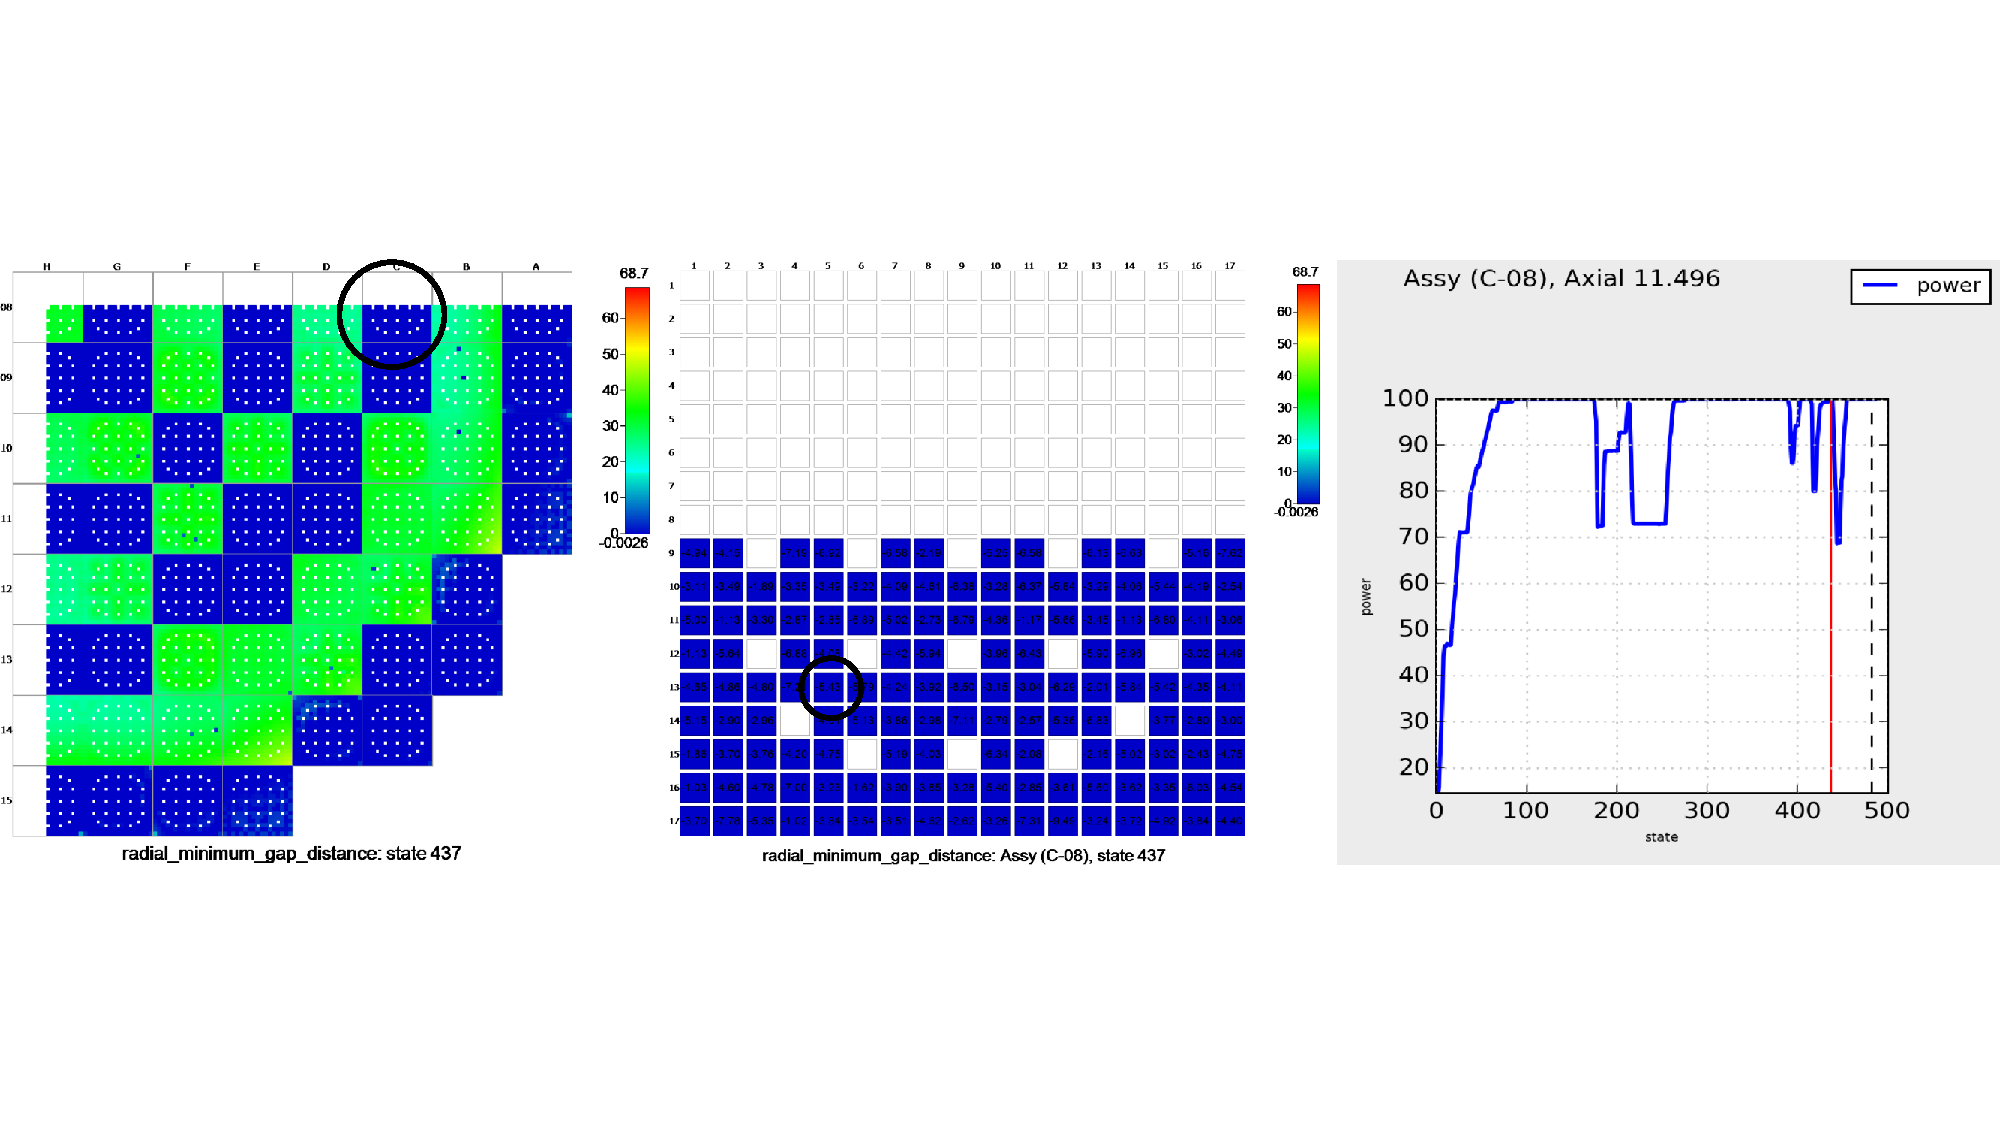
\includegraphics[trim={0 4cm 0 4cm},clip,width=\linewidth]{./Figures/bison_res/PR4_MGD.pdf} \\
\end{tabular}
\caption{BISON predicted maximum clad hoop stress $[MPa]$ (top) and minimum gap distance $[ \mu m]$ (bottom) for the forth load-follow power maneuver.}
\label{fig:bison_PR4}
\end{figure}
\end{landscape}

\begin{landscape}
\begin{figure}[h]
\begin{tabular}{c}
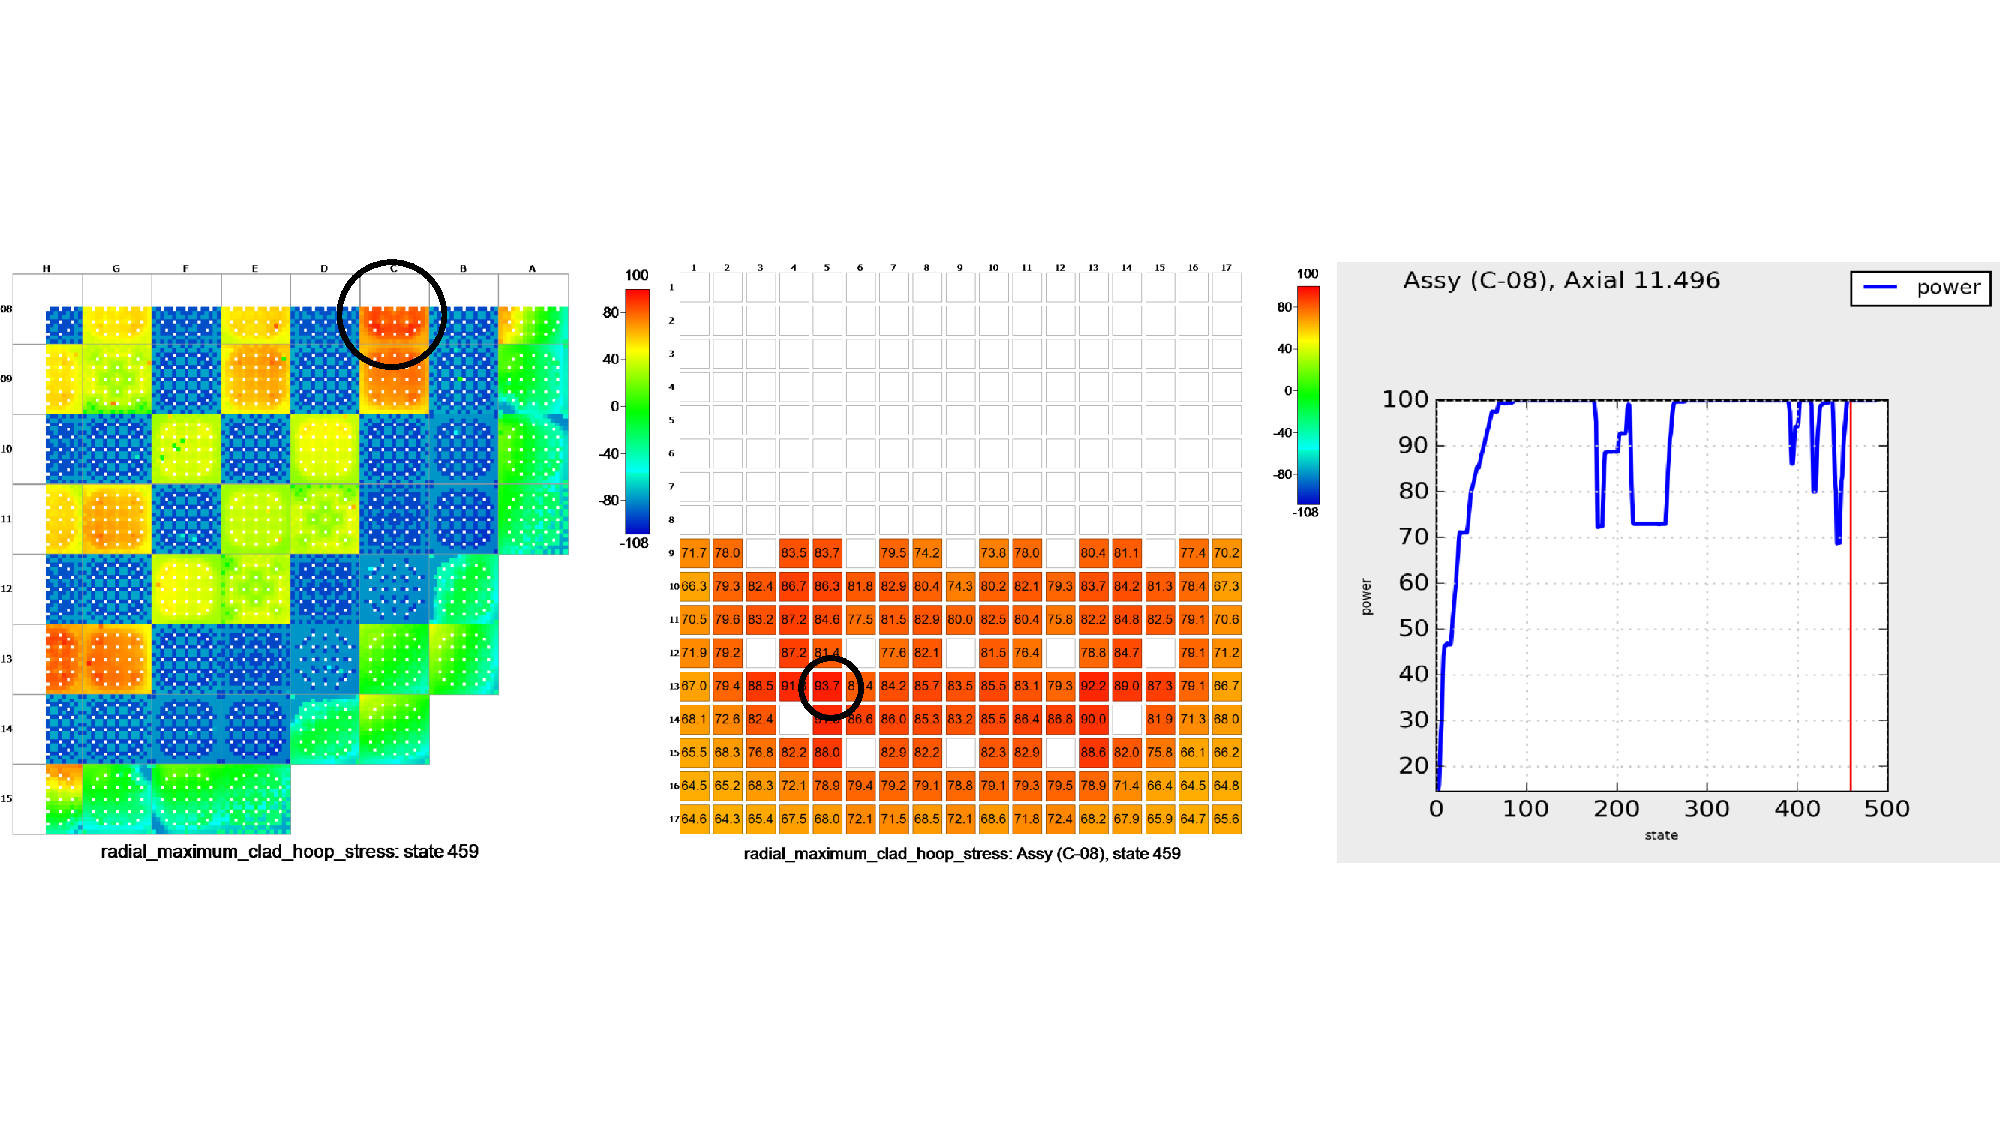
\includegraphics[trim={0 4cm 0 4cm},clip,width=\linewidth]{./Figures/bison_res/PR5_MCHS.pdf} \\
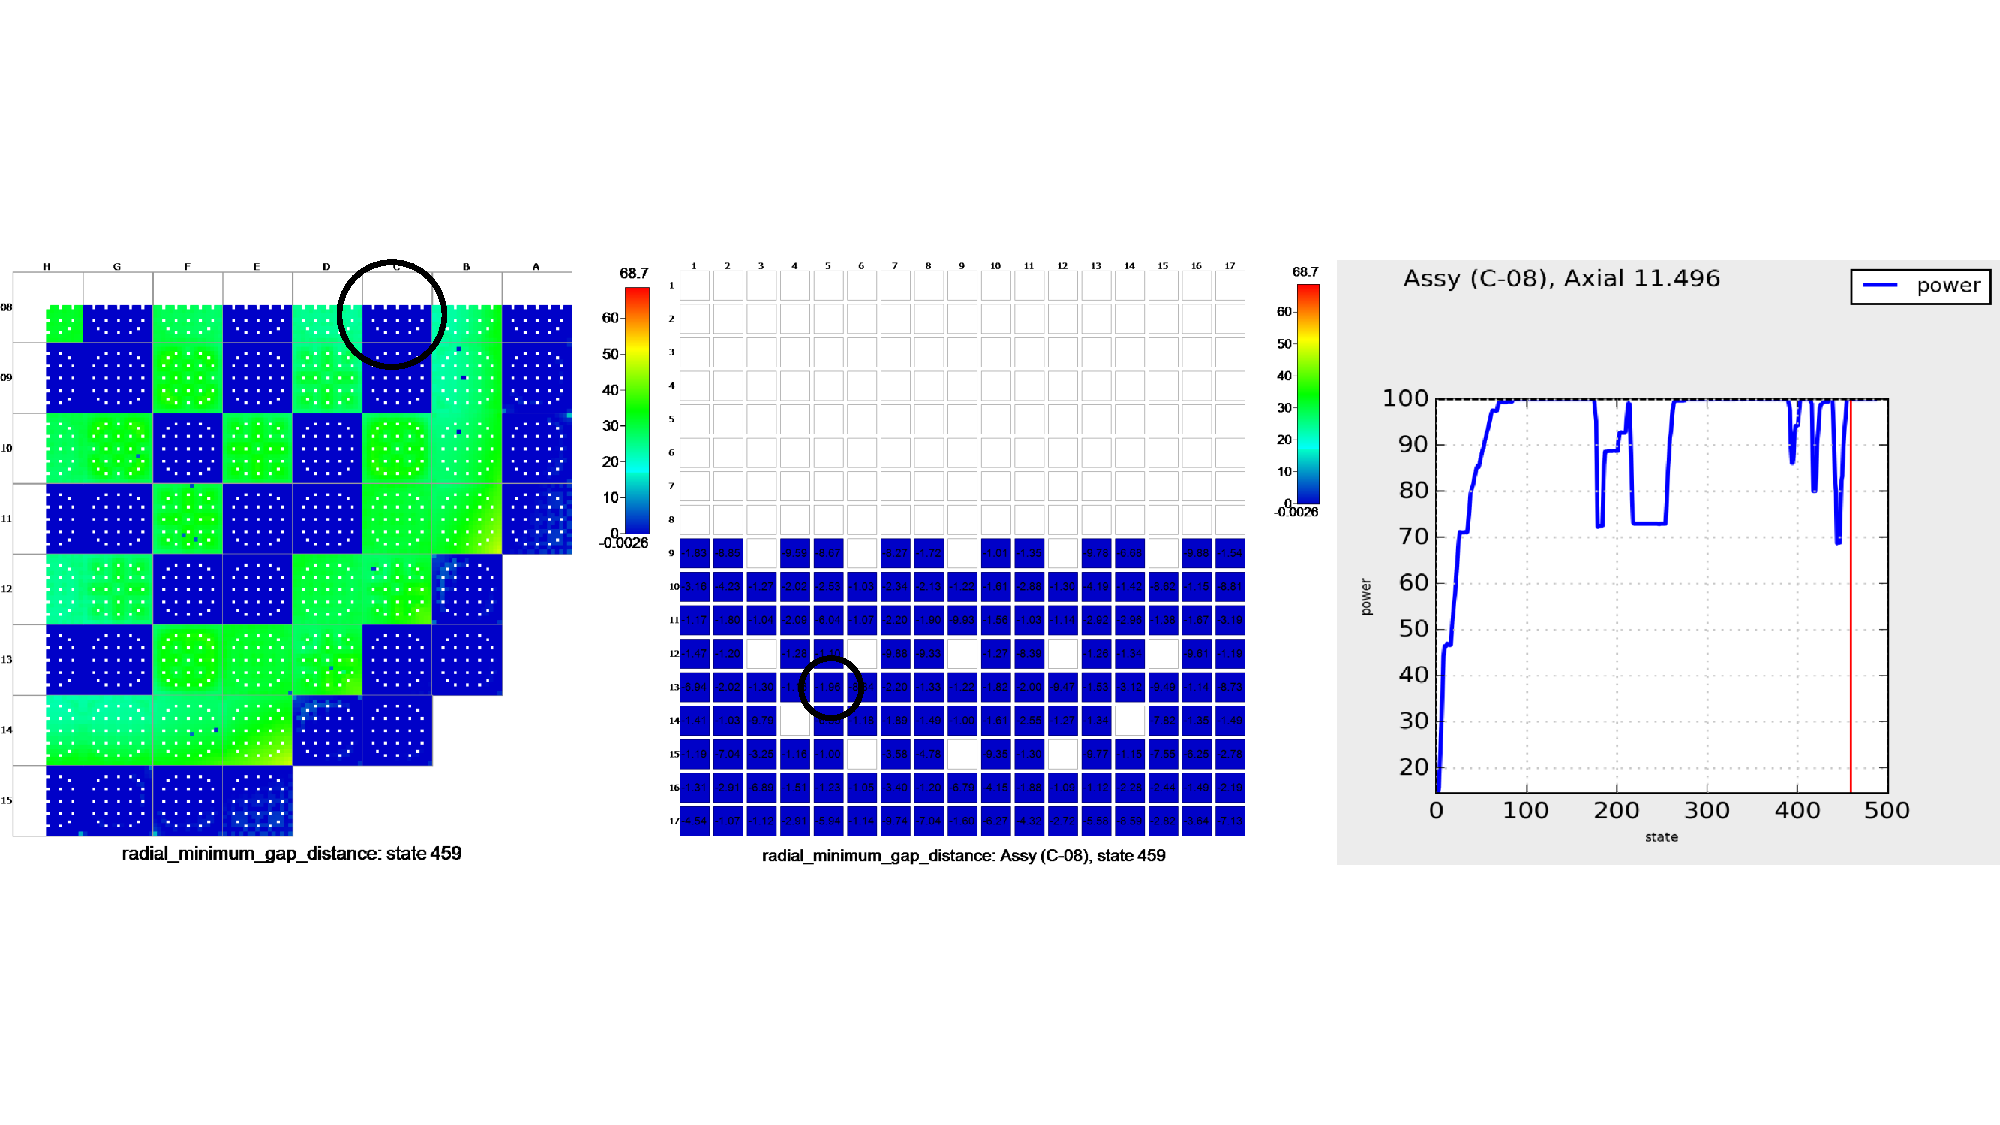
\includegraphics[trim={0 4cm 0 4cm},clip,width=\linewidth]{./Figures/bison_res/PR5_MGD.pdf} \\
\end{tabular}
\caption{BISON predicted maximum clad hoop stress $[MPa]$ (top) and minimum gap distance $[ \mu m]$ (bottom) for the fifth load-follow power maneuver.}
\label{fig:bison_PR5}
\end{figure}
\end{landscape}


%%%%%%%%%%%%%%%%%%%%%%%%%%%%%%%%%%%%%%%%%%%%%%%%%%%%%%%%%
\section{Limiting Pin}
%%%%%%%%%%%%%%%%%%%%%%%%%%%%%%%%%%%%%%%%%%%%%%%%%%%%%%%%%

The weighted change in linear heat rate determined using the MPACT load-follow results are presented in Figures \ref{fig:lf_PR1} -- \ref{fig:lf_PR3}.
In each figure, negative changes are masked in order to highlight the fuel rods of interest.
%Although the weighted change is a product of burnup, which is constantly increasing, and linear heat rate,
Local maxima were observed six to eight hours after a return to full power.
Each maxima corresponds to the time when a local maximum was observed in the cladding max hoop stress.
Unfortunately the fuel pin with the maximum weighted change in linear heat rate did not exhibit the maximum cladding hoop stress. 
Nonetheless, 1000 fuel pins were selected from the quarter core results based on their weighted change in linear heat rates.
For all simulated power ramps, the fuel pin containing the maximum clad hoop stress was contained within the selected group.
 
A comparison between the 1000 fuel pins with the highest maximum clad hoop stress and the 1000 fuel pins with the highest weighted change in linear heat rate is presented in Figures \ref{fig:comp}.
The figure contains five radial core maps where a blue square represents a pin that was only identified by its change in linear heat rate, a green square represents a pin that was only identified by its clad hoop stress and a red square was identified by both its change in linear heat rate and its clad hoop stress.
Although the weighted change in linear heat rate is able to capture the maximum hoop stress, its main objective, the comparison of the extrema highlights potential problems with this screening method.
In the second core map several pins from two assemblies are only identified by the linear heat rate.
These pins, which are in close proximity of the fresh fuel assemblies, are only experiencing hoop stresses in the range 40 MPa, less then half the maximum value.
This suggests that the weighting by linear heat rate introduces a dependence on position.
Fuel pins in close proximity to fresh fuel are likely to be selected by the screening process even though their change from conditioned power may be minimal.
This effect is also observed in the other four core maps, as many of the pins only identified by the screening process are adjacent to fresh fuel.
As the cycle continues the radial power distribution will flatten reducing the importance of the linear heat weighting.

Another negative consequence of the linear heat rate weighting is that two inner assemblies had no fuel pins identified during the screening process.
These fuel pins, shown in green, are present in all 5 core maps and have hoop stresses in close proximity of the maximum.
In the later power ramps, ramps 3 and 4, some of the fuel pins within these assemblies were identified by the screening process.
Additional accuracy will be required before a complete transition to a pin based screening process can take place.
Nonetheless, the objective of the screening process, contain the maximum cladding hoop stress, was achieved and the majority of the fuel pins identified by the process did show elevated cladding hoop stresses.

\begin{landscape}
\begin{figure}[h]
\begin{tabular}{c}
\includegraphics[trim={0 4cm 0 4cm},clip,width=\linewidth]{./Figures/screening/PR1.pdf} \\
\includegraphics[trim={0 4cm 0 4cm},clip,width=\linewidth]{./Figures/screening/PR2.pdf} \\
\end{tabular}
\caption{Weighted change in linear heat rate for the first (top) and second (bottom) load-follow power maneuver.}
\label{fig:lf_PR1}
\end{figure}
\end{landscape}

\begin{landscape}
\begin{figure}[h]
\begin{tabular}{c}
\includegraphics[trim={0 4cm 0 4cm},clip,width=\linewidth]{./Figures/screening/PR3.pdf} \\
\includegraphics[trim={0 4cm 0 4cm},clip,width=\linewidth]{./Figures/screening/PR4.pdf} \\
\end{tabular}
\caption{Weighted change in linear heat rate for the third (top) and forth (bottom) load-follow power maneuver.}
\label{fig:lf_PR2}
\end{figure}
\end{landscape}

\begin{landscape}
\begin{figure}[h]
\begin{tabular}{c}
\includegraphics[trim={0 4cm 0 4cm},clip,width=\linewidth]{./Figures/screening/PR5.pdf} \\
\includegraphics[trim={0 4cm 0 4cm},clip,width=\linewidth]{./Figures/screening/PR5.pdf} \\
\end{tabular}
\caption{Weighted change in linear heat rate for the fifth (top) and forth (bottom) load-follow power maneuver.}
\label{fig:lf_PR3}
\end{figure}
\end{landscape}

\begin{center}
\begin{figure}[h]
\begin{tabular}{lr}
\multicolumn{2}{c}{Blue -- Screening process predicted limiting pin, Green -- BISON predicted limiting pin, Red -- Screening process and BISON predicted limiting pin,} \\
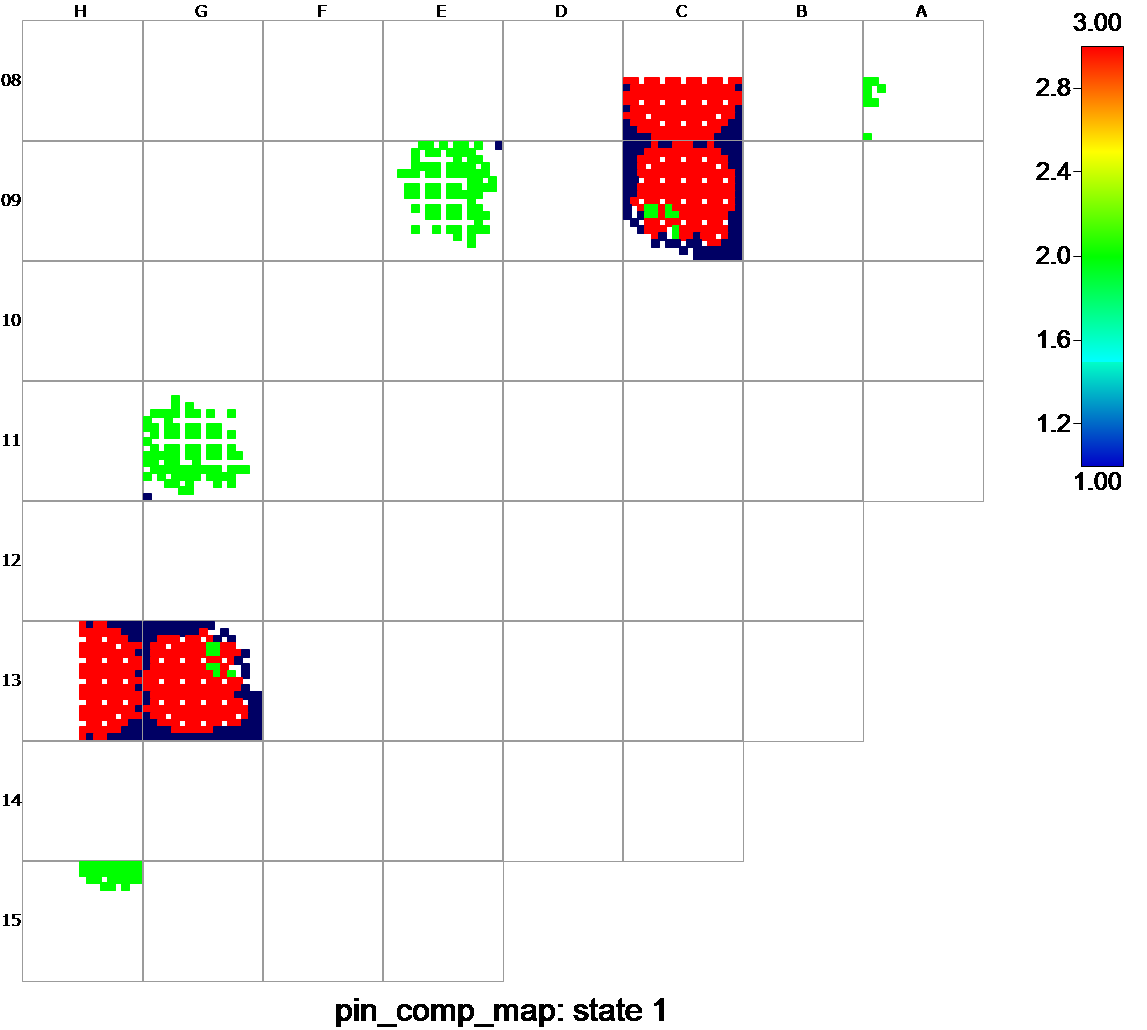
\includegraphics[trim={0 0 4.5cm 0},clip,width=0.4\linewidth]{./Figures/screening/comp1.png} & 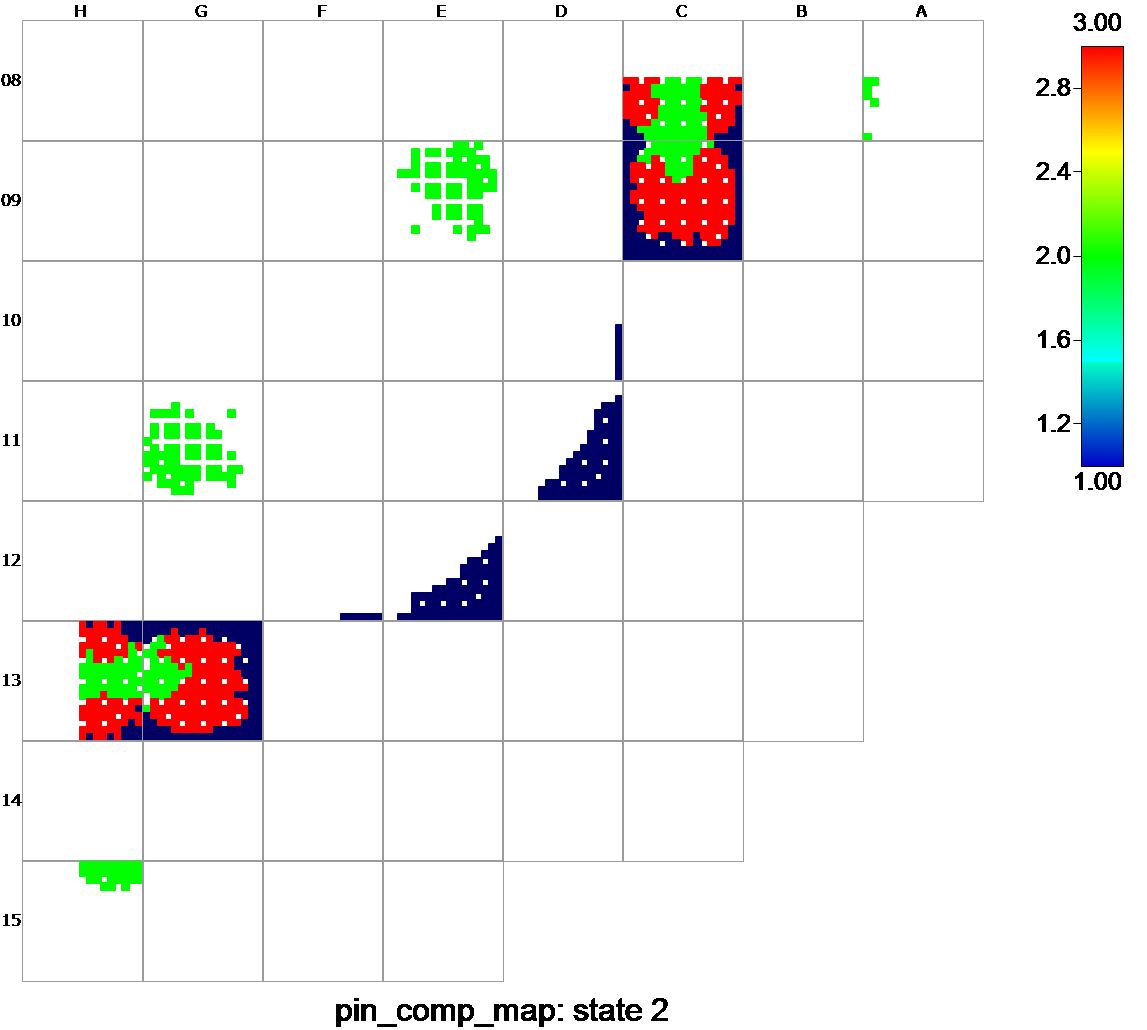
\includegraphics[trim={0 0 4.5cm 0},clip,width=0.4\linewidth]{./Figures/screening/comp2.png} \\
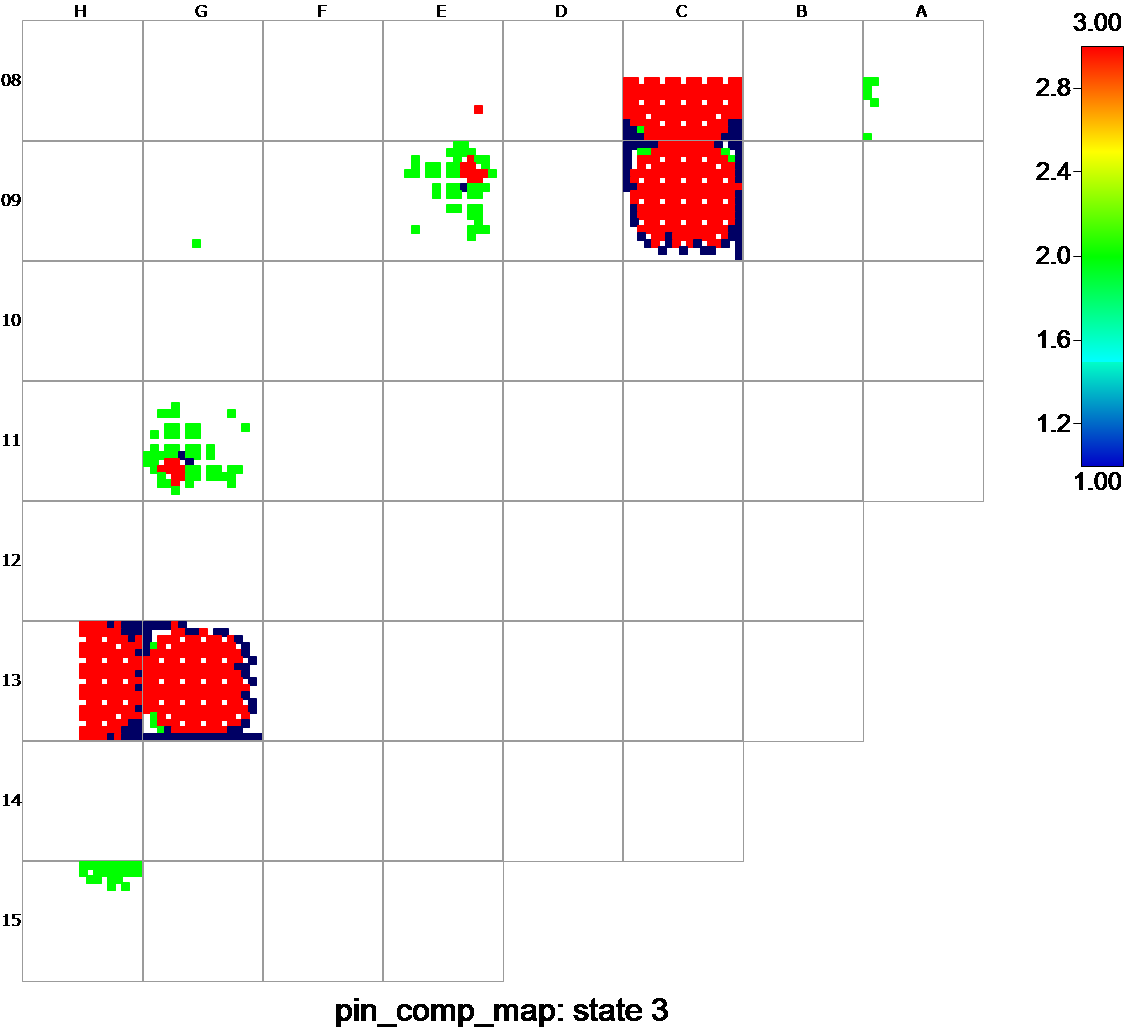
\includegraphics[trim={0 0 4.5cm 0},clip,width=0.4\linewidth]{./Figures/screening/comp3.png} & 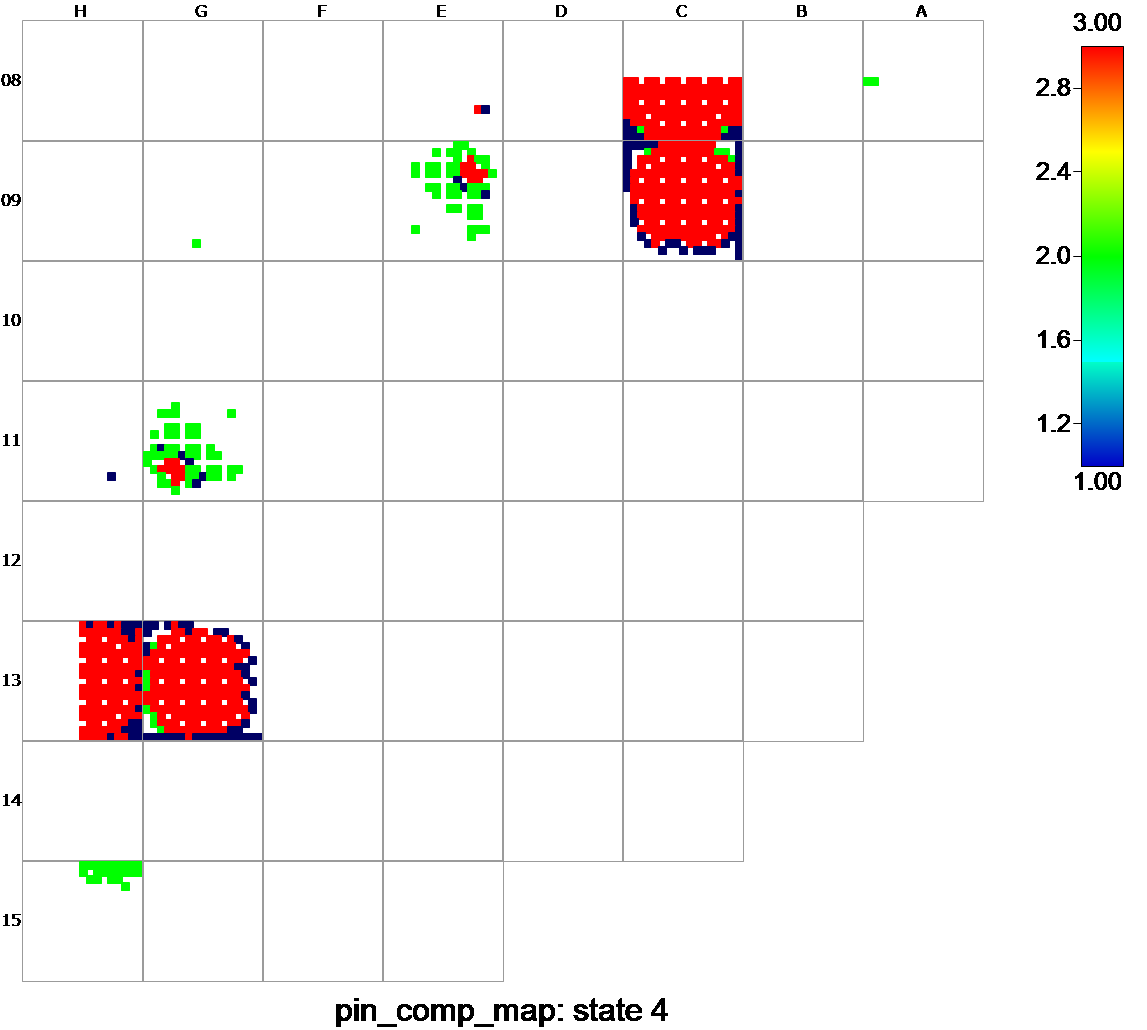
\includegraphics[trim={0 0 4.5cm 0},clip,width=0.4\linewidth]{./Figures/screening/comp4.png} \\
\multicolumn{2}{c}{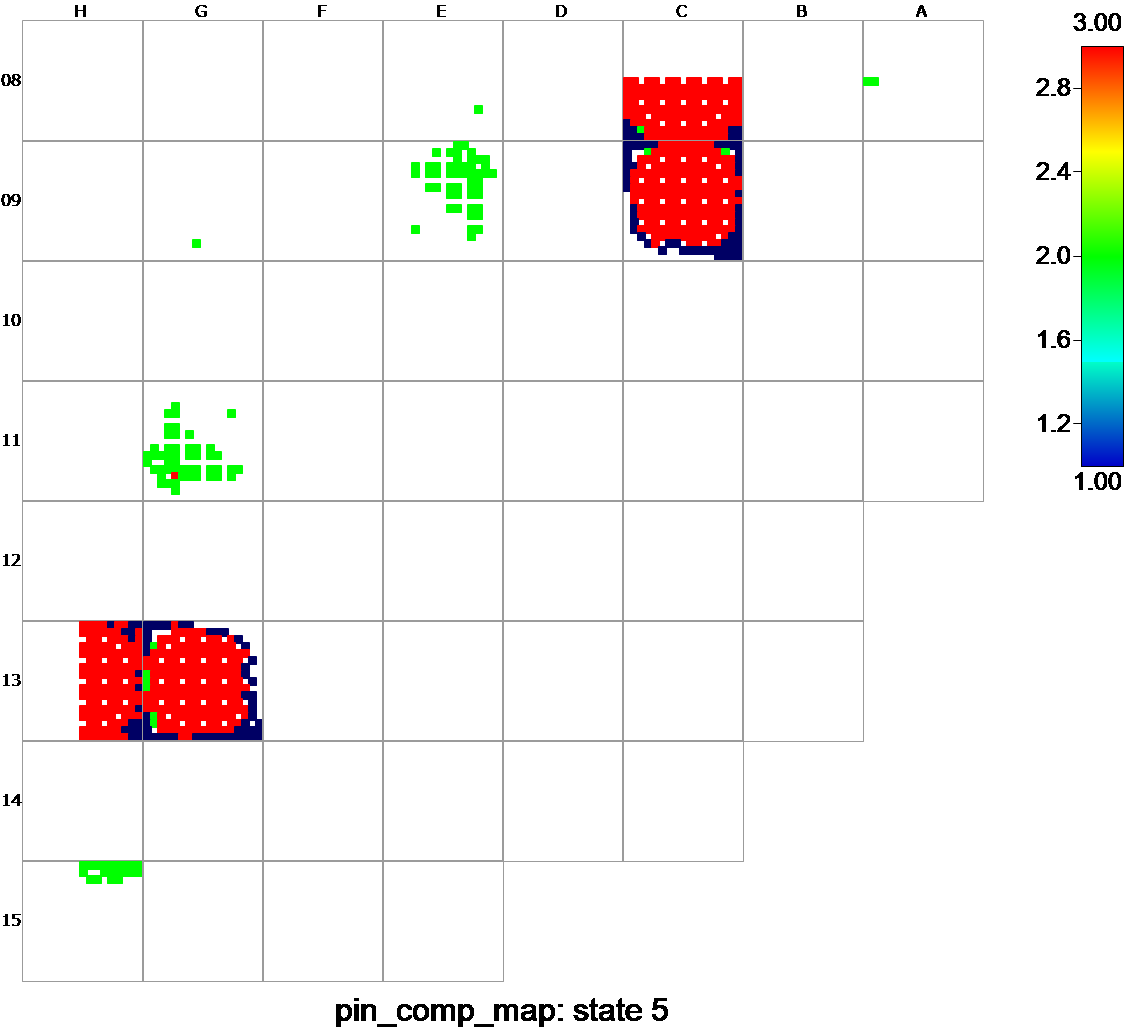
\includegraphics[trim={0 0 4.5cm 0},clip,width=0.4\linewidth]{./Figures/screening/comp5.png}} 
\end{tabular}
\caption{Comparison of the 1000 fuel pins with this highest maximum clad hoop stress and the 1000 fuel pins with the highest weighted change in linear heat rate.}
\label{fig:comp}
\end{figure}
\end{center}
%%%%%%%%%%%%%%%%%%%%%%%%%%%%%%%%%%%%%%%%%%%%%%%%%%%%%%%%%
%%%%%%%%%%%%%%%%%%%%%%%%%%%%%%%%%%%%%%%%%%%%%%%%%%%%%%%%%
\chapter{Conclusions}
%%%%%%%%%%%%%%%%%%%%%%%%%%%%%%%%%%%%%%%%%%%%%%%%%%%%%%%%%
%%%%%%%%%%%%%%%%%%%%%%%%%%%%%%%%%%%%%%%%%%%%%%%%%%%%%%%%%

In order to reduce the computational burden associated with ensuring safe operation of a \gls{PWR} during load-follow operation, a pin based screening process was developed.
The screening process relied on the results of several \gls{VERACS} calculations, where PWR1 was simulated over a period of five cycles.
Excellent agreement was observed between the PWR1 simulations and plant measured data.
Although the predicted response showed an overestimation of the \gls{AO} swing following a power maneuver, the MPACT linear heat rates were able to provide conservative boundary conditions for BISON fuel performance simulations.
A total of 6 power maneuvers, including the start-up power maneuver, were simulated using BISON to determine the limiting fuel pin for each maneuver.

The BISON calculations provided valuable insight on the effect load-follow operation has on fuel rods early in the cycle.
Strong correlations were not observed between the depth of the power change and the stress applied on the cladding upon return to full power.
Power decreases up to 30 \% showed similar maximum cladding hoop stress with power decrease as shallow as 15 \%.
In cases where an intermediate power level was held before returning to full power, the state of the cladding did not vary when compared to a single power escalation.
Similarly, the amount of time low power operation was held did not have an effect on the maximum clad hoop stress for the power maneuvers simulated.
This allows for the conclusion that fuel deconditioning does not occur at the hour time scale.
Additionally, successive power maneuvers did not increase the stress on the cladding in the final return to full power.
This suggests that repeated load-follow operation does not cause increased stress on the fuel rods even when the axial offset is not being tightly maintained.

In order to reduce the computational cost associated with the BISON fuel performance calculations, a weighted linear heat rate was used to screen the core model.
The objective of the screening process was to contain the limiting fuel pin, determined using the clad hoop stress, within the selected 1000 pins.
For all load-follow power maneuvers simulated, the screening process was able to capture the limiting fuel pin.
Additionally, the majority of the fuel pins selected by the screening process showed elevated maximum hoop stresses, although some fuel assemblies were wrongfully identified.
The primary cause of the discrepancy between the screened pin and those that showed elevated maximum hoop stresses was concluded to be the weighting by the linear heat rate.
Early in the cycle, the high linear heat rate of fresh assemblies causes adjacent fuel assemblies to also have elevated linear heat rates, skewing the weighting. 
Later in the cycle, when the power profile of the core is flatter, the linear heat rate will not contribute significantly to the screeningi, process preventing this discrepancy from occurring. 
Nonetheless, the pin-based screening process has proved successful in capturing the limiting pin following a load-follow power maneuver. 
This capability allows for additional maneuvers to be simulated, pushing the power ramps into a more economic operating regime.

\section{Future Work}

In order to further reduce the computational time required to simulate load-follow operation, the following studies can be performed:
\begin{itemize}
\item{The time step used within \gls{VERACS} should be varied to determine if power ramps can be simulated in single steps.}
\item{The detail of the power history provided to BISON should be reduced to determine if the simulation of previous ramps affects future calculations.}
\item{Load-follow calculations should be performed at \gls{EOC}, where the high burunup fuel is likely to experience significant hoop stresses.}
\item{Extreme load-follow operation, i.e. square wave power maneuvers, should be simulated at \gls{EOC}.}
\end{itemize} 

\backmatter
\bibliographystyle{ans}
\bibliography{Masters}


\end{document}
\endinput
